%
%  Vorlage/Template fuer #EBT
%
%  Created by Prof. Dr. Detlef Kreuz on 2010-08-14.
%  Copyright (c) 2010 . All rights reserved.
%
\documentclass[12pt,toc=bib,toc=listof]{scrreprt}
%\usepackage[ngerman]{babel} 
\usepackage{hhline}
\usepackage{csquotes}			%% inline quote
\usepackage[utf8]{inputenc}
\usepackage[T1]{fontenc}
\usepackage{lmodern}
\usepackage{tgpagella}
%%\usepackage[sc]{mathpazo}
\usepackage{setspace}
\usepackage{pdflscape}
\usepackage{afterpage}
\usepackage{multirow}
\usepackage{caption, subcaption}
\usepackage[multiple]{footmisc} % multiple footnotes at a single use
\usepackage{amsmath} % align*

\usepackage{hyperref}
\hypersetup{
	colorlinks=true,
	linkcolor=blue,
	filecolor=magenta,      
	urlcolor=blue,
	citecolor=blue
}
\usepackage[backend=bibtex,
style=numeric,
bibencoding=ascii
%style=alphabetic
%style=reading
]{biblatex}
\addbibresource{bibliography}

%%%%%%%%%%%%%%%%%%%%%%%%%%%%%%%%%%%%% % (fold)
% Vom Studierenden zu aendernde Werte
\newcommand{\ebttopic}{IPv4 vs IPv6 Anycast Catchment: a Root DNS Study}
\newcommand{\ebtstudentname}{Muhammad Arif Wicaksana}
\newcommand{\ebtstudentid}{S1507850}
\newcommand{\faculty}{Faculty of Electrical Engineering, Mathematics and Computer Science (EEMCS)}
\newcommand{\researchgroup}{Design and Analysis of Communication System (DACS)}
\newcommand{\examcommittee}{Prof. dr. ir. Aiko Pras \\ Dr. Ricardo de Oliveira Schmidt \\ Wouter B. de Vries, M.Sc.}
\newcommand{\defensedate}{August 30\textsuperscript{th} 2016}
\urldef{\ebtstudentmail}{\url}{m.a.wicaksana@student.utwente.nl}
%
%%%%%%%%%%%%%%%%%%%%%%%%%%%%%%%%%%%%% % (end)

\usepackage{ifpdf}
\ifpdf
\usepackage[pdftex]{graphicx}
\else
\usepackage{graphicx}
\fi

\usepackage{pdfpages} % include pdf page (\includepdf)
%% additional packages from draft
\usepackage{parskip}
\usepackage{array} 
\usepackage{enumitem}
\usepackage{threeparttable} % table footnote
\usepackage[toc,page]{appendix}
\newcolumntype{C}[1]{>{\centering\let\newline\\\arraybackslash\hspace{0pt}}m{#1}}
\renewlist{tablenotes}{enumerate}{1}
\makeatletter
\setlist[tablenotes]{label=\tnote{\alph*},ref=\alph*,itemsep=\z@,topsep=\z@skip,partopsep=\z@skip,parsep=\z@,itemindent=\z@,labelindent=\tabcolsep,labelsep=.2em,leftmargin=*,align=left,before={\scriptsize}} % threeparttable
\makeatother

%%
\usepackage[headsepline]{scrpage2}
\pagestyle{scrheadings}
\clearscrheadfoot
\ihead{IPv4 vs IPv6 Anycast Catchment: a Root DNS Study}
\ohead{\pagemark}
\renewcommand*{\chapterpagestyle}{scrheadings}
\renewcommand*{\chapterheadstartvskip}{}


%======original=======================================================
\titlehead{\flushright}
\subject{MASTER THESIS}
\title{\ebttopic}
\author{\ebtstudentname}%\footnote{\ebtstudentid, \ebtstudentmail}}
\date{August 30\textsuperscript{th} 2016}
\publishers{Faculty of }
%======original=======================================================

%\pagestyle{headings}

\usepackage{rotating}

\usepackage{pifont}% checkmark font
\newcommand{\cmark}{\ding{51}}%
\newcommand{\xmark}{\ding{55}}%

\begin{document}
\setlength{\parskip}{1em}
\pagenumbering{roman} 
%\selectlanguage{ngerman}

%-----------------------MAKE COVER--------------------------------------
%\maketitle
\includepdf[pages=1]{cover.pdf}
%-----------------------/MAKE COVER--------------------------------------
\newpage\null\thispagestyle{empty}\newpage

% abstract
\begin{abstract}
	\begin{center}
\textbf{Abstract}
	\end{center}
	Anycast has been extensively used by DNS Root Server operators to improve performance, resilience, and reliability. In line with the migration towards IPv6 networks, 9 out of 11 anycasted Root Servers are running on both IPv4 and IPv6 (dual-stack mode) today. Ideally, both protocols should provide similar performances. Problem arises since operators may have different peering policies for IPv4 and IPv6 networks, which leads to different catchment areas for the same service and potentially different quality of service. In this thesis, we analyze the IPv4 and IPv6 catchments of anycasted Root Servers from control-plane perspective between February 2008 to June 2016 using BGP data from RIPE RIS. We study the evolution and  the differences of the catchment areas over the time. We also develop visualization tool to help operator assess their catchment areas. While we specifically study DNS Root Server, our methodology can be applied to other anycast services as well.
	
	%We find that most Root Servers have relatively high convergence level (50\% to 80\%), except for J- and M-Root. Over the time, the level is increasing in general. Some experience sharp increase, some relatively stagnated, and few experiences temporary decrease. The Root Servers also have different visibility levels, which is influenced by the peering policies rather than the number of instances. 
	
\end{abstract}

%% acknowledgements
\addchap*{Acknowledgements} % (fold)
\label{ack}
First and foremost, I would like to express my gratitude to Ricardo de Oliveira Schmidt for giving me the opportunity to work on this subject and providing support, feedback, and suggestions to improve my thesis. I sincerely thank to the other examination committee, Aiko Pras and Wouter de Vries. Additionally, I also would like to thank Jair, Luuk, and Wouter for being really helpful when I was working at the office. In particular for Jair, who greatly helped me preparing my presentation. 

I gratefully acknowledge the MCIT of Indonesia for funding my study, which allows me to make one of my dreams comes true. I am also grateful to all kind people who helped me throughout my master study at University of Twente whom I cannot mention one by one. May God reward you and accept your good deeds.

Last but not least, I would like to thank my family for supporting me, and especially Pamahayu Prawesti for her patience and unconditional love. 



\tableofcontents

%%%%%%%%%%%%%%%%%%%%%%%%%%%%%%%%%%%%% % List of abbreviations
\addchap{List of Abbreviations} % (fold)
\label{sec:abbr}

\begin{description}
  \item[AS:] Autonomous System	
  \item[ASN:] Autonomous System Number
  \item[BGP:] Border Gateway Protocol
  \item[BMP:] BGP Message Protocol
  \item[CDN:] Content Distribution Network 
  \item[DDoS:] Distributed Denial of Service
  \item[DNS:] Domain Name Service
  \item[FQDN:] Fully Qualified Domain Name
  \item[IP:] Internet Protocol  
  \item[IPv6:] Internet Protocol version 6
  \item[MRT:] Multi-threaded Routing Kit  
  \item[RFC:] Request for Comment
  \item[RIPE:] Réseaux IP Européens
  \item[RIS:] Routing Information Service
  \item[TLD:] Top-level Domain
\end{description}

% chapter abkuerzungsverzeichnis (end)

%%%%%%%%%%%%%%%%%%%%%%%%%%%%%%%%%%%%% % List of figures
\listoffigures

%%%%%%%%%%%%%%%%%%%%%%%%%%%%%%%%%%%%% % List of tables
\listoftables

%\onehalfspacing

\newpage
\pagenumbering{arabic}

%%%%%%%%%%%%%%%%%%%%%%%%%%%%%%%%%%%%% % Introduction
\chapter{Introduction}
\label{ch01:intro}

IP anycast \cite{rfc1546} is a technique to share the same IP address among multiple nodes in multiple locations relying on the routing system to map clients to an anycast node (\textit{one-to-any} connection) based on certain parameters, \textit{e.g.}, server proximity, server load, and so on. It started to gain momentum after the DDoS attack targeting all DNS Root Servers on 2002, causing 9 out of 13 Root Servers to be out of service for a moment. The attack caused the link to be congested, leading to unreachable service experienced by user, even though the servers itself remained fully operational. The use of IP anycast enabled Root Servers operators to mitigate such problem. By spreading their instances around the globe, the DDoS attack can be localized to a certain instance, while instances on the other locations remains functional. Another benefit of anycast is to bring the service closer to the users thus reducing service response time, while at the same time keeping the configuration at user side simple. Today, IP anycast is also employed by other distributed services as well, such as CDN, web hosting, and so on.

Despite of its simplicity, IP anycast is difficult to manage. It is because IP anycast completely depends on the routing system--typically BGP--to select the serving anycast node. BGP itself is well-known for its complexity; mainly because it does not route packets solely based on the shortest path, but also takes into account some other considerations in the form of routing policies. Improper BGP configuration could lead to suboptimal routing, causing worse quality of service. For critical service such as DNS, this is a very important issue, since routing configuration also contributes to the latency experienced by users. DNS is a fundamental Internet protocol where many other protocols are relying on it to operate properly (\textit{e.g.}, mail, web). Slow DNS query results in slow response time to them as well. On another side, the deployment strategy of IPv6 to smoothly replace IPv4 allows the IPv4 and IPv6 coexistence in a network. Ideally both protocols should have similar performances. However, this is not always the case. Study from \cite{7145323} that performed measurements against 100 popular dual-stacked websites shows that the performances are sometimes different. Furthermore, performance over IPv6 paths is comparable to those over IPv4 if the AS-level paths are the same. However, it can be much worse if the AS-level paths differ \cite{Dhamdhere:2012:MDI:2398776.2398832}. It shows that having the knowledge over the global Internet for both IPv4 and IPv6 is important to ensure the anycast service is running similarly.

This thesis assesses the differences between IPv4 and IPv6 service coverage (\textit{catchment areas}) from anycast service. DNS Root Servers is used as the case study, primarily because DNS is the pioneering application that heavily uses anycast. Nevertheless, the methodology used in this thesis can be easily applied to other IP-anycast services as well. Here, this thesis is focused on the control plane aspect, \textit{i.e.}, BGP as the routing system used to deliver packets globally. We obtained data from RIPE RIS project \cite{ripe-ncc-ris} that collects BGP routing information from various locations on the globe. The historical BGP data between the first time Root Servers used IPv6 in the beginning of 2008 and June 1\textsuperscript{st} 2016 is studied. The evolution of IPv4 and IPv6 catchment areas of selected Root Servers over the time period is analyzed and then specifically the differences between them are studied. Finally, a visualization tool to help operator assessing their IPv4/IPv6 catchment areas is also developed.

%This report investigates the current practices and monitoring requirements for (anycast) DNS. The recent studies and works in related fields are investigated in order to get understanding of the state-of-the-art of anycast DNS monitoring activities. The goal of this study is to understand current practices of DNS monitoring and requirements for monitoring anycast DNS, and to represent the data towards operators.

\section{Goals}
\label{ch01:goals}

The goal of this thesis is to assess the differences between IPv4 and IPv6 catchment areas of an anycasted services, with DNS Root Servers as the case study. Therefore, the following main research question (RQ) is used:

\textbf{RQ: How different is IPv4 and IPv6 catchment areas of DNS Root Servers?}

In order to address the main RQ, we define four sub RQs as the following: 

\begin{description}
	\setlength{\itemsep}{1pt}
	\setlength{\parskip}{0pt}
	\item [\textbf{RQ.1}] \textit{\textbf{How can we measure the control plane of anycast DNS system?}} There are several methodologies of anycast measurement found in the literature during the last 15 years. Some relevant measurement projects are also present today. Those are discussed to find the most appropriate one for this thesis.
	\item [\textbf{RQ.2}] \textbf{\textit{How do IPv4 and IPv6 catchment areas evolve over the time?}} With the booming of the Internet, IP networks in general are constantly expanding. Infrastructures are continuously being deployed and network interconnections between organizations are being made. This results in the dynamics of Root Server' anycast networks over the time as well. 
	\item [\textbf{RQ.3}] \textbf{\textit{How different is IPv4 and IPv6 catchment areas?}} IPv6 networks are built years after IPv4 ones, and not as vast as its predecessor yet. It is interesting to find out to what extent the difference is from control-plane perspective.
	\item [\textbf{RQ.4}] \textbf{\textit{How to represent the knowledge to the operator?}} Visualization is the best method to represent the knowledge of the networks, so that the operator may  easily assess the IPv4 and IPv6 catchment areas of their anycast service.
\end{description}

\section{Structure}
\label{ch01:structure}
This thesis is organized as follows. Chapter \ref{ch02} provides related background knowledge of this thesis and state-of-the-art of anycast measurement, especially from control-plane perspective. It provides partial answer for RQ.1. Chapter \ref{ch03} explains about our methodology and considerations used in this thesis. It provides the final part for RQ.1 answer. Chapter \ref{ch04} discusses about the result of this work. It provides the answers for RQ.2, RQ.3, and RQ.4. Finally, Chapter \ref{ch05} concludes this thesis by providing the concluding remarks and future works.

%%%%%%%%%%%%%%%%%%%%%%%%%%%%%%%%%%%%% % Background & state-of-the-art
\chapter{Background}
\label{ch02}
This chapter discusses relevant topics to this thesis and state-of-the-art of anycast measurements. It is started with the concept of DNS (Section \ref{ch02:dns}) and IP anycast (Section \ref{ch02:anycast}). Next, methodologies used for anycast DNS measurements as described in the literature are discussed in Section \ref{ch02:measuring-anycast}. Subsequently, the measurement of catchment areas from control-plane perspective is described in Section \ref{ch02:control-plane}. Then, state-of-the-art of anycast visualization is discussed in Section \ref{ch02:visualization}. Section \ref{ch02:concluding} provides the concluding remarks of this chapter.

\section{DNS}
\label{ch02:dns}
As described in RFC 1034 \cite{rfc1034}, \textit{Domain Name System} (DNS) is a distributed database system that essentially provides mapping between IP address and the corresponding name, and vice versa. The data for the mapping is stored in an inverted-tree-structured distributed database (Figure \ref{fig:dns-tree}), where each node is called \textit{domain}. The topmost level of the hierarchy is called the \textit{root domain}, represented by a single dot ('.'), and becomes the starting point of a query. The next level consists of \textit{top-level domains} (TLDs), \textit{e.g.}, \texttt{.com}, \texttt{.net}, \texttt{.id}, and so on. Each domain becomes the root of  a new \textit{subdomain}. Every domain has a unique name, called \textit{fully-qualified domain name} (FQDN), which is the sequence of labels from the node at the root of the domain to the root domain. Each domain can be divided further into \textit{subdomains}, and responsibility for each subdomain can be delegated to a different organization.

\begin{figure}
	\centering
	\includegraphics[scale=0.45]{img/dns-tree.png}
	\caption{Example of DNS database tree}
	\label{fig:dns-tree}
\end{figure}

The DNS has three major components \cite{rfc1034}:
\begin{description}
	\setlength{\itemsep}{1pt}
	\setlength{\parskip}{0pt}
	\item[The domain name space and resource records] A domain name \cite{rfc1035} identifies a node, and the goal of domain names is to provide a mechanism for naming resources (re-corded as \textit{resource records}, RRs) in such a way that the names are usable in different hosts, networks, protocol families, and administrative organizations. 
	\item[Nameservers] Nameservers manage two types of data. Firstly, it maintains \textit{zones}, where each zone is the complete database for a particular segment of domain space (called authoritative). Secondly, it keeps \textit{cached data} acquired by local resolvers, and used to improve the performance of query process when non-local data is frequently accessed. Nameservers also have pointers to other name servers that can be used to lead to information from any part of the domain tree. 
	\item[Resolvers] The local agent that accesses	 nameservers due to query requests from clients. It handles a nameserver queries, response interpretation, and returning the information to the requesting clients. 
\end{description}

\textit{Root nameservers}, shortly called \textit{Root Servers}, is the nameservers for root zone. It contains information of the authoritative nameservers for each of TLD zones. Any DNS queries, except for queries in the authoritative list of a nameserver, requires a response from a root server to be answered (and the answer can be cached for some determined time). 

Root Servers role is critical in DNS because they are needed for the first step of DNS translation. Without them, the DNS simply does not work. Considering that DNS becomes one of the fundamental protocol in Internet infrastructure, failure in DNS may results in major broken connectivities. Currently, there are 13 Root Servers in the world (named from \texttt{A} to \texttt{M}) managed by different organizations, with the names in the form of \texttt{<alphabet>.root-servers.net}. The comprehensive information about Root Servers and their distributions around the world are available in \cite{site:root-servers}.

%The TLDs are categorized into two: \textit{gTLDs} and \textit{ccTLDs}. gTLD is \textit{generic}, in the sense that it can be (theoretically) used by anyone and anywhere. Some well-known examples are \texttt{.com}, \texttt{.net}, and \texttt{.org}. ccTLDs are assigned to countries based on ISO 3166\footnote{\url{http://www.iso.org/iso/country_codes}} list of country codes. Examples are \texttt{.nl}, \texttt{.uk}, \texttt{.it}, and \texttt{.id}.

%To identify resource, RR has the following information: \textit{owner}, which is the domain name where the RR is found; \textit{type}, to specifies the type of the resource; \textit{class}, to identify a protocol family; and \textit{TTL} of the RR. Typically, the most used class is \textit{Internet} (\texttt{IN}). Another one is \texttt{CHAOS} (from Chaosnet protocol \cite{chaosnet}), of which now is used for name server instance identification \cite{rfc4892}. Some examples of RR types are \textit{\texttt{A}}, which is used for host-to-IPv4 address record; \textit{\texttt{AAAA}} for host-to-IPv6; \textit{\texttt{PTR}} for host-to-IP address; and \textit{\texttt{MX}} for mail exchange information. Recently, \textit{\texttt{DS}} and \textit{\texttt{DNSKEY}} have also gained popularity with the increasing deployment of DNSSEC \cite{rfc4641}. The complete list of the classes is available at \cite{iana-dnsparam}. 

%In production environment, it is likely that a single IP address of a DNS server is in fact shared by multiple servers. It might be because of load balancing purpose or the use of anycast. RFC 4892 \cite{rfc4892} provides recommendation on how to identify DNS server. It recommends to query a \texttt{TXT} resource record in class 3 (\texttt{CHAOS}) for the domain name \texttt{HOSTNAME.BIND}. The administrator can then configure this by the unique identifier of the responding server.

\section{IP Anycast}
\label{ch02:anycast}

RFC 1546 \cite{rfc1546} describes IP anycast as a technique to share IP address in common among multiple nodes in multiple locations relying on the BGP routing to map clients to anycast nodes (\textit{one-to-any} connection). Figure \ref{fig:anycast} illustrates conceptual anycast. A client (red node)  sends datagrams towards an anycast address, which is assigned to a group of nodes (green ones). The routing scheme on the network will deliver the datagrams towards \textit{one} of the green nodes which satisfies the best-fit requirement (typically the shortest topological distance). Anycast is intended for services where the users are only care about the service delivery, regardless which server provides it. 

\begin{figure}[ht!]
	\centering
	\includegraphics[scale=0.5]{img/anycast.png}
	\caption{Illustration of anycast (copied from \cite{wiki-anycast})}
	\label{fig:anycast}
\end{figure}

There is also another type of anycast, called \textit{application-layer anycast} \cite{631176}. As the name implies, it works at the application layer. In contrast, IP anycast works in network layer. This thesis focuses on IP anycast only. For the rest of this report, \textit{IP anycast} and \textit{anycast} are used interchangeably.

\iffalse
Despite of its simplicity, IP anycast is known to have some notable limitations \cite{631176,ballani2005towards}: 
\begin{description}
	\setlength{\itemsep}{1pt}
	\setlength{\parskip}{0pt}
	\setlength{\parsep}{0pt}
	\item \textbf{Poor scalability}. Deploying IP anycast globally requires an adequate size of address block (\textit{i.e.}, /24) in order to be properly advertised in BGP by its upstream ISP. On the other hand, routes for IP anycast groups cannot be aggregrated, since the routing infrastructure must support one route per IP anycast group. 	
	\item \textbf{Only suitable for connectionless application}. IP anycast forwarding is performed per-datagram basis. Thus, if there is route changes in the network during transmissions, sequence of packets might be traversed through different paths. This will break applications based on stateful connection. 
	\item \textbf{It only uses shortest path metric to determine the closest server}. IP anycast is unaware of network performance. It also unaware of server load. Thus, it does not provide flexibilities for providers to select their own criteria for choosing the best-fit node, such as the least server load, etc.
	%\end{itemize}
\end{description}

Due to the factors above, the implementation of IP anycast was originally limited and mainly used in low-level protocols, such as  anycasted DNS Root and TLD servers (the main subject of this study), IPv4-to-IPv6 transitioning \cite{rfc3068}, and  AS112 project \cite{rfc7534}. Having more understanding over anycast characteristics and working around the limitations \cite{Ballani:2006:MDP:1177080.1177109,Alzoubi:2011:PAA:2019643.2019644}, more people are starting to look into anycast and apply it to other applications. Studies from Renesys \cite{madory2013anycasters} and Cicalese et al. \cite{cicalese2015characterizing} reveals that big players of the Internet (Google, Microsoft, CloudFlare, OpenDNS, Facebook, and many others) provide a number of services with anycast in their production network, for example: content distribution, web acceleration, cloud services, web hosting, and DDoS protection.
\fi
%\subsection{Anycast in DNS Operations}

The use of anycast in DNS operation was initially motivated by a DDoS attack targeting all DNS root servers on October 21\textsuperscript{st} 2002. The attack \cite{site:21oct}, which congested the Root Server's upstream link, caused 9 out of 13 Root Servers to be unreachable. This resulted, among others, in anycasting the Root Servers. A number of Root Servers' instances configured with the same IP address are spread to different locations across the globe. Therefore, if another attack hits a Root Server's node, the other servers in different locations remain operational, and service disruption can be localized. This approach proved to be effective when on February 6\textsuperscript{th} 2007 another DDoS attack launched against at least 6 Root Servers, and only two of them were noticeably affected because those were not anycasted yet \cite{site:icann-fact}. As the result, up to 72\% TLD servers are anycasted in 2013 \cite{6566965}, and today all Root Server--except B and H--implement anycast \cite{site:root-servers}. 

On the other hand, DNS protocol itself perfectly matches anycast characteristics. Most of DNS communication occurs over either single datagrams or short-lived TCP flows. It fits IP anycast narrative which forwards on per-datagram basis. Implementing anycast in DNS operation is beneficial for the following reasons \cite{colitti2006evaluating,rfc4786}:

\begin{description}
	\setlength{\itemsep}{1pt}
	\setlength{\parskip}{0pt}
	\setlength{\parsep}{0pt}
	\item \textbf{Resilience}. As explained before, by anycasting the servers and spread the servers on multiple locations globally, the attack load are localized, hence the users in that area can be served by other anycast nodes unaffected by the attack. If the server is not responding, the router can be reconfigured to withdraw the prefix announcement from that area.
	\item \textbf{Performance.} Deploying nodes topologically close to clients is expected to decrease query times. In addition, distributing nameservers across the globe will help spreading query traffic from users as well, thus reducing loads per server. This is especially useful for root and TLD nameservers which become the center of DNS operations and experience high load of traffic.
	\item \textbf{Reliability.} Deploying nodes closer to clients in different regions decrease the number of hops that DNS queries must traverse, hence reducing the chance of network failure. 
	\item \textbf{Simplicity}. Anycast allows operators to reduce a list of service addresses for each instance to just a single distributed address. 
\end{description}

As explained before, anycast service uses a single address. In global routing (BGP), this address is represented as an address prefix. Based on how the anycast prefix is announced from the anycasted service to the upstream BGP, anycast node can be categorized into \textit{local} and \textit{global} node. The former one is intended to serve only a limited area, while the latter one is to serve the entire Internet. Local nodes are typically configured using BGP \texttt{NO\_EXPORT} or \texttt{NOPEER} flags, so that the BGP peers receiving the anycast prefix advertisements does not forward further. Global nodes path announcement does not use such flags, and is artificially lengthened using AS-path prepending to affect BGP route selection. RFC 4786 \cite{rfc4786} provides detailed guidelines over anycast service deployment within routing systems. The deployment configuration which contains both local and global nodes is said to be \textit{hierarchical}, while if all nodes are globally visible, then it is said to be \textit{flat}.

The topological region of a network within which packets from users directed at an anycast address are routed to one particular node is called \textit{anycast catchment} \cite{rfc4786}. The catchment area is typically defined by the mapping user-to-node that BGP makes. If there is BGP misconfiguration for local node advertisement such as prefix leaking, the catchment will likely be beyond the intended area and may result in non-optimal node selection.

There are three methods used by Root Server operators to announce anycast prefixes\footnote{The upcoming descriptions contain several concepts in BGP, which are explained in Subsection \ref{ch02:control-plane}}: \textit{(i)} operator may use a single AS as the origin AS of the anycast prefixes from all of their instances that directly connected to its BGP peers. \textit{(ii)} Each global instance announces the prefixes from a unique origin AS, as recommended by RFC 6382 \cite{rfc6382}. \textit{(iii)} All instances announce the prefix from a single origin AS, and there is a unique local AS for each instance intentionally put between the origin AS and the peers that used as the physical identifier of the instance at AS-level.

The first method is intended to preserve ASN needed and to ease management overhead, including to prevent inconsistent origin AS problem\footnote{A problem where single prefix is originated by multiple ASes. Generally, it is used as an indication of prefix hijack, where a prefix is announced by an unauthorized AS to withdraw traffic to it}. Most Root Servers implement this technique. As described in \cite{rfc6382}, The second method aims to better detect changes to routing information associated globally anycasted services and for security reasons.  
%(\textit{e.g.}, implementation of RPKI and ROAs per anycast-node, instead of a single ROA and common origin AS to cover all instantiations of anycasted prefixes within the global routing system). 
The downsides are only organizations with numerous ASNs are able to do it, and that the anycast prefixes will regularly appear in inconsistent origin AS report. A and J-Root use this in practice. The last one  is regarded as the compromise between two former methods. It is intended to preserve the inconsistent-origin ASN reports while at the same time to provide instance identification at network-level. The third method is employed by ISC, the operator of F-Root.

%\section{BGP}
%\label{ch02:bgp}
%Autonomous System (AS) is defined as a region in the Internet which is under a single administrative control, and is identified by a globally unique AS number (ASN), allocated by Regional Internet Registries (RIR). BGP \cite{rfc4271} is the \textit{de-facto} inter-AS routing protocol, which is primarily used to exchange network reachability information (at IP address prefixes level, or simply referred as \textit{prefixes}) with other BGP systems by making routing decisions based on paths, network policies, or pre-configured rule-sets. 

%In initial BGP session, neighboring BGP routers (called as \textit{peers}) exchange their full BGP routing tables. Afterwards, a BGP router may send an announcement of a new route for a prefix or a withdrawal of a route that is no longer available in the form of BGP Update messages. BGP Update message contains information such as routing policy attributes, network-layer reachability information (NLRI) composed of prefix and its length, and path attributes such as list of AS used to reach the prefix originator (\textit{AS path}), next hop IP address, multi exit discriminator (MED), local preference, and so on. This information is used to construct a loop-free graph of AS connectivity for this reachability, from which some AS-level policy decisions may be enforced. For more detailed information regarding BGP messages and path attributes, reader is suggested to refer \cite{rfc4271}.

%\BGP routers typically receive multiple AS paths to the same destination. In order to select the best path, the following priorities based on the attached path attributes are used \cite{1208929}:

%\begin{enumerate}[noitemsep,nolistsep]
%	\item Accept the advertisement with the highest local preference
%	\item Break ties by accepting the advertisement with the
%	shortest AS path
%	\item Break ties by preferring the route with the lowest origin
%	type
%	\item Break ties by accepting the advertisement with the
%	smallest MED for routes with the same next-hop AS
%	\item Break ties by preferring an external BGP advertisement over an internal BGP advertisement
%	\item Break ties by preferring advertisement with the
%	smallest intra-domain cost (IGP metric) to the egress
%	border router
%	\item accepting the advertisement with the smallest next-hop address
%\end{enumerate}

%\subsection{BGP and Anycast}
%In order to be reachable by clients, the prefix of anycasted service should be announced via BGP. \cite{deploying-ip-anycast} provides best practice guidelines to deploy IP anycast on BGP. Current practice is to assign anycast addresses from unicast IP space. In case of Root Server, only a single IPv4 or IPv6 IP addresses is used by the client for simplicity reason. However, BGP practices typically does not allow an AS to originate a single IP address. The typical smallest subnet allowed to be announced is \texttt{/24} for IPv4 and \texttt{/48} for IPv6.

%Based on how the anycast prefix is announced from the anycasted service to the upstream BGP, anycast node can be categorized into \textit{local} and \textit{global} node. The former one is intended to service only a limited area, while the latter one is to service the entire Internet. Local nodes are typically configured using BGP \texttt{NO\_EXPORT} or \texttt{NOPEER} flags, so that the peers receiving the anycast prefix advertisements does not forward further. Global nodes path announcement does not use such flags, and is artificially lengthened using AS-path prepending to affect BGP route selection. RFC 4786 \cite{rfc4786} provides detailed guidelines over anycast service deployment within routing systems. The deployment configuration which contains both local and global nodes is said to be \textit{hierarchical}, while if all nodes are globally visible, then it is said to be \textit{flat}.

%The topological region of a network within which packets from users directed at an anycast address are routed to one particular node is called \textit{anycast catchment} \cite{rfc4786}. The catchment area is typically defined by the mapping user-to-node that BGP makes. If there is BGP misconfiguration for local node advertisement such as prefix leaking, the node will still be treated as local, but the catchment will likely be beyond the initially intended area.

%Some Root Servers implement open peering policy. Some do not mention it, especially the ones operated by commercial organization.


%Global vs regional anycast \cite{anycast-lessons-learned}. Choosing large ISP, they typically prefer cold potato routing, where traffic is prioritized to stay in their network instead of choosing the best exit. Traffic can be moved further than expected. It could result in non-optimal instance selection. Each transit has a different catchment area, and it is different between regions and ASes. Thus, whenever possible, use regional anycast (?).

%While short paths does not necessarily guarantee better user experience, it helps in many ways \cite{Chiu:2015:WOH:2815675.2815719}. It only involves invested parties, optimal use of BGP routing policy mechanism (MEDs and communities) that usually do not propagate past one hop, possibility for joint traffic engineering, prevent spoofed traffic, limiting prefix hijacks, and speeding route convergence.

\section{Anycast Measurement}
\label{ch02:measuring-anycast} 

%Anycast measurement is important because not only it is required to keep an eye on the service, but also because we cannot simply distribute the replicated servers around the world and expecting all users to automatically benefit better service. IP anycast works at network layer, therefore it completely depends on routing system--typically BGP--to select the serving anycast node. The fact that BGP is generally controlled by other people makes anycast service management more complicated. Additionally, some BGP-related problems may affect anycasted services, such as sub-optimal routing selection, route flapping, prefix leaks, and rogue anycast node appearance. Those problems are difficult to diagnose because anycast involves instances at multiple locations.

%There are several anycast measurement methodologies used in the literature, which are summarized in Table \ref{table:ch02:measurement-class}. Latency measurement is performed to get the degree of server proximity from the round-trip time (RTT). To identify node switches, the identity of the serving instance should be known beforehand as well. One common method for node discovery is by sending particular type of DNS query, \texttt{CHAOS TXT} for domain \texttt{HOSTNAME.BIND}. Typically, DNS operators put the information of their instance ID in this form. Traversed path demonstrates the route taken from user to a serving instance. This information may be used to identify node switches and to pinpoint the location of network changes. Service availability information can be acquired by monitoring the presence of query responses from the server. Probes are periodically sending DNS query towards anycast address, and examine the response. No-response means that there is service outage.

\iffalse
\begin{table}[!ht]	
	\begin{center}
		\begin{tabular}{p{6.5cm} p{6.5cm}}
			\hline
			\multicolumn{2}{l}{\textbf{Latency measurement}} \\
			\hline\hline
			ICMP ping & \cite{colitti2006evaluating,cicalese2015first,cicalese2015characterizing,cicalese2015fistful,analysing-k-root,cicalese2015latency} \\
			%			\hline
			query response time & \cite{karrenberg2005anycast,sarat2006use,colitti2006evaluating,Ballani:2006:MDP:1177080.1177109,5488355,aminvisualization}\\
			%			\hline
			traceroute & \cite{yumeasuring,madory2013anycasters} \\
			\hline
			\multicolumn{2}{l}{\textbf{Availability}} \\
			\hline\hline
			Via responses from DNS query & \cite{karrenberg2005anycast,sarat2006use,5488355} \\
			\hline
			\multicolumn{2}{l}{\textbf{Instance discovery}} \\
			\hline\hline
			\texttt{CHAOS TXT} or \texttt{HOSTNAME.BIND} query & \cite{colitti2006evaluating,hiebert2006determining,report:fan2011identifying,yumeasuring,6566965,analysing-k-root,cicalese2015latency,aminvisualization}\\
			\hline
			\multicolumn{2}{l}{\textbf{Instance switches}} \\
			\hline\hline
			Server-side measurement & \cite{barber2004life, colitti2006evaluating} \\
			%			\hline
			Client-side measurement & \cite{karrenberg2005anycast,boothe2005dns,sarat2006use,hiebert2006determining,Ballani:2006:MDP:1177080.1177109} \\
			\hline
			\multicolumn{2}{l}{\textbf{Traversed path}} \\
			\hline\hline
			Traceroute & \cite{report:fan2011identifying,yumeasuring,madory2013anycasters}\\
			%			\hline
			BGP & \cite{boothe2005dns,Ballani:2006:MDP:1177080.1177109,levine2006operational,gibbard2007observations,liu2007two,yumeasuring,madory2013anycasters}\\
			\hline
			\multicolumn{2}{l}{\textbf{Service metrics}} \\
			\hline\hline
			Packet trace & \cite{levine2006operational, liu2007two,6314173,cicalese2015first} \\
			%			\hline
			Server log analysis & \cite{Calder:2015:APA:2815675.2815717} \\
			\hline
		\end{tabular}
	\end{center}
	\caption{Classification of measurement methodologies in the literature}
	\label{table:ch02:measurement-class}	
\end{table}
\fi

Recall that anycast is a distributed service. Thus, it also requires distributed probes as user representations to perform measurements. In general, active measurements are performed mainly by sending \texttt{ping}, \texttt{traceroute}, or DNS queries towards anycast instances in regular basis. Passive measurements are typically conducted by analyzing the incoming packet traces or server logs. It can also be done by analyzing routing system information, such as BGP routing table. 

Table \ref{table:measurement-class} summarizes measurement methodologies for anycast DNS used in literature for the last 15 years. Latency measurement is performed to get the degree of server proximity from the round-trip time (RTT). Service availability is measured via responses from regular DNS queries. Then, since users cannot determine which instance to serve them, instance identification is performed by sending DNS query of \texttt{CHAOS.TXT} for \texttt{HOSTNAME.BIND} \cite{rfc4892}. Regular instance identification can further be used to detect serving instance switches (happens due to service outage or network changes). Instance switch can also be performed at server-side by analyzing presence of users' address in all instance logs. To reveal the traversed paths, classic tool \texttt{traceroute} or AS path from BGP routing table can be used.

\begin{table}[!ht]	
	\begin{center}
		\begin{tabular}{p{6.5cm} p{6.5cm}}
			\hline
			\multicolumn{2}{l}{\textbf{Latency measurement}} \\
			\hline
			ICMP ping & \cite{colitti2006evaluating,cicalese2015first,cicalese2015characterizing,cicalese2015fistful,analysing-k-root,cicalese2015latency} \\
%			\hline
			query response time & \cite{karrenberg2005anycast,sarat2006use,colitti2006evaluating,Ballani:2006:MDP:1177080.1177109,5488355,aminvisualization}\\
%			\hline
			traceroute & \cite{yumeasuring,madory2013anycasters} \\
			\hline
			\multicolumn{2}{l}{\textbf{Availability}} \\
			\hline
			Via responses from DNS query & \cite{karrenberg2005anycast,sarat2006use,5488355} \\
			\hline
			\multicolumn{2}{l}{\textbf{Instance discovery}} \\
			\hline
			\texttt{CHAOS TXT} or \texttt{HOSTNAME.BIND} query & \cite{colitti2006evaluating,hiebert2006determining,report:fan2011identifying,yumeasuring,6566965,analysing-k-root,cicalese2015latency,aminvisualization}\\
			\hline
			\multicolumn{2}{l}{\textbf{Instance switches}} \\
			\hline
			Server-side measurement & \cite{barber2004life, colitti2006evaluating} \\
%			\hline
			Client-side measurement & \cite{karrenberg2005anycast,boothe2005dns,sarat2006use,hiebert2006determining,Ballani:2006:MDP:1177080.1177109} \\
			\hline
			\multicolumn{2}{l}{\textbf{Traversed path}} \\
			\hline
			Traceroute & \cite{report:fan2011identifying,yumeasuring,madory2013anycasters}\\
%			\hline
			BGP & \cite{boothe2005dns,Ballani:2006:MDP:1177080.1177109,levine2006operational,gibbard2007observations,liu2007two,yumeasuring,madory2013anycasters}\\
			\hline
			\multicolumn{2}{l}{\textbf{Service metrics}} \\
			\hline
			Packet trace & \cite{levine2006operational, liu2007two,6314173,cicalese2015first} \\
%s			\hline
			Server log analysis & \cite{Calder:2015:APA:2815675.2815717} \\
			\hline
		\end{tabular}
	\end{center}
	\caption{Classification of measurement methodologies in the literature}
	\label{table:measurement-class}
\end{table}

%Anycast works at the network layer, where the instance selection process completely depends on the routing system--typically BGP--of the network. The fact that BGP is largely controlled by other people makes anycast service management more complicated. Deploying anycast nodes in many sites also does not automatically guarantee the quality of the service globally. As demonstrated by Madory et al. \cite{madory2013anycasters}, it is the path traversed by the packets which really determine the latency--not the number of instances--and this path is largely influenced by BGP routing policy of the providers. Thus, IP anycast may suffers from the following problems related to BGP: sub-optimal routing selection \cite{gibbard2007observations, colitti2006evaluating}, prefix leaks \cite{colitti2006evaluating}, route flapping \cite{liu2007two}, and rogue anycast node appearance \cite{6566965}.

In this thesis, we are in particular interested on the path revelation methodologies. Path revelation allows us to reveal anycast catchment areas. It shows reachability and connectivity of a service. \texttt{Traceroute} provides finer granularity compared to BGP's AS path, since it reveals all routers traversed along the path. \texttt{Traceroute} is simple to use, and it reflects the real path used by the service packets as it works on \textit{data-plane} (part of the network that carries user traffic). However, it only provides a constrained view of the routing system and suffers from ambiguous results such as incomplete paths due to ICMP filtering along the paths. In contrast, BGP only provides a high-level view of connectivities at AS-level, since it works on \textit{control-plane} (part of the network that makes the routing decision). However, it provides more complete view of the routing system; not only the end-to-end AS-level path from users to the anycast service provider, but also route information towards other ASes as well. In the next section, measurements using BGP routing tables and updates is discussed in depth.
 
\section{Measuring IPv4 and IPv6 Catchment Areas from Control-Plane Perspective}
\label{ch02:control-plane}
The 32-bit IPv4 has been used as the device identifier in the network since the beginning of the Internet, and today we are running out of available IPv4 address space \footnote{\url{http://www.potaroo.net/tools/ipv4/}}. IPv6 is intended to provide much larger address space (128-bit) compared to IPv4 (32-bit) with other advantages as well, such as better security, mobility support, and simplification of network configuration. However, even after its standardization 20 years ago, IPv6 adoption is relatively slow. Study from \cite{Czyz:2014:MIA:2619239.2626295} reveals that the number of IPv6 prefixes advertised in BGP has been increasing 37-fold between 2004 and 2014, compared to four-fold of IPv4. Nevertheless, the difference is almost two magnitude. Today, the figures have not changed that much, where the advertised IPv6 prefixes is just 0.0507 of IPv4\footnote{\url{http://bgp.potaroo.net/v6/v6rpt.html}, accessed on August 6\textsuperscript{th} 2016}.

Nikkhah et al. \cite{7182788} categorized three major phases of IPv6 adoption: \textbf{(i)} \textit{stagnation }(1995-2009) due to lack maturity of IPv6 initial version and sufficient  IPv4 addresses available, \textbf{(ii)} \textit{emergence} (2009-2012) due to growing incentive to adopt IPv6 and IPv6 quality improvements, and \textbf{(iii)} \textit{acceleration} (2012-), due to IPv4 addresses exhaustion and sufficient IPv6 adoption at the core Internet to ensure quality of IPv6 connection is equal with IPv4. They also demonstrated that prior to 2011, IPv6 performance gap was largely due to its data-plane (\textit{e.g.}, poor hardware/software performances). Starting from 2011, IPv6 was finally equivalent with IPv4 technology-wise and the gap is primarily due to control-plane performance. Often cases where IPv4 and IPv6 paths are different primarily because of adoption decisions. Instead of following the optimized IPv4 path, IPv6 routing is required to travel around routing domains that have either not deployed IPv6 yet or chose not to establish IPv6 peering sessions with their neighbors. 

The discrepancy between IPv4 and IPv6 paths are crucial since it could affect the service quality. Dhamdhere et al. \cite{Dhamdhere:2012:MDI:2398776.2398832} showed that if the AS-level path was the same in both protocols, performance over IPv6 paths is comparable to that over IPv4. However, it can be much worse than IPv4 if the AS paths differ. This is especially important for anycast DNS, since AS path difference could lead to different physical instances as well. Geographically further anycast node results in longer response time, which could degrade the quality of service. Since many protocols relied on DNS to work properly (\textit{e.g.}, e-mail, web, CDN), the overall service quality could get worse as well. 

Therefore, besides performing typical data-plane measurements to assess the service, monitoring IPv4 and IPv6 catchment areas at control-plane level is also important. Before control-plane-based measurement is discussed, the concept of BGP is briefly explained first. 

%Golkar et al. \cite{7119767} observed that the path lengths do not significantly differ between IPv4 and IPv6. However, IPv6 paths change more frequently than IPv4 paths. Load balancing is more common for IPv6 than for IPv4, most likely due to a simpler or more sparse topology that gives more equal-cost paths for ECMP load balancing.

%Bajpai et al. \cite{7145323} compared IPv4 and IPv6 connectivity of dual-stacked hosts to 100 most popular dual-stacked websites. Their study shows that these websites were hosted in CDN, and these CDN clusters were different for IPv4 and IPv6. There were cases where the CDN caches were present for IPv4, but were largely absent for IPv6 leading to higher connection establishment times.

%In 2012, Kühne \cite{update} measured average AS path lengths as seen by RIS collectors. By ignoring AS prepending, the average number of AS hops of IPv4 and IPv6 is 3.9 and 3.5, respectively. They argued that paths in IPv6 networks were generally shorter than IPv4 because IPv6 was mainly deployed in the core of the Internet, hence the tendency of shorter AS hops. As IPv6 deployment reaches the edges of the Internet, it might stabilize and reach the same density level as in IPv4.

%The flattening Internet topology to bring their networks closer to users and bypassing Tier-1 ISPs on many paths, large content providers are assembling their own wide-area networks \cite{gill2008flattening}. It is further confirmed by \cite{Labovitz:2010:IIT:1851275.1851194} that stated that  the majority of inter-domain traffic by volume now flows directly between large content providers, data center/CDNs and consumer networks. 

Autonomous System (AS) is a region in the Internet which is under a single administrative control, and is identified by a globally unique AS number (ASN) allocated by Regional Internet Registries (RIR). BGP  \cite{rfc4271} itself is the \textit{de-facto} inter-AS routing protocol. It is primarily used to exchange network reachability information at IP address prefixes level (referred as \textit{prefixes}) with other BGP systems by making routing decisions based on paths, network policies, or pre-configured rule-sets. AS that announce the presence of a prefix is referred as \textit{origin AS}. In order to get connected with other ASes, an AS may choose to use \textit{transit} service from larger ISP called \textit{upstream provider}, or it may decide to directly interconnect with other AS (\textit{direct peering}). The policies determine which route to choose and to be propagated to the peers. it is largely defined based on the business relationship of the operators. For example, traffic over customers is preferred than over other providers, since it generates more revenue. On the other hand, traffic via direct peering is favored over transit since it minimizes the cost. These factors, among others, are often lead to sub-optimal BGP routing.

A BGP router maintains network reachability information in the \textit{Routing Information Base} (RIB). RIB consists of three parts (Figure \ref{fig:bgp-update}): \textit{(i)} \texttt{Adj-RIBs-In} (unprocessed routing information learned from inbound Update messages received from other BGP speakers), \textit{(ii)} \texttt{Loc-RIB} (local routing information selected by applying local policies to the routing information contained in \texttt{Adj-RIBs-In}), and \textit{(iii)} \texttt{Adj-RIBs-Out} (stores information to be advertised to peers).

\iffalse
BGP routers typically receive multiple AS paths to the same destination. In order to select the best path, the following priorities based on the attached path attributes are used \cite{1208929}:
\begin{enumerate}[noitemsep,nolistsep]
	\item Accept the advertisement with the highest local preference
	\item Break ties by accepting the advertisement with the
	shortest AS path
	\item Break ties by preferring the route with the lowest origin
	type
	\item Break ties by accepting the advertisement with the
	smallest MED for routes with the same next-hop AS
	\item Break ties by preferring an external BGP advertisement over an internal BGP advertisement
	\item Break ties by preferring advertisement with the
	smallest intra-domain cost (IGP metric) to the egress
	border router
	\item accepting the advertisement with the smallest next-hop address
\end{enumerate}
\fi

\begin{figure}[ht!]
	\centering
	\includegraphics[scale=0.5]{img/bgp-update.png}
	\caption{BGP update process (reproduced from \cite{thousandeyes})}
	\label{fig:bgp-update}
\end{figure}

%Network reachability can be seen from two perspectives: control and data planes. Control plane focuses on building the topology as the router sees based on the routing protocol used. This information is available in router's Routing Information Base (RIB) and/or Label Information Base (LIB). Data plane, or forwarding plane, is the actual paths traversed by data packets from the users. RIB within a BGP speaker consists of three distinct things (Figure \ref{fig:bgp-update}): \texttt{Adj-RIBs-In} (unprocessed routing information learned from inbound Update messages received from other BGP speakers), \texttt{Loc-RIB} (local routing information the BGP speaker selected by applying its local policies to the routing information contained in \texttt{Adj-RIBs-In}), and \texttt{Adj-RIBs-Out} (stores information the local BGP speaker selected for advertisement to its peers)


An anycast service, which is essentially a subset of the Internet itself, is identified at network level through its announced prefixes. The anycast prefixes is part of BGP's network reachability information. To understand and analyze how the anycast catchment works at global Internet, the routing protocol running it--\textit{i.e}., BGP--should be used as the reference. However, BGP is a complex protocol, especially due to the presence of different routing policies implemented by participating organizations. One router may have different BGP route toward a specific destination compared to others, and each router has limited view of the Internet topology. Therefore, gaining knowledge of global Internet only from a single BGP router is definitely not sufficient. 

There are three methods available to get BGP routing information from multiple routers: \textit{(i)} using looking glass, \textit{(ii)} collecting BGP routing information by establishing a BGP peering session with routers using collectors, and \textit{(iii)} using BGP monitoring protocol such as BMP. The summary of these methods including well-known monitoring projects using it is presented in Table \ref{table:ch02:monitoring-methods}.

\textit{Looking glass} is a web-based application managed by operators to provide a view into the BGP routing tables of their BGP routers. It is basically an interface to execute limited range of commands inside the routers. It provides real-time information of the BGP state of a router with no possibility to access historical data. Therefore, looking glass is more appropriate for troubleshooting purposes.

%To perform large-scale BGP monitoring, BGP routing information from wide-range locations around the world needs to be collected. Some operators make BGP routing information from their routers available for monitoring purposes. These participating routers act as the probes for BGP measurement at control-plane level. 


%%%%%%%%%%%%%%%%
% sideways table
%%%%%%%%%%%%%%%%
\begin{sidewaystable}
	\centering
	\scriptsize
	\begin{tabular}{C{2cm} C{1cm} C{2.5cm} C{2cm} C{2.2cm} C{2.5cm} C{2.4cm} C{1cm} C{1cm} C{2cm}}
		\hline
		& \textbf{Start} & \textbf{Managing Organization} & \textbf{Collecting Method} & \textbf{Data Accessibility} & \textbf{Collector Locations} & \textbf{Dump Frequency} & \textbf{Historical} & \textbf{(Near) Real-Time} & \textbf{Note} \\
		\hline\hline
		Looking glass & - & Network providers & accessing router's RIB & web interface & - & - & \xmark & \cmark & real-time BGP state\\ \hline
		RIS \cite{ripe-ncc-ris}& 2001 & RIPE NCC & route collectors & MRT file, REST API & Europe, USA, Brazil, Japan, South Africa & RIB 8 hours, Update 5 min. &\cmark & \xmark & REST API via RIPEStat \\ 
		\hline
		RouteViews \cite{route-views} & 1997 & University of Oregon & route collectors & MRT file, XML stream & USA, UK, Serbia, Kenya, South Africa, Australia, Nepal, Japan, Brazil & RIB 2 hours, Update 15 min. &\cmark & \cmark & live stream is accessed using BGPMon \\ 
		\hline
		BGPMon \cite{bgpmon} & 2008 & Colorado State University & route collectors & XML stream & uses RouteViews collectors & - &\cmark & \cmark & archives accessed in MRT and bgpdump formats \\ 
		\hline 
		PCH \cite{pch} & 2010 & PCH & route collectors & MRT file, routing table overview & 100+ IXPs (details not available) & routing table snapshot daily, Update 1 min. &\cmark & \xmark & VPs are only PCH peers\\ 
		\hline
		Caida OpenBMP \cite{caida-bmp} & June 2016 & Caida \& RouteViews & BMP & Stream & uses RouteViews collectors  & RIB 1 hour, Update 1 min. &\cmark & \cmark & Still in experimental phase \\ 
		\hline
	\end{tabular}
	\caption{BGP monitoring methods}
	\label{table:ch02:monitoring-methods}
\end{sidewaystable}

The second method is by deploying BGP route collectors at various Internet exchange points (IXP) in the world. Route collector, simply referred as \textit{collector}, is a host running a collector processes (such as Quagga\footnote{\url{http://www.nongnu.org/quagga/}}) which emulates a router and establishes BGP peering sessions with one or more participating routers (referred as \textit{peers}). Each peer sends BGP Update messages to the collector each time the \texttt{Adj-RIB-out} changes, which reflecting changes to its \texttt{Loc-RIB}. For each peer, the collector maintains \texttt{adj-RIB-out} table built based on BGP Updates received. The collector periodically dumps the maintained \texttt{Adj-RIB-out} (\textit{RIB dump}) and the BGP Update messages (\textit{Update dump}) received from all of its peers since the last dump. Typically, the dump frequencies are few hours for RIB and few minutes for Updates (see Table \ref{table:ch02:monitoring-methods}). This data dump is then archived in MRT Routing Information Export \cite{rfc6396} format. 

There are two well-known global monitoring projects that use this method in large scale, namely RIPE RIS \cite{ripe-ncc-ris} and RouteViews \cite{route-views}. Both projects have been starting collecting BGP routing information from various locations and peers since the end of 1990s and make the archives available for public access\footnote{\url{http://archive.routeviews.org/}}\footnote{\url{https://www.ripe.net/analyse/internet-measurements/routing-information-service-ris/ris-raw-data}}. In fact, both repositories become the main data sources used by researchers to study various subjects, such as routing policies, Internet topologies, security, and so on. The main issue with them is their file-based distribution system and the delay due to dump interval to make the data available. To analyze a certain prefix, for example, user is required to download the dump file of time interval in interest (can be very large in size) which contains data of other prefixes as well. Performing analysis of wide-range time period would require huge amount of storage and bandwidth to download the data. Fortunately, RIPE NCC as the operator of RIS develop RIPEStat \cite{ripestat}, a web-based interface that provides access to any specific resources contained in RIS archives through its REST API. It allows user to access specific routing resource data (\textit{e.g.}, prefix, ASN) in a fast and convenient way.

Other similar projects also exist. Firstly, PCH \cite{pch} provides their BGP routing data accessible for public as well. However, instead of providing the RIB dump, they only provide snapshot of BGP routing table overview from the output command of '\texttt{show ip bgp}'. Furthermore, judging from its dump size that relatively small compared to RIS or RouteViews, we believe that its route collectors only gather information from PCH peers (not from participating organizations such as RIS or RouteViews). Second project is BGPMon \cite{bgpmon}, a distributed BGP monitoring system that provides real-time data stream in XML format for both BGP updates and RIB snapshot. It uses streamlined collectors that allows it to be more scalable on handling large number of peers. Initially, BGPMon used its own infrastructure to perform measurement. Today, it is used by RouteViews to replace Quagga as the collectors and allows RouteViews to provide live feeds. Unfortunately, BGPMon does not provide historical data access in the same way as its live stream. It stores BGP data in MRT and bgpdump formats hence retains the same issue of file-based distribution.

There are limitations with the use of BGP route information from collectors \cite{6027863,Gregori:2012:IAG:2398776.2398803}:
\begin{enumerate}[noitemsep,nolistsep]
	\item The type of information that can be collected is not always the same. Most updates from collectors' peers are \textit{full-feed} (contains the entire \texttt{Loc-RIB}). However, some updates are \textit{partial-feeds} (only a subset of its \texttt{Loc-RIB}) which may go through a filtering process before being sent to the collectors.
	\item The collector can only see what the connected router advertises. It cannot access what BGP updates a peer receives from its neighbors (peers of a peer). To get all routes, the only way is to examine the BGP \texttt{Adj-RIB-In} for each peer.
	\item some ASes are very large geographically, thus the view in each geographical region might be different for each router in that AS.
	\item The number of collectors available are quite limited, and its placement is geographically and topologically biased. The first bias especially happens in RIS, where most of its collectors reside in Europe. Second bias comes from the fact that the collectors receive data from volunteer networks that mostly are large top-tier ISPs. Therefore, many peer-to-peer connections that may be established among ASes at the Internet edges may not detected. The number of ASes that feeding the collectors are also quite small compared to the total advertised ASes on the Internet. Thus, it results in extremely narrow view of the Internet.
	\item The connections between collectors and routers are not reliable all the time. Data loss might occur anytime.
\end{enumerate}

% more about BGPMon

The third method is an attempt to improve some shortcomings above using \textit{BGP Monitoring Protocol} (BMP) \cite{ietf-bmp}. BMP is used to monitor BGP sessions, and the primary improvement over traditional BGP peering method is the capability to access \texttt{adj-RIB-in} to get complete dump of the routes received by a peer (including routes from peers of a peer). Instead of using collector, the participating peers connects to a management station, sends initial dump of all routes for those peers. As peers advertise or withdraw routes, additional updates are sent to the management station. Thus, user is not required to wait until the data dump available. OpenBMP \cite{openbmp} is an open-source implementation of BMP and supported by the latest Cisco and Juniper's OS. It allows to periodically access the \texttt{adj-RIB-in} of a router or to monitor its BGP peering sessions. 

Despite of its promising improvement, unfortunately there is no large-scale project yet that provide their BMP data publicly as RouteViews or RIS do. An experimental project conducted by Caida and RouteViews \cite{caida-bmp} to use OpenBMP on RouteViews collectors is underway to allow real-time and historical data access, which might be available for public in the near future. Therefore, despite of its imperfectness, RIS and RouteViews still provide the largest usable BGP routing datasets.

%\textbf{Read "Determining the Cause and Frequency of Routing Instability with Anycast". They use BGP data as well.}

\section{Anycast Visualization}
\label{ch02:visualization}
BGP route visualization belongs to the domain of graph drawing, which follows theory rules covered by graph theory. It is a visual representation of the vertices (link between ASes) and edges (ASes). Control-plane Anycast visualization itself can be performed using typical methods for BGP visualization. 

There are several related works on visualizing BGP topology. Since 2000, CAIDA has generated \textit{AS core graphs} (also referred as AS-level Internet graphs) representing a macroscopic snapshot of IPv4 and IPv6 Internet topology samples in order to visualize the shifting topology of the Internet over time, both for IPv4 and IPv6 \cite{caida-vis}. It ranks ASes based on their transit degree; the higher the degree the more centered is the AS placement in the graph. Inspired by CAIDA's work, APNIC developed VizAS \cite{vizas} to provide visualization of the BGP peering relationships within a single economy (e.g., a country). It shows two side-by-side IPv4 and IPv6 charts representing the visible autonomous network in the selected economy.

BGPlay \cite{bgplay} is a Java-based tool which displays animated graphs of the routing activity of a certain prefix within a specified interval to visualize the behavior and instabilities of of Internet routing at the AS level. It is fed using relevant BGP update messages for the specified time interval. BGPlay was used by Karrenberg \cite{karrenberg2005anycast} to visualize path changes between instances and probes in his study. To improve its portability, there is a work to implement BGPlay in pure JavaScript, called BGPlay.js \cite{bgplay.js}, which uses routing data in a specified JSON format. It is currently being used in RIPEstat \cite{ripestat}. 

%AUTOMATTIC, which hosts \texttt{wordpress.com},  provides visualization of their global anycast network at \cite{ac-map}. They develop Netflow-based monitoring system with one of its capabilities is to identify non-optimal anycast networks\footnote{\url{https://developer.wordpress.com/2016/02/08/open-source-netflow-with-elastic-logstash-kibana/}}.

\begin{figure}[!ht]
	\begin{subfigure}[b]{0.5\linewidth}
		\centering
		\includegraphics[width=\linewidth]{img/beforeAmestC.png}
		\caption{Control plane - before}
		\label{fig:ricardo-control-before}
	\end{subfigure}
	\begin{subfigure}[b]{0.5\linewidth}
		\centering
		\includegraphics[width=\linewidth]{img/afterAmestC.png}
		\caption{Control plane - after}
		\label{fig:ricardo-control-after}
	\end{subfigure}
	\caption{Visualization of routing impact of adding or removing anycast instances, copied from \cite{github-anycast}}
	\label{fig:ch02:ricardo}		
\end{figure}

Specific to anycast visualization, the authors of \cite{github-anycast} proposed visualization tool for IP anycast to understand routing impact of adding or removing instances. Since BGP paths consist of a number of AS hops, it would be easier to understand if ASes with the same hop degree relative to the measured AS are grouped together. Thus, they use radial tree graph based on the Reingold-Tilford algorithm \cite{1702828} for efficient, tidy arrangement of layered nodes. They use PEERING platform \cite{peering} as the anycast testbed consisting of 7 instances spread in USA, Brazil, and the Netherlands. They use a subset of RIPE Atlas probes that periodically run \texttt{traceroute} towards PEERING. The BGP routing data is collected from both \texttt{traceroute} and RIS collectors. The tool separates the view into two segments: control and data planes. Control plane visualization is used to see the changes in BGP routes when there is a change (withdrawal or announcement) of an instance. The data is taken from RIPE RRC. In order to quantify changes take place in data plane, a periodic traceroute measurements are performed using RIPE Atlas probes. The result of their visualization for control plane is presented in Figure \ref{fig:ch02:ricardo}. It shows the anycast catchment areas before and after the instance announcement. The ASes are arranged in a hierarchy based on the degree towards the origin AS.  

To summarize, CAIDA's graph and VizAS are impressive. They are intended to visualize high-level overview of the topology by focusing more on who are the big players in the networks. Since the diameter of the outer circle is fixed, as the networks become larger with huge numbers of edge ASes then the graph becomes difficult to read due to denser outer circle. BGPlay excels at visualizing AS-level network changes over a period of time. As it visualizes every BGP Update message events, it provides very detailed information. Thus, BGPlay is more suitable as troubleshooting tool. Result from \cite{github-anycast} is the closest to the requirement of this work. Improvements can be made, especially in the interactivity part.

\section{Concluding Remarks}
\label{ch02:concluding}
%\texttt{Traceroute} and BGP routing information are the two methods used in the literature in Section \ref{ch02:measuring-anycast} to reveal anycast catchment areas. Despite of its simplicity and finer granularity, \texttt{traceroute} suffers from ICMP filtering often implemented along the path. On the other hand, BGP routing data provides high-level view of connectivity, but reveals end-to-end AS-level paths. For this study, using BGP routing data is more appropriate as we need broad view of the networks to understand the catchment areas. There are several methods to obtain BGP routing data, as listed in Table \ref{table:ch02:monitoring-methods}. As we need to study the catchment areas from the beginning of Root Servers' dual-stacked operation, the historical data access is required. The use of BMP is quite promising, due to more complete results offered. However, the large-scale project we know is running it is still in experimental phase and just started recently. Thus, it leaves us with the route collector-based projects as the data repository.
\texttt{Traceroute} and BGP routing information are the two methods used by literature to reveal anycast catchment areas. Despite of its simplicity and finer granularity, \texttt{traceroute} suffers from ICMP filtering often implemented along the path. On the other hand, BGP routing data provides high-level view of connectivity, but reveals end-to-end AS-level paths. For this study, using BGP routing data is more appropriate as we need broad view of the networks to understand the catchment areas. In order to obtain historical BGP routing data, using public data from measurement projects such as RIS and RouteViews is preferred over other approaches. Finally, to visualize comparison of IPv4 and IPv6  anycast catchment area, work in \cite{github-anycast} is the closest to this work, and thus it can be developed further to fit our requirements and to include interactivity features.


%%%%%%%%%%%%%%%%%%%%%%%%%%%%%%%%%%%%% % Methodologies
\chapter{Methodology}
\label{ch03}
This chapter discusses methodology used in this study. Firstly, the selection of Root Servers used is presented in Section \ref{ch03:root-server}. Secondly, the method used to retrieve historical BGP data is discussed in Section \ref{ch03:bgp-data}. Thirdly, types of data analysis performed and considerations taken is presented in Section \ref{ch03:analysis}.  Fourthly, visualization technique we used in Section \ref{ch03:visualization}. Finally, the concluding remarks of this chapter is provided in Section \ref{ch03:concluding}.

\section{Selecting Eligible Root Servers}
\label{ch03:root-server}
As discussed in Section \ref{ch02:dns}, there are 13 Root Servers in operation today. However, not all of them are eligible for this study. The objective of this thesis is to assess IPv4/IPv6 catchment areas of anycast service. Thus, we only select Root Servers that are anycasted and provide dual-stacked services. Among all Root Servers, we omit B and H-Root as these Roots are not anycasted yet. We also rule out E and G-Root as those are IPv4 only. Thus, it leaves us with A, C, D, F, I, J, K, L, and M-Root.

\begin{table}[h]
	\centering
	\begin{threeparttable}	
		\begin{tabular}{c c c}
			\hline
			\textbf{Root Server} & \textbf{IP Addresses}	& \textbf{IPv6 Starting Date\tnote{a}} \\ \hline\hline
			\multirow{2}{*}{A}	& 198.41.0.4	& \multirow{2}{*}{Feb 2008}  \\ & 2001:503:ba3e::2:30 \\  \hline
			
			\multirow{2}{*}{C}	& 192.33.4.12	& \multirow{2}{*}{Mar 2014}  \\ & 2001:500:2::c \\  \hline
			
			\multirow{2}{*}{D}	& 128.8.10.90, 199.7.91.13\tnote{b}	& \multirow{2}{*}{Mar 2014}  \\ & 2001:500:2d::d \\  \hline		
			
			\multirow{2}{*}{F}	& 192.5.5.241	& \multirow{2}{*}{Feb 2008}  \\ & 2001:500:2f::f \\  \hline				
			
			\multirow{2}{*}{I}	& 192.36.148.17	& \multirow{2}{*}{Jun 2010}  \\ & 2001:7fe::53 \\  \hline						
			
			\multirow{2}{*}{J}	& 192.58.128.30	& \multirow{2}{*}{Feb 2008}  \\ & 2001:503:c27::2:30 \\  \hline								
			
			\multirow{2}{*}{K}	& 193.0.14.129	& \multirow{2}{*}{Feb 2008}  \\ & 2001:7fd::1 \\  \hline	
			
			\multirow{2}{*}{L}	& 198.32.64.12, 199.7.83.42\tnote{c}	& \multirow{2}{*}{N/A}  \\ & 2001:500:3::42, 2001:500:9f::42\tnote{d} \\  
			\hline
			
			\multirow{2}{*}{M}	& 202.12.27.33	& \multirow{2}{*}{Feb 2008}  \\ & 2001:dc3::35 \\  \hline	
		\end{tabular}
		\begin{tablenotes}
			\item \url{http://www.root-servers.org/news.html}
			\item Switched to the second IP address in January 2013
			\item Switched to the second IP address in March 2016
			\item Switched to the second IP address in November 2011
		\end{tablenotes}
		\caption{Root Servers used in this thesis}
		\label{table:ch03:root-servers}
		
	\end{threeparttable}
\end{table}

Table \ref{table:ch03:root-servers} presents all Root Servers used in this study. The selected Root Servers have different starting date of dual-stack operation. Since the majority of them (A, F, H, J, K, M) started using IPv6 from February 2008\footnote{\url{http://www.iana.org/reports/2008/root-aaaa-announcement.html}}, the data analysis is started from March 1\textsuperscript{st} 2008 and ended on June 1\textsuperscript{st} 2016. The other Root Servers (C, D, I) started using IPv6 later. We cannot find information regarding L-Root's starting date. However, based on the BGP routing data, it seems L-Root started to run dual-stacked service at least in February 2008.

Root Servers use single address for each IPv4 and IPv6 for their DNS service. However, some of them changed their addresses during the observation time (second column of Table \ref{table:ch03:root-servers}). These changes are taken into account as well in our analysis program. 

\section{BGP Data Retrieval}
\label{ch03:bgp-data}
As discussed in Section \ref{ch02:measuring-anycast}, there are two projects that provide large-scale historical BGP routing data, namely RIS and RouteViews. Looking at their collector list, RouteViews\footnote{\url{http://archive.routeviews.org/}} has advantage over RIS (Table \ref{table:ch03:ris-collectors}) in terms of collectors distribution. RIS is Europe-centric, where only 6 out of 18 collectors are outside the continent and 3 of them are in USA. On the other hand, RouteViews is more globally distributed. Beyond the US and European countries, RouteViews also deploy collectors in Australia, Singapore, Nepal, and Kenya. Using both data source would be complementary. However, RouteViews only provides the raw MRT files. Typically, each collector produce \textasciitilde100 MB of BGP RIB data for each dump interval that its size keeps growing over the time. Suppose there are 17 collectors. Thus, for the time period used in this thesis (each month between March 2008 and June 2016), we should download $17 \times 100$ MB $\times  88$ months $= 149.6$ GB, not including time required to process the raw data. Due to time and resource constraints in this work, using data from RouteViews is considered to be not feasible. 

On the other hand, RIS collectors data can be accessed through RIPEStat using its API, which allows us to only access specific BGP routing information that we need. Thus, we use RIPEStat as our data provider. We specifically need to access reachability of all RIS collectors' peers in the form of AS paths to a certain prefixes, \textit{i.e.}, the Root Servers' prefixes, at a point of time. To do this, we employ data call \texttt{"BGP State"}\footnote{\url{https://stat.ripe.net/docs/data_api\#BGPState}}. We use the IP address of a Root Server as the argument, instead of its prefix. This is because some operators prefer to announce different anycast prefix lengths to distinguish global and local catchments. For instance, F-Root uses /23 prefix for its global nodes and /24 for local instances, so that routers which possess both routing information will prefer the local instances (if present) as its prefix is more specific. By using Root Server's IP addresses, we hand over the decision of which prefix chosen by the RIS peers for those addresses to the system. For example, to query BGP routing data for IPv4 prefix of M-Root on June 1\textsuperscript{st} 2016, then the following URL is used. Here the date is converted into UNIX timestamp:

\url{https://stat.ripe.net/data/bgp-state/data.json?resource=202.12.27.33&timestamp=1464739200}


\begin{table}
	\centering
	\begin{tabular}{c c c}
		\hline
		\textbf{Code} & \textbf{Location}	& \textbf{Operating Date} \\ \hline\hline
		rrc00	& RIPE NCC, Amsterdam	& Oct 1999 \\ \hline
		rrc01	& LINX, London			& Jul	 2000 \\ \hline
		rrc03	& AMS-IX and NL-IX, Amsterdam	& Jan 2001 \\ \hline
		rrc04	& CIXP, Geneva		& Apr 2001 \\ \hline
		rrc05	& VIX, Vienna		& Jun 2001 \\ \hline
		rrc06	& Otemachi, Japan	& Aug 2001 \\ \hline
		rrc07	& Stockholm, Sweden	& Apr 2002 \\ \hline
		rrc10	& Milan, Italy		& Nov 2003 \\ \hline
		rrc11	& New York (NY), USA	& Feb 2004 \\ \hline
		rrc12	& Frankfurt, Germany	& Jul 2004 \\ \hline
		rrc13	& Moscow, Russia	& Apr 2005 \\ \hline
		rrc14	& Palo Alto, USA	& Dec 2004 \\ \hline
		rrc15	& Sao Paulo, Brazil	& Dec 2005 \\ \hline
		rrc16	& Miami, USA	& Feb 2008 \\ \hline
		rrc18	& CATNIX, Barcelona	& Nov 2015 \\ \hline
		rrc19	& NAP Africa JB, Johannesburg	& Nov 2015 \\ \hline
		rrc20	& SwissIX, Zurich	& Nov 2015 \\ \hline
		rrc21	& France-IX, Paris	& Nov 2015 \\ \hline
	\end{tabular}
	\caption{List of RIS collectors used in this study}
	\label{table:ch03:ris-collectors}
\end{table}

RIPE RIS collectors gather BGP information from participating routers. These peers act as \textit{vantage points} or VPs for our measurement, and from now on we refer them simply as \textit{VPs}. VPs may have IPv4 and/or IPv6 route information towards certain Root Server. Those that possess routes to both IPv4/IPv6 prefixes of a Root Server at a given time are referred as \textit{dual-stacked VPs}. Dual-stacked VPs becomes the primary subject of this thesis since they allow us to perform comparable analysis of IPv4 and IPv6 catchments. 

\begin{figure}
	\centering
	\includegraphics[width=.6\linewidth]{img/configuration}
	\caption{Workflow of this study}
	\label{fig:ch03:config}
\end{figure}

It should be noted from Table \ref{table:ch03:ris-collectors} that the starting operation date among RIS collectors are different. This affects in the total number of the participating peers at a time. However, since the observation period is started in March 2008, the impact of new collectors addition only takes place starting in November 2015. This is particularly reflected in the notable increase of dual-stacked VPs of all Root Servers starting in the end of 2015, as can be seen later in the Chapter \ref{ch04}.

Figure \ref{fig:ch03:config} illustrates the workflow of this study. All BGP data related to Root Servers' prefixes between March 1\textsuperscript{st} 2008 and June 1\textsuperscript{st} 2016 for every first date of each month is retrieved from RIPEStat, and then persisted in two databases. Data from dual-stacked VPs that is used for data analysis is stored in MongoDB. MongoDB is selected because it is document-oriented and the data itself is in JSON format, hence makes the analysis process straightforward. Data from all VPs are stored in the second database, Neo4j, for visualization purpose. Neo4j is a graph database, hence it fits  well with the nature of BGP. It makes the queries for visualization easier. All code and data used throughout this work, including the more detailed technical description, are available at our Github repository \cite{github-thesis}.

To make the visualization informative, short description of ASes is needed. Data provided by Team Cymru Research\footnote{\url{http://www.team-cymru.org/index.html}} is used, which is accessible through their WHOIS service. Initially, we chose to perform real-time WHOIS query to provide visualization interactivity. However, sometimes Cymru does not provide quick response, which leads to poor user experience. Therefore, we decided to download AS information for all unique ASes in the database, so that the visualization front-end can quickly retrieve the data from local database. We believe that this is justified because ASN does not change much, so it is safe to have a copy in local repository.

\section{Data Analysis}
\label{ch03:analysis}

%An anycast instance is typically consisted of multiple servers for redundancy and reliability reasons. This work focuses on control-plane, thus the scope is only up to instance-level. Therefore, there is no need to identify up to server-level.


\begin{figure}
	\centering
	\includegraphics[width=.5\linewidth]{img/as-path}
	\caption{Illustration of AS path definition}
	\label{fig:ch03:as_path}
\end{figure}

The Internet can be modeled as graph, $G=(V,E)$. A vertex in $V$ represents AS, and edges in $E$ are peerings between ASes. An AS path between a source AS (\textit{i.e.}, VP of RIS) $A$ and destination AS $B$ (\textit{i.e.}, the origin AS of Root Server's prefixes)  is defined as $P_{AB}=v_0\rightarrow v_1\rightarrow v_2 \rightarrow ... \rightarrow v_{n}$ where $v_0=AS_A$, $v_{n}=AS_B$, and $n$ denotes the hop number. In this thesis, we say that $P_1$ is identical to $P_2$ if $n_1 = n_2, v_{i1}=v_{i2}$ for $i\in [0,n]$. Otherwise, $P_1$ and $P_2$ are said to have different path. In the case of $n_1 \neq n_2$, we say that $P_1$ is shorter than $P_2$ if $n_1 < n_2$.

% $\exists!v	\in(v_0, v_1, v_2, .., v_{n})$

Figure \ref{fig:ch03:as_path} illustrates AS paths relationship definition above. All paths $P_1$ to $P_5$ have origin AS $A$ and source AS $D$. $P_1$ is identical to $P_2$ since all of their transit ASes are identical. $P_1$ and $P_3$ are said to have different path even though the path lengths are similar, since there is a transit AS for a certain degree that does not identical for both of them. $P_4$ is said to have shorter path than $P_1$, and in contrary $P_5$ has longer path than $P_1$.

Networking communities use the term \textit{peering} to refer BGP session between two networks to exchange traffic between each others, typically for free. The relationship is equal for both sides. Thus, they try to keep the traffic flowing in both directions to be balanced, so that they have bargaining position to keep the connection free. Otherwise, the other party will start to charge them if their traffic is higher than their counterpart. On the other hand, the term \textit{transit} is used to describe paid BGP session between customer and provider where the provider carry all of their customer's traffic (inbound and outbound) to/from the Internet. Since it is difficult to infer the economic relationship between Root Server and their next-hop ASes based on the dataset we have, this thesis uses the term \textit{peering} broadly as its basic meaning, which is the BGP session between two BGP speakers regardless the economic cost, to refer connection between Root Servers' origin ASes with their adjacent ASes.

In this thesis, we perform comparison on IPv4 and IPv6 AS paths of a VP. If a dual-stacked VP has identical IPv4 and IPv6 paths for certain Root Server's prefixes, we refer it as \textit{converging VP}. If the paths are different, then we refer it as \textit{diverging VP}. The amount of dual-stacked VPs and converging VPs of a Root Server at a given of time is an important metric used to determine the convergence level, as discussed later (Section \ref{ch03:analysis:diff}).

To analyze the catchment areas, we address two subjects: \textit{(i)} evolution of catchment areas (Section \ref{ch03:analysis:evolution}),  and \textit{(ii)} the difference between IPv4 and IPv6 catchment areas (Section \ref{ch03:analysis:diff}). 

\subsection{Evolution of Catchment Areas}
\label{ch03:analysis:evolution}
This subject is intended to understand the AS-level dynamics due to changes made by the operators on their networks over the time. In the context of this thesis, we focus to see the dynamics in two things: \textit{(a)} the IPv4 and IPv6 networks becomes either divergent/convergent or intact, \textit{(b)} the average path lengths over the time. Thus, we use all data from VPs that possess route information towards both IPv4 and IPv6 prefixes of the Root Servers (dual-stacked VPs). 

Ideally, IPv4 and IPv6 catchment areas of a certain anycast service should be identical. In another word, IPv4 and IPv6 AS paths towards the anycast service from any given point in the Internet topology should follow the same AS hops. In this way,  IPv4 and IPv6 users experience the same path from control-plane perspective. However, this does not always the case. There are factors leading to different IPv4 and IPv6 paths towards the same destination as experienced by VPs. Firstly, the deployment of IPv6 is not as mature as IPv4 network yet. There are still some parts in the Internet that only provide IPv4 routing capabilities, especially on the Internet edges. Secondly, the network operators may have different policies or peering agreements between IPv4 and IPv6 traffic with other operators. However, Dhamdhere et al. \cite{Dhamdhere:2012:MDI:2398776.2398832} suggests that the deployment of global IPv6 network are \textit{converging} towards global IPv4 network. This can be easily understood since IPv4 network has been around for longer time and has been experiencing many optimizations and fixes of network misconfiguration, and can be considered as mature today. Thus, developing IPv6 networks based on IPv4 infrastructures will benefit from all lessons learned in the past.


To identify the convergence level of a certain anycast service (or service in general), we make use of AS path data from dual-stacked VPs. The fraction of converging VPs of all dual-stacked VPs at a time that see a Root Server's IPv4 and IPv6 prefixes is defined as the convergence level:

\begin{align*}
convergence\: level=\frac{\sum VP_{converging}}{\sum VP_{dual \: stacked}} \times 100\%
\end{align*}

%should make stronger statement for "the idea is to have shorter AS..." by re-read paper 1-hop%
Another aspect from a catchment areas evolution we are interested at is to look at the trends of average path length over the time. The idea is to have shorter AS as possible between Root Server's origin AS and the users. While short paths does not automatically guarantee better user experience (it has to be verified at data-plane level), it generally shows that the distance between two parties are likely to be close. In case of shortest path possible (direct peering), it helps in many ways \cite{Chiu:2015:WOH:2815675.2815719}:  \textit{(i)} it sidesteps potential obstacles in the form of additional transit ASes, \textit{(ii)} it allows optimal use of BGP routing policy mechanism that usually do not propagate past one hop (MED, communities), \textit{(iii)} possibility for joint traffic engineering, \textit{(iv)} prevents spoofed traffic, \textit{(v)} limits prefix hijacks, and \textit{(vi)} speeds route convergence. To understand this in the context of DNS Root service, we calculate the distribution of dual-stacked VP path lengths over the observation period to see the trends.

\subsection{The Differences Between IPv4 and IPv6 Catchment Areas}
\label{ch03:analysis:diff}
On the latter part, we focus on the differences itself as seen by the VPs. Thus, here we only use data from VPs that have different IPv4 and IPv6 paths toward a Root Server origin AS (diverging VPs). The diverging paths could happen because there are different routing policies applied for IPv4 and IPv6. For example, an operator may prefer to transit via provider \textit{A} for IPv4 connectivities to the Internet and provider \textit{B} for IPv6, perhaps due to some advantages offered by \textit{B}. One particular case is Hurricane Electric, which offer free IPv6 peering\footnote{although the traffic allowed to pass through is only for traffic with destination to Hurricane's network or its paid customers}. In fact, diverging route is a common practice we found from the datasets. This convention may results in different IPv4 and IPv6 AS path lengths experienced by the diverging VPs.

There are three aspects discussed here. \textit{Firstly}, the characterization of diverging VPs composition: how many of them experience shorter IPv4, shorter IPv6, and different paths but equal length. This information provides us illustration of an anycasted service's reachability level in IPv4 and IPv6. For example, does it really take care of its IPv6 users as its IPv4 ones? 
\textit{Secondly}, the average path lengths is again studied. Only this time for diverging VPs. Hypothetically, longer AS paths have higher probability to have diverging paths, as it will traverse more intermediate ASes with potentially diverse routing policies, compared to the short one. Longer path also means that the source AS is more likely to be located at the edge of the Internet. As we know, the IPv6 deployment in Internet edges are still lagging. Thus, IPv6 route may take sidestep to round IPv4 only networks, resulting in longer path. \textit{Thirdly}, we would like to know how different it is in terms of AS path lengths for diverging VPs. 

\section{Visualization}
\label{ch03:visualization}

A tool is developed to visualize BGP path data obtained from RIPEStat. It is web-based, so that it can be easily accessed everywhere and integrated with existing monitoring tools. D3.js \cite{d3js}, a JavaScript library for manipulating documents based on data, is used at the front-end to render the graph due to its powerful and rich visualization types. To feed the visualization data, a back-end application based on Flask is developed, which accesses the databases described in Section \ref{ch03:bgp-data}.
%In CAIDA's AS core visualization, the center of the graph are ASes with high transit degree. In contrast to this, our graph resembles a tree, with the root of the tree is the Root Server's AS(es).

The tool is developed based on work result from \cite{github-anycast} (Section \ref{ch02:visualization}). One fundamental difference is the use of forced layout instead of radial Reingold-Tilford tree as used by the authors. While the latter one is excellent on arranging ASes based on their AS path level relative to the origin AS, it constructs the visualization based on each individual VP's AS path. Thus, the transit ASes might be visually duplicated in other part of the graph and does not provide complete picture of the catchment. Forced layout eliminates this by removing hierarchical display and provides visualization as a whole AS interconnections. To compensate the lack of AS path level information, we use color code to group ASes with the same AS path level. To simplify the visualization, AS prepending property is encoded as the thickness of the line connecting two ASes, instead of repeatedly displaying the same AS as sequence of nodes.

Further improvement is made by providing interactivity. Graph can be selected for any particular point of time in the observation period. To allow operator performing comparison, IPv4 and IPv6 catchment areas are displayed side by side with the list of mutual dual-stacked VPs presented below. As the network can grow quite large and complex, the graph elements can be zoomed in and out, panned, and moved for better readability. To make the IPv4/IPv6 path comparison of a certain dual-stacked VPs easier, both IPv4 and IPv6 AS paths are highlighted when it is hovered. The short AS description retrieved from Team Cymru is also displayed on top of it.

\section{Concluding Remarks}
\label{ch03:concluding}
Not all Root Servers can be used in this study because non-anycasted and IPv4-only are excluded. For the data provider, using both RIS and RouteViews would be complementary because they cover different collector placements. However, due to constraints in this work, only RIS is used since it provides easy access to their historical BGP data. Then, some definitions used in the upcoming analysis is described in Section \ref{ch03:analysis}. The subjects of analysis are also presented, covering evolution of catchment areas and the differences between IPv4 and IPv6 catchments itself. Finally, for the visualization, we extend the work from \cite{github-anycast} with a change graph type and improvements in visualization interactivity.

%%%%%%%%%%%%%%%%%%%%%%%%%%%%%%%%%%%%% % Result analysis
\chapter{Result Analysis}
\label{ch04}
The analysis of the work results is provided in this chapter. As described in Section \ref{ch03:analysis}, the analysis is divided into two topics: \textit{(i)} evolution of catchment areas (Section \ref{ch04:evolution}), and \textit{(ii)} the differences between IPv4 and IPv6 catchment areas (Section \ref{ch04:differences}). The features of visualization tool intended to help operator assessing their catchment areas is discussed in Section \ref{ch04:visualizing}. Finally, this chapter is concluded by a discussion about the importance of performing IPv4/IPv6 catchment areas for the operator in Section \ref{ch04:discussion}.

\section{Evolution of Catchment Areas}
\label{ch04:evolution}
Over the time, anycast operators may made changes on their network in order to improve the service. They may have added instances at underserved locations, changed their service policy, made new peering agreements with other organizations, and so on. These changes may result in congruity of the IPv4 and IPv6 catchments, or even higher differences between them. The changes may also not fundamental enough to change the catchment topology, hence it remains relatively the same throughout time. In this subsection, we discuss about the evolution of Root Server's catchment areas from control-plane perspective during the period March 1\textsuperscript{st} 2008 to June 1\textsuperscript{st} 2016.

\subsection{Convergence}
\label{ch04:evolution:convergence}
Recalling from Section \ref{ch03:analysis:evolution}, convergence level is a metric to describe the fraction of converging VPs of all dual-stacked VPs that see certain Root Server prefixes. Convergence levels of all Root Servers are presented in Appendix \ref{app:convergence}, with some are presented in Figure \ref{fig:ch04:convergence}. The blue line represents the convergence level, and the red line indicates the total number of dual-stacked VPs. The inclusion of the dual-stacked VPs into the graphs serves two purposes: \textit{(i)} it can be used as the control when there is outlier data for convergence level. For example, K-Root (Figure \ref{fig:convergence-k}) have convergence level 100\% until the middle of 2009. By observing the number of VPs at the same time period, it is because there was only small number of VPs detected K-Root prefixes hence the skewed result. \textit{(ii)} it can also be used to infer the visibility level of Root Servers as seen by RIS peers, as explained later in this subsection. 

The results show that convergence level of the majority of the Root Servers is relatively high, between 50\% to 80\%, with the exception J- and M-Root that are below 40\%. Most Root Servers’ convergence are varying over the time, which implies that network changes took place during the period. In general, they have tendency to increase over the time. Some experience sharp increase at one point in time (A, D), some are steadily increasing (K, L), and some are relatively stagnated (I, C). Only D and M-Root that experience a notable temporary decreasing moment.

\begin{figure}[h]
	\begin{subfigure}{.5\textwidth}
		\centering
		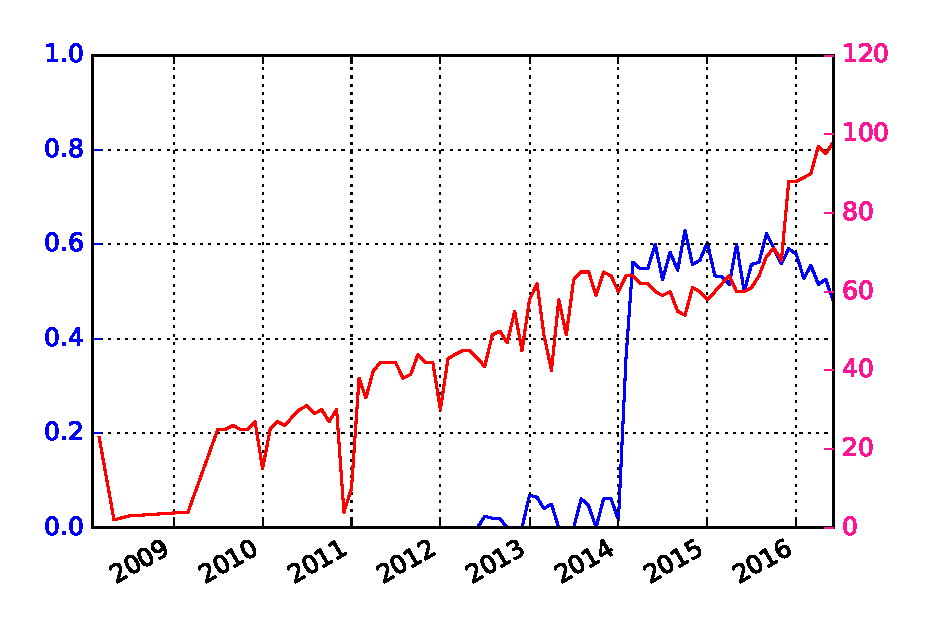
\includegraphics[width=.8\linewidth]{img/convergence_over_time_a}
		\caption{A-Root}
		\label{fig:ch04:convergence_a}
	\end{subfigure}
	\begin{subfigure}{.5\textwidth}
		\centering
		\includegraphics[width=.8\linewidth]{img/convergence_over_time_d}
		\caption{D-Root}
		\label{fig:ch04:convergence_d}
	\end{subfigure}
	\begin{subfigure}{.5\textwidth}
		\centering
		\includegraphics[width=.8\linewidth]{img/convergence_over_time_f}
		\caption{F-Root}
		\label{fig:ch04:convergence_f}
	\end{subfigure}
	\begin{subfigure}{.5\textwidth}
		\centering
		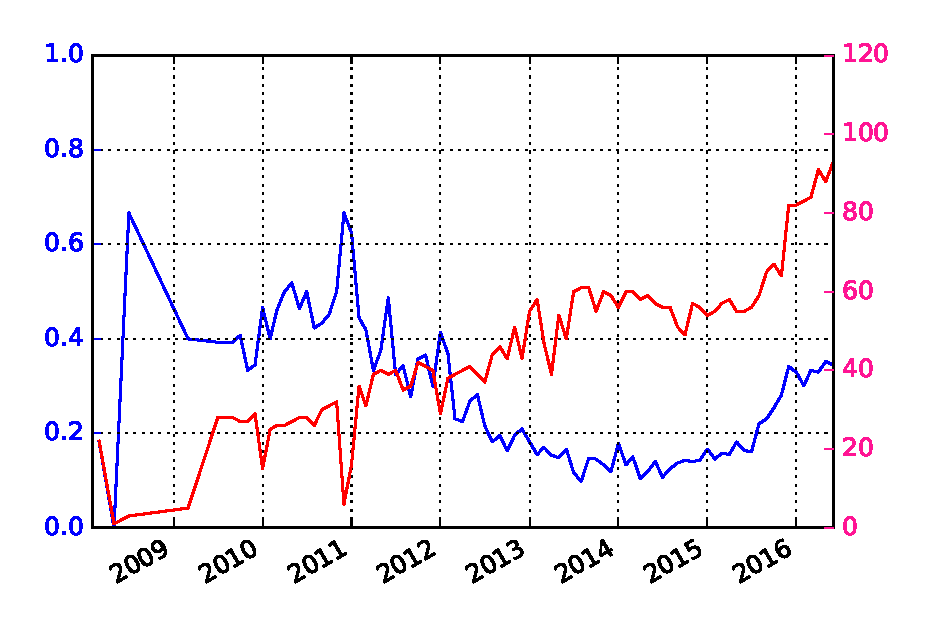
\includegraphics[width=.8\linewidth]{img/convergence_over_time_m}
		\caption{M-Root}
		\label{fig:ch04:convergence_m}
	\end{subfigure}	
	\caption{Convergence level of A, F, D, and M-Root. Results for others are available in Appendix \ref{app:convergence}}
	\label{fig:ch04:convergence}
\end{figure}

From the convergence graphs, a number of notable events can be noticed. Obviously, not all events can be explained since it requires the knowledge of complete routing policies implemented at the routers, which is not available in our datasets. Nevertheless, using the BGP routing data obtained from RIPEStat, some events can be explored as the following. 

\subsubsection{Dramatic Increase of A- and D-Root}
The common feature from A- (Figure \ref{fig:ch04:convergence_a}) and D-Root (Figure \ref{fig:ch04:convergence_d}) is that they experience dramatic increase at some point in time. 

A-Root is identified to have significant increase in February 2014. To analyze this, we compare data on January 1\textsuperscript{st} 2014 and February 1\textsuperscript{st} 2014. There are 60 and 64 dual-stacked VPs respectively, without any VP from January was absent in the subsequent month. Initially there was only one converging VP, then the number increased to 18 in February. 14 out of those 18 VPs converged due to the change in origin AS for IPv6 prefix (from AS 36623 to AS 36625). Recall from Section \ref{ch02:measuring-anycast} that A-Root originate their prefixes from multiple ASes, possibly one AS per instance\footnote{unfortunately, we cannot find official information available for confirmation}. One major factor contributing in low convergence level of A-Root is due to the difference of IPv4/IPv6 origin ASes as seen by VPs. For example, prior to January 2014, many VPs saw different origin ASes for IPv4 (AS 36625) and IPv6 (AS 36623). Later, IPv6-prefix announced by AS 36623 was withdrawn and originated by AS 36625, which resulted in convergence for VPs that already saw AS 36625 as the IPv4 origin AS. 

The sudden increase in D-Root is identified taking place at November 2013. Unlike A-Root, D-Root prefixes are originated from a single AS (AS 27) and the sudden increase is influenced by the changes in its upstream providers configuration. Initially, for IPv4 connectivity, D-Root is identified to have three upstream providers (AS 33657, AS 22925, and AS 10886) with AS 22925 as the main one. Then, around October 2013 D-Root was peered with another upstream provider (AS 42, Packet Clearing House), which immediately replaced AS 22925 to become the dominant upstream. As for IPv6, initially the most connections toward D-Root came through AS 10886. Then, AS 42 replaced its dominance as well. As the result, many diverging VPs that used to reach D-Root via different penultimate AS for IPv4 and IPv6 were switching to use AS 42 for both connectivities

By comparing BGP routing data on October  1\textsuperscript{st} and November  1\textsuperscript{st} 2013, there were 61 and 66 VPs respectively, without any VP in October became absent in November. There were only 4 converging VPs in October, and  significantly increased to 32 in the subsequent month. From those VPs in October that have diverging paths, 26 became convergent in November. All of them are because they used AS 42 as the penultimate AS of D-Root. Interestingly, all of them also experienced shorter paths than before. In fact, there were more VPs that switched to AS 42 for their IPv6 paths than their IPv4. To summarize, the decision to use AS 42 as the upstream provider for IPv4 and IPv6 significantly increases the convergence level and shorten the AS path length as well.

\subsubsection{Convergence Level Drops Experienced By F- and M-Root}
F- (Figure \ref{fig:ch04:convergence_f}) and M-Root (Figure \ref{fig:ch04:convergence_m}) experienced drops in their convergence level for some period of time. Since the number of VPs observing the prefixes fluctuate from time to time, it is rather difficult to observe a trend taking place in a period of time as opposed to, for example, sudden increase in A- and D-Root. Therefore, in this case study we select certain points of the trend and perform comparison on it. 

In F-Root case, we categorize it into two periods of drop: \textit{(i)} from July 2014 to December 2014, and \textit{(ii)} from December 2014 to November 2015. To make a comparable analysis, we seek VPs that present at the beginning and the end of each period. Afterwards, we only take VPs that changed its state from converging to diverging by the end of the period.

\begin{table}[!ht]
	\centering
	\begin{tabular}{c c c}
		\hline
		\textbf{VP} & \textbf{July 1\textsuperscript{st} 2014\tnote{a}}	& \textbf{December July 1\textsuperscript{st} 2014\tnote{b}} \\ \hline\hline
		\multirow{2}{*}{56730} & \texttt{\footnotesize [56730, 6939, 1280, 3557]}  & \texttt{\footnotesize [56730, 51945, 39326, 33073, 3557]} \\
		& \texttt{\footnotesize [56730, 6939, 1280, 3557]}  & \texttt{\footnotesize [56730, 6939, 1280, 3557]} \\ \hline
		
		\multirow{2}{*}{8607} & \texttt{\footnotesize [8607, 6939, 1280, 3557]}  & \texttt{\footnotesize [8607, 3257, 30132, 3557]} \\
		& \texttt{\footnotesize [8607, 6939, 1280, 3557]}  & \texttt{\footnotesize [8607, 6939, 1280, 3557]} \\ \hline
		
		\multirow{2}{*}{8758} & \texttt{\footnotesize [8758, 6939, 1280, 3557]}  & \texttt{\footnotesize [8758, 15576, 3257, 30132, 3557]} \\
		& \texttt{\footnotesize[8758, 6939, 1280, 3557]}  & \texttt{\footnotesize[8758, 6939, 1280, 3557]} \\ \hline
		
		\multirow{2}{*}{29636} & \texttt{\footnotesize [29636, 6939, 1280, 3557]}  & \texttt{\footnotesize [29636, 39326, 33073, 3557]} \\
		& \texttt{\footnotesize[29636, 6939, 1280, 3557]}  & \texttt{\footnotesize[29636, 6939, 1280, 3557]} \\ \hline
		
		\multirow{2}{*}{49605} & \texttt{\footnotesize [49605, 6939, 1280, 3557]}  & \texttt{\footnotesize [49605, 5580, 30132, 3557]} \\
		& \texttt{\footnotesize[49605, 6939, 1280, 3557]}  & \texttt{\footnotesize[49605, 6939, 1280, 3557]} \\ \hline
		
		\multirow{2}{*}{57821} & \texttt{\footnotesize [57821, 6939, 1280, 3557]}  & \texttt{\footnotesize [57821, 48039, 3257, 30132, 3557]} \\
		& \texttt{\footnotesize[57821, 6939, 1280, 3557]}  & \texttt{\footnotesize[57821, 6939, 1280, 3557]} \\ \hline
		
		\multirow{2}{*}{15605} & \texttt{\footnotesize [15605, 6939, 1280, 3557]}  & \texttt{\footnotesize [15605, 27320, 3557]} \\
		& \texttt{\footnotesize[15605, 6939, 1280, 3557]}  & \texttt{\footnotesize[15605, 6939, 1280, 3557]} \\ \hline
		
		\multirow{2}{*}{8447} & \texttt{\footnotesize [8447, 6939, 1280, 3557]}  & \texttt{\footnotesize [8447, 30132, 3557]} \\
		& \texttt{\footnotesize[8447, 6939, 1280, 3557]}  & \texttt{\footnotesize[8447, 6939, 1280, 3557]} \\ \hline\hline
		
		\textbf{VP} & \textbf{December 1\textsuperscript{st} 2014}	& \textbf{November 1\textsuperscript{st} 2015} \\ \hline\hline
		\multirow{2}{*}{22548} & \texttt{\footnotesize [22548, 30122, 3557]}  & \texttt{\footnotesize [22548, 30122, 3557]} \\
		& \texttt{\footnotesize [22548, 30122, 3557]}  & \texttt{\footnotesize [22548, 16735, 27781, 28054, 3557]} \\ \hline
		
		\multirow{2}{*}{52888} & \texttt{\footnotesize [52888, 30122, 3557]}  & \texttt{\footnotesize [52888, 30122, 3557]} \\
		& \texttt{\footnotesize [52888, 30122, 3557]}  & \texttt{\footnotesize [52888, 1916, 6939, 27781, 28054, 3557]} \\ \hline
		
		\multirow{2}{*}{16735} & \texttt{\footnotesize [16735, 22548, 30122, 3557]}  & \texttt{\footnotesize [16735, 22548, 30122, 3557]} \\
		& \texttt{\footnotesize [16735, 22548, 30122, 3557]}  & \texttt{\footnotesize [16735, 27781, 28054, 3557]} \\ \hline
		
		\multirow{2}{*}{14840} & \texttt{\footnotesize [14840, 30122, 3557]}  & \texttt{\footnotesize [14840, 30122, 3557]} \\
		& \texttt{\footnotesize [14840, 30122, 3557]}  & \texttt{\footnotesize [14840, 18881, 3549, 6939, 27781, 28054, 3557]} \\ \hline
		
		\multirow{2}{*}{1916} & \texttt{\footnotesize [1916, 30122, 3557]}  & \texttt{\footnotesize [1916, 30122, 3557]} \\
		& \texttt{\footnotesize [1916, 30122, 3557]}  & \texttt{\footnotesize [1916, 6939, 27781, 28054, 3557]} \\ \hline
	\end{tabular}
	\begin{tablenotes}
		\item For each VP, the upper and lower rows represents IPv4 and IPv6 AS paths, respectively
	\end{tablenotes}
	\caption{Diverging VPs of F-Root during two periods of level drop}
	\label{table:ch04:convergence:f-root-analysis}
\end{table}

Table \ref{table:ch04:convergence:f-root-analysis} presents the selected VPs for each period. It can be seen that in the beginning of the first period (July 1\textsuperscript{st} 2014), all diverging VPs reached F-Root through upstream AS 1280 for both IPv4 and IPv6. Diverging VPs in the end of the first period (December 1\textsuperscript{st} 2014) are due to the change of IPv4 penultimate AS, \textit{i.e.}, from 1280 to any other. The second period is similar to the first one, except that now it is caused by F-Root instance identified by AS 30122 instead of AS 1280. In contrast to the first period, now the divergence happens due to the change of penultimate AS in IPv6 route (from AS 30122 to 28504). 

Recall from Section \ref{ch02:anycast} that F-Root uses unique penultimate AS for each of its instance for physical identifier at control-plane level, while originating their prefixes from a single AS. It means that those diverging VPs in Table \ref{table:ch04:convergence:f-root-analysis} are directed toward different instances for IPv4 and IPv6. 
Based on PeeringDB data\footnote{\url{https://www.peeringdb.com/asn/1280}}, we believe that AS 1280 is the identifier for F-Root global nodes. Therefore, in the first period, the VPs switched from the global nodes to other local instances.  By the end of the period, most of them used F-Root local instance in London (identified by AS 33073), while the rest went to the Netherlands (identified by AS 30132). F-Root global nodes are located in United States, and one in Amsterdam. All of these VPs are located in Europe (Milan, Vienna, Amsterdam, and mostly in London). However, their IPv6 route still used the global instance. 

Stranger case is identified in the second period. Initially, the VPs in second period (all of them are located in Sao Paulo, Brazil) chose F-Root instance in Sao Paulo (identified by AS 30122) for both IPv4 and IPv6, which is the ideal scenario. However, they later identified to switch using the instance in Sint Marteen, Anguilla  (identified by AS 28054), which located in Carribean for IPv6 connection. Both instances are configured as local nodes. The fact that those Sao Paulo VPs saw and selected Carribean instance indicates either Sao Paulo instance's IPv6 service was offline and Sint marteen instance's catchment area was intentionally configured to cover Sao Paulo, or simply route leakage happened during that interval.

\begin{table}[!ht]
	\centering
	\begin{tabular}{c c c}
		\hline
		\textbf{VP} & \textbf{Feb 1$^{st}$ 2012}	& \textbf{Apr 1$^{st}$ 2014} \\ \hline\hline
		\multirow{2}{*}{680} & \texttt{\footnotesize [680, 20965, 2200, 7500]}  & \texttt{\footnotesize [680, 20965, 11537, 22388, 7660, 2500, 7500]} \\
		& \texttt{\footnotesize [680, 20965, 2200, 7500]}  & \texttt{\footnotesize [680, 20965, 2200, 7500]} \\ \hline
		
		\multirow{2}{*}{9002} & \texttt{\footnotesize [9002, 2497, 7500]}  & \texttt{\footnotesize [9002, 2497, 7500]} \\
		& \texttt{\footnotesize [9002, 2497, 7500]}  & \texttt{\footnotesize [9002, 6939, 7500]} \\ \hline
		
		\multirow{2}{*}{12859} & \texttt{\footnotesize [12859, 3257, 7500]}  & \texttt{\footnotesize [12859, 3257, 7500]} \\
		& \texttt{\footnotesize[12859, 3257, 7500]}  & \texttt{\footnotesize[12859, 6939, 7500]} \\ \hline
		
		\multirow{2}{*}{1853} & \texttt{\footnotesize [1853, 20965, 2200, 7500]}  & \texttt{\footnotesize [1853, 3356, 2516, 7500]} \\
		& \texttt{\footnotesize[1853, 20965, 2200, 7500]}  & \texttt{\footnotesize[1853, 6939, 7500]} \\ \hline
		
		\multirow{2}{*}{1103} & \texttt{\footnotesize [1103, 20965, 2200, 7500]}  & \texttt{\footnotesize [1103, 2603, 11537, 22388, 7660, 2500, 7500]} \\
		& \texttt{\footnotesize[1103, 20965, 2200, 7500]}  & \texttt{\footnotesize[1103, 20965, 2200, 7500]} \\ \hline
		
		\multirow{2}{*}{29140} & \texttt{\footnotesize [29140, 3257, 7500]}  & \texttt{\footnotesize [29140, 3257, 7500]} \\
		& \texttt{\footnotesize[29140, 3257, 7500]}  & \texttt{\footnotesize[29140, 6939, 7500]} \\ \hline\hline
		
		\textbf{VP} & \textbf{April 1$^{st}$ 2014}	& \textbf{June 1$^{st}$ 2016} \\ \hline\hline
		\multirow{2}{*}{48166} & \texttt{\footnotesize [48166, 12389, 2516, 7500]}  & \texttt{\footnotesize [48166, 7500]} \\
		& \texttt{\footnotesize [48166, 6939, 7500]}  & \texttt{\footnotesize [48166, 7500]} \\ \hline
		
		\multirow{2}{*}{31019} & \texttt{\footnotesize [31019, 41887, 5580, 2497, 7500]}  & \texttt{\footnotesize [31019, 7500]} \\
		& \texttt{\footnotesize [31019, 6939, 7500]}  & \texttt{\footnotesize [31019, 7500]} \\ \hline
		
		\multirow{2}{*}{12859} & \texttt{\footnotesize [12859, 3257, 7500]}  & \texttt{\footnotesize [12859, 7500]} \\
		& \texttt{\footnotesize [12859, 6939, 7500]}  & \texttt{\footnotesize [12859, 7500]} \\ \hline
		
		\multirow{2}{*}{15435} & \texttt{\footnotesize [15435, 3257, 7500]}  & \texttt{\footnotesize [15435, 7500]} \\
		& \texttt{\footnotesize [15435, 6939, 7500]}  & \texttt{\footnotesize [15435, 7500]} \\ \hline
		
		\multirow{2}{*}{29140} & \texttt{\footnotesize [29140, 3257, 7500]}  & \texttt{\footnotesize [29140, 3257, 7500]} \\
		& \texttt{\footnotesize [29140, 6939, 7500]}  & \texttt{\footnotesize [29140, 3257, 7500]} \\ \hline
		
		\multirow{2}{*}{12779} & \texttt{\footnotesize [12779, 174, 3257, 7500]}  & \texttt{\footnotesize [12779, 7500]} \\
		& \texttt{\footnotesize [12779, 6939, 7500]}  & \texttt{\footnotesize [12779, 7500]} \\ \hline
		
		\multirow{2}{*}{34288} & \texttt{\footnotesize [34288, 3257, 7500]}  & \texttt{\footnotesize [34288, 7500]} \\
		& \texttt{\footnotesize [34288, 6939, 7500]}  & \texttt{\footnotesize [34288, 7500]} \\ \hline				
	\end{tabular}
	\begin{tablenotes}
		\item For each date, the upper and lower row represents IPv4 and IPv6 AS path, respectively
	\end{tablenotes}
	\caption{Decreasing (February 2012--April 2014) and increasing (April 2014--June 2016) period of convergence level experienced by M-Root}
	\label{table:ch04:convergence:m-root-analysis}
\end{table}

Now let us discuss M-Root. M-Root has decreasing and later increasing periods of convergence level (Figure \ref{fig:ch04:convergence_m}). Using similar method used to analyze F-Root, we obtain result in Table \ref{table:ch04:convergence:m-root-analysis}. For the decreasing period, it seems to be caused by different transit AS used to reach M-Root. Two VPs were switched from AS 2200 to AS 2500 for IPv4, which also results in much longer AS path. For the rest, the change is in IPv6 transit AS, where the converging VPs switched to access M-Root via AS 6939 later. For the converging period, the increase of convergence level is partly caused by network expansion of M-Root. It can be seen that previously M-Root have different routing policy for IPv4 and IPv6, with AS 6939 is mainly used as the IPv6 upstream. Later, M-Root decided to make direct peering sessions with many other ASes for both IPv4 and IPv6, resulting in shorter (and converging) AS path. 

\subsubsection{Why Do M- and J-Root Have The Worst Convergence Level?}

Compared to the others, J- and M-Root have the worst convergence level. For J-Root, it is easily understood. J-Root is similar to A-Root in the sense that they also use multiple ASes to announce their prefixes\footnote{As opposed to A-Root that can be inferred that each AS represents an instance, J-Root seems to group together multiple instances into different origin ASes. Unfortunately, we cannot find official information regarding their anycast configuration.}. Thus, diverging paths due to different origin ASes experienced by a VP can be easily detected, unlike anycast service that uses a single origin AS. However, A-Root have better convergence level than J-Root. We believe that it is because A-Root only has five instances where all of them are global nodes and dual-stacked, compared to 112 J-Root instances with only 12 of them are dual-stacked. Thus, VPs located outside of the catchments of those 12 dual-stacked instances are likely to have diverging paths. Of all diverging VPs throughout the observation period, 57.8\% is caused by different IPv4/IPv6 origin ASes. However, it is not just merely about the number of dual-stacked instances. Take J-Root as an example. From all of its dual-stacked instances, half of them are located in the same cities as some of RIS collectors. However, it does not automatically translate to better reachability from VP's point of view. %For instance, collectors in Amsterdam still experience different paths (Figure \ref{fig:coll-ams-ix} and \ref{fig:coll-ripe-ncc}).

\begin{figure}
%	\begin{subfigure}{1\textwidth}
%		\centering
%		\includegraphics[width=5.0in]{img/j_root_top_upstream.png}
%		\caption{J-Root's most dominant upstream providers}
%		\label{fig:ch04:j_root_top_upstream}
%	\end{subfigure}
%	\begin{subfigure}{1\textwidth}
		\centering
		\includegraphics[width=5.0in]{img/m_root_top_upstream.png}
%		\caption{M-Root's most dominant upstream providers}
%		\label{fig:ch04:m_root_top_upstream}
%	\end{subfigure}	
	\caption{M-Root's most dominant upstream providers }
	\label{fig:ch04:top_upstream}
\end{figure}

In contrast to J-Root, M-Root only has five instances where all of them are global nodes and dual-stacked. Low convergence level of M-Root is caused by different routing policies for IPv4 and IPv6 that prefer certain providers to transit. Figure \ref{fig:ch04:top_upstream} illustrates M-Root's top upstream providers as seen by RIS collectors. Since 2011, AS 6939 (Hurricane Electric) has been dominating M-Root's IPv6 upstream (more than 50\%). On the other hand, the IPv4 connectivities are more distributed among several transit providers/peers. The top IPv4 upstream providers are AS 3257 and AS 24785, which are not as dominant as AS 6939 in IPv6. Thus, low convergence level in M-Root case is due to different upstream providers used to reach M-Root.

\subsubsection{Visibility of Root Servers}

As explained in the beginning of this section, Appendix \ref{app:convergence} can also be used to understand the visibility of Root Servers as seen by VPs. %While the nominal is varying for each Root Server, the red line patterns are roughly similar for all, indicating that the number of BGP routers participating in RIS project keeps growing over the time. 
High number of dual-stacked VPs means high level of visibility, or in another word, larger catchment area. The number of VPs are increasing over the time, which is in line with the expansion of the deployed collectors. This is especially noticeable by the end of 2015, where the figure is significantly increased due to the addition of new collectors (Table \ref{table:ch03:ris-collectors}). Ideally, all Root Servers should have relatively similar red line height for a given time, meaning that a similar number of VPs have exposure to those Root Servers. This is not what happens in practice, of course, due to different policies implemented by the operators (amount of deployed instances and its placement, peering agreements, and so on).  
% the nominal of dual-stacked VPs means IPv4 and IPv6 visibility as seen by VPs. The question is, how many VPs that have IPv4 route but not IPv6, and vice versa? don't you think it is more appropriate to represent the visibility?

Large number of instances supposedly should directly correlate to high visibility, while the amount of dual-stacked instances does not have contribution here since the VPs may take any path towards the instances as long as the instances are configured as global nodes. However, this does not always apply. Root Servers with small number of instances (\textless 10)--A, C, and M-Root--have relatively high level of visibility. The lowest ones are F and I-Root, even though both of them have \textasciitilde50 instances. More interestingly, all I-Root instances are configured as global nodes, which should have provided higher exposure to the global Internet. 

We believe that the reason is because F- and I-Root are lacking of peering connection with large providers that are willing to provide global visibility. A- and C-Root are operated by commercial organizations (Verisign and Cogent, respectively) that run large-scale network infrastructures globally. It allows them to provide better connectivities with the rest of the Internet. M-Root peers with a number of of ISPs, with some of them provide free transit service\footnote{\url{http://m.root-servers.org/}}. On the other hand, F- and I-Root use open peering policy that requires participation from the interested organizations. Free peering sessions are typically used to exchange traffic between each others'networks, but not to reach the rest of the Internet. Thus, it limits the visibility of the Root Servers beyond its peers. However, K-Root also implements the same policy but with larger visibility level. We believe that this is due to the status of RIPE as the operator of K-Root, which have large base of membership in its region. Hence, it is easier for RIPE to promote direct peering between K-Root instances and RIPE members.

%In F-Root case, from five of its global nodes, four of them are located in United States, and one is in Amsterdam. 


\subsection{The Trends of AS Path Lengths}
\label{ch04:evolution:as-path-length}
%Dhamdhere et al. \cite{Dhamdhere:2012:MDI:2398776.2398832} concluded that the overall AS path length for IPv6 shows a decreasing trend, and showed sharp decreasing since 2008. As for IPv4, the average AS path length is stable around 4 AS hops.
Appendix \ref{app:path-avg:all-peers} provides the statistics of AS path lengths of VPs toward all selected Root Servers over the observation period. The green line on all graphs illustrates the median of path length, which is summarized in Table \ref{table:ch04:path-length-average}. Except for A and D-Root, Root Servers do not experience much changes on their path lengths over the time. 

Past study shows that the average AS path length tends to get shorter, especially for IPv6  \cite{update}. This is further confirmed by Dhamdhere et al. \cite{Dhamdhere:2012:MDI:2398776.2398832}, who concluded that the overall AS path length for IPv6 shows a decreasing trend, and showed sharp decreasing since 2008. As for IPv4, the average AS path length is stable around 4 AS hops. Result from this thesis indicates roughly similar figure. In general, the average IPv4 and IPv6 path length is marginally less than 4, with the difference between them is not significant. Compared to the rest, K-Root has the shortest path length for both IPv4 and IPv6. It generally shows that K-Root has better reachability as seen by VPs. On the other hand, I-Root have the longest average path length, albeit not that significantly different with the rest. 

Overall, the difference between IPv4 and IPv6 path lengths for each Root Server is not that much. However, convergence level seems to have effect on it. Root Servers with poor convergence level (M- and J-Root) have the highest differences. J-Root have noteworthy lower IPv4 path length compared to its IPv6. On the contrary, M-Root have prominently lower IPv6 path length than its IPv4. It shows that J and M-Root have stronger connectivity on either protocol.

\begin{figure}
	\begin{subfigure}{1\textwidth}
		\centering
		\includegraphics[width=6.5in]{img/path_avg_all_d.png}
		\caption{AS path lengths of D-Root}
		\label{fig:ch04:trends_avg_path_length_d}
	\end{subfigure}
	\begin{subfigure}{1\textwidth}
		\centering
		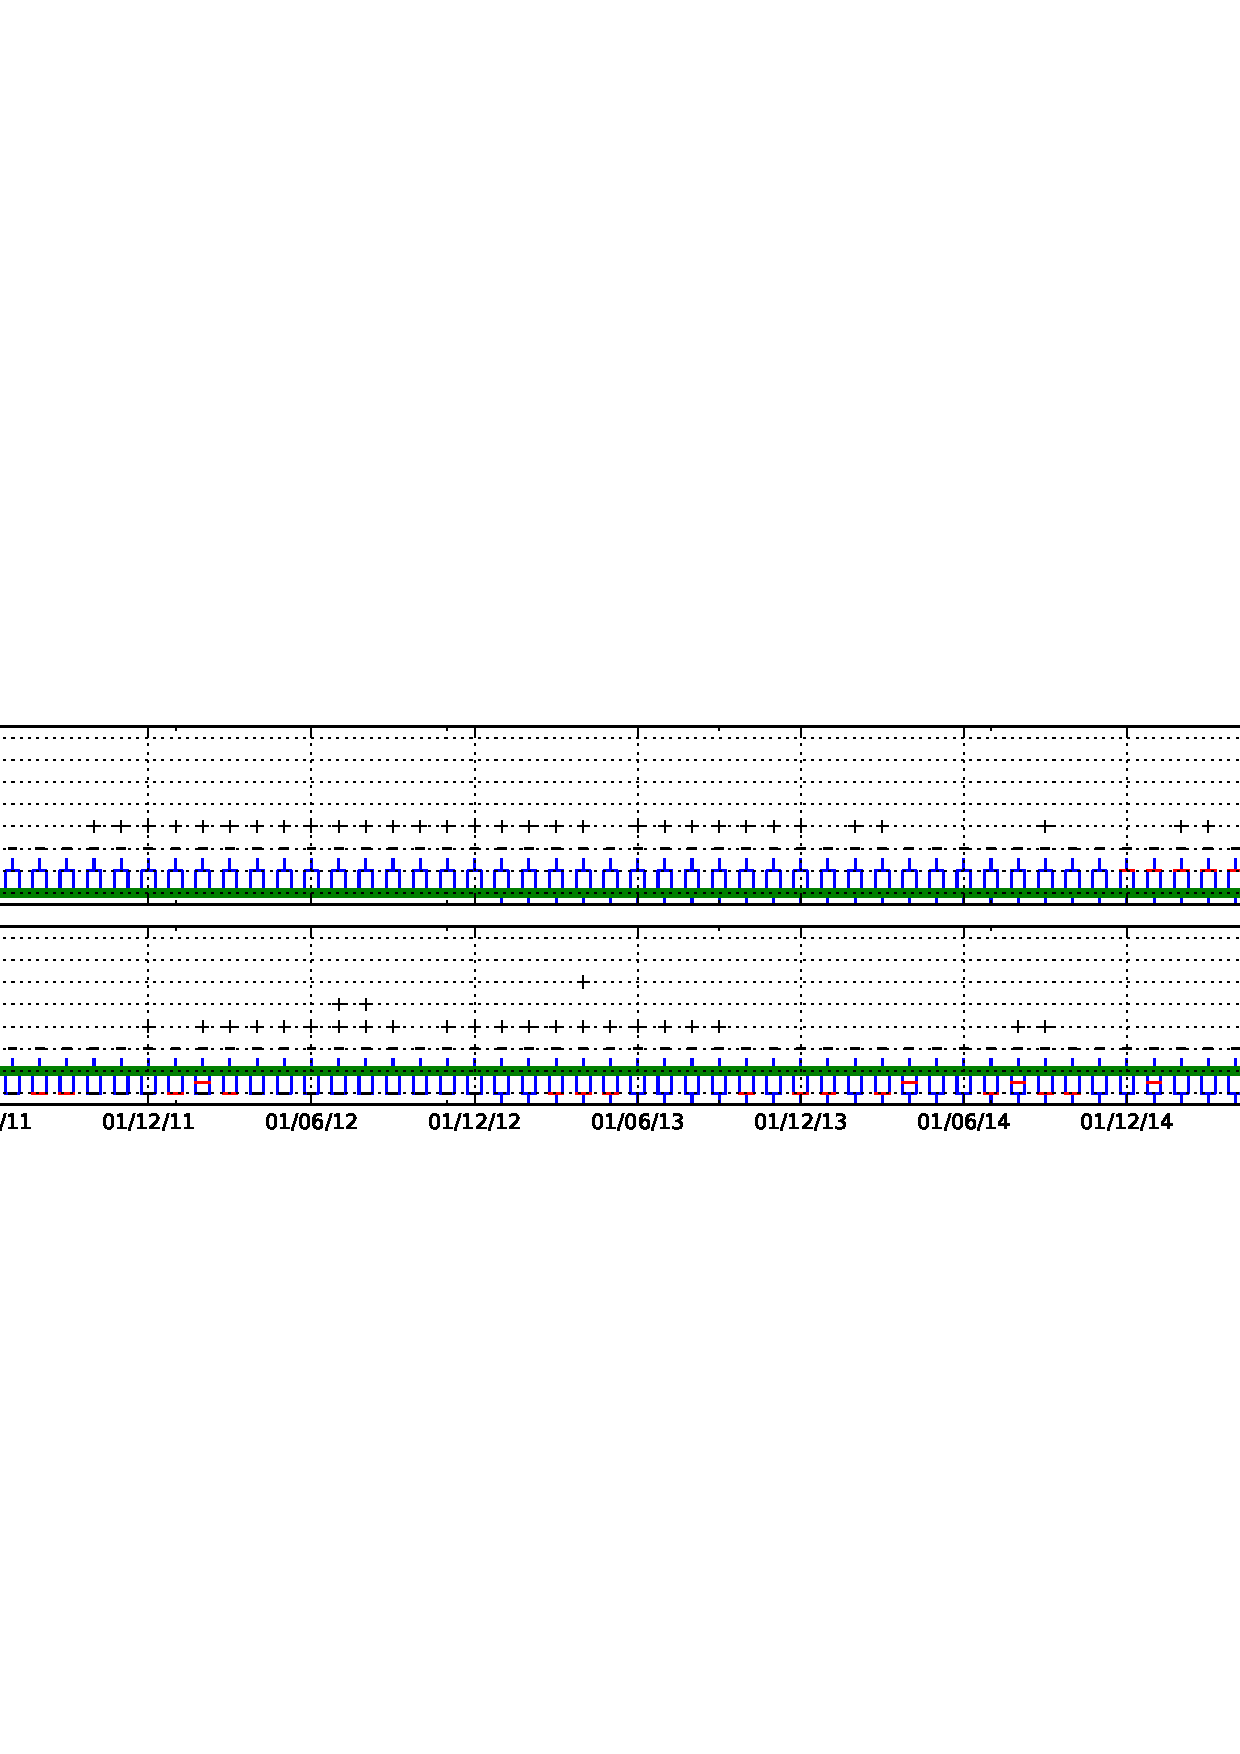
\includegraphics[width=6.5in]{img/path_avg_all_k.png}
		\caption{AS path lengths of K-Root}
		\label{fig:ch04:trends_avg_path_length_k}
	\end{subfigure}
	\begin{subfigure}{1\textwidth}
		\centering
		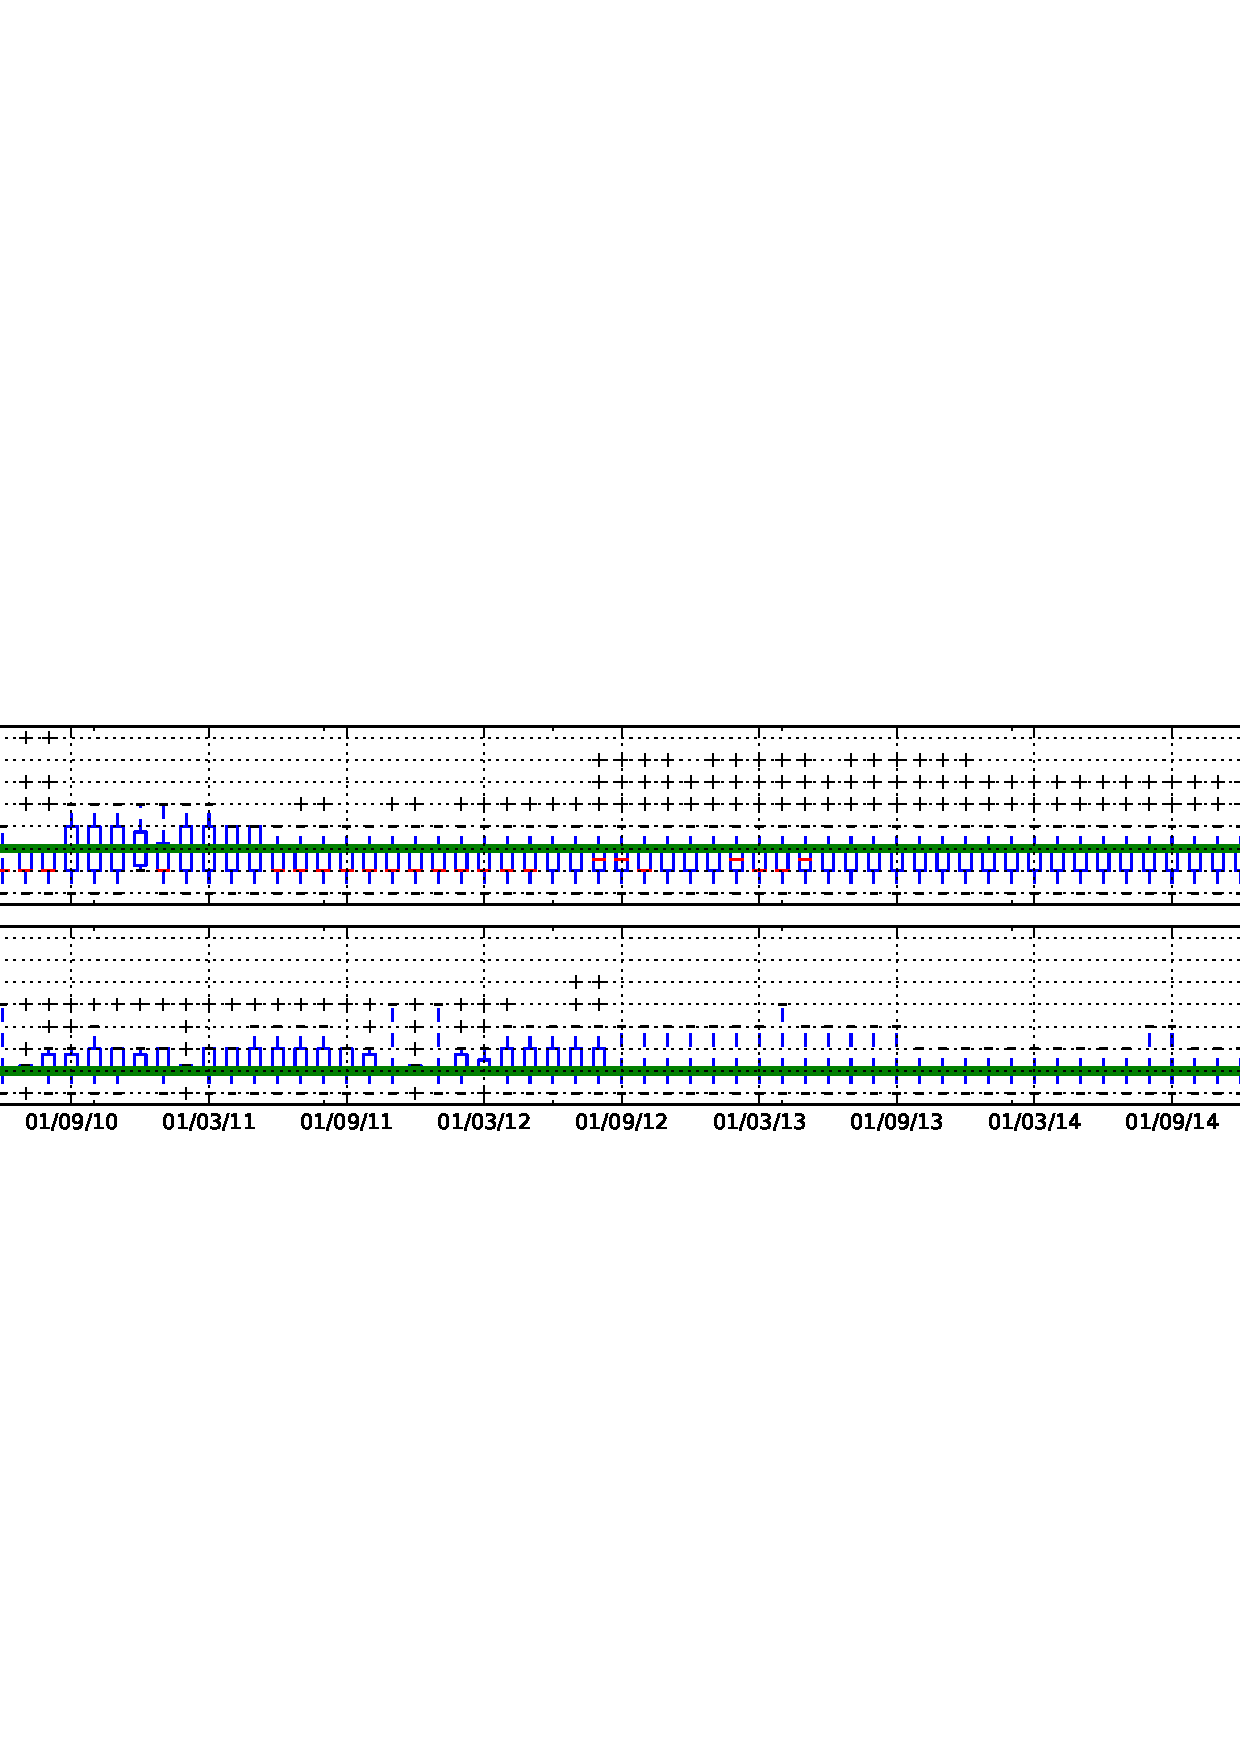
\includegraphics[width=6.5in]{img/path_avg_all_m.png}
		\caption{AS path lengths of M-Root}
		\label{fig:ch04:trends_avg_path_length_m}
	\end{subfigure}
	{\scriptsize \\These are the box plots which represent the distribution of AS path lengths of the respective Root Servers. The central rectangle comprises of three parallel horizontal lines representing the first quartile, the median (red), and the third quartile. The whisker below the rectangle represents the minimum value, while the top whisker is the maximum one. The outlier data is depicted as crosses. The green line represents the average of the median over the time\par}
	\caption{AS path lengths of D, K, and M-Root}
	\label{fig:ch04:trends_avg_path_length}
\end{figure}

%Figure \ref{fig:ch04:trends_avg_path_length} represents selected graphs from Appendix \ref{app:path-avg:all-peers}. D-Root (Figure \ref{fig:ch04:trends_avg_path_length_d}) looks to have two phases of path length dynamism (pre- and post-November 2013), and it will be discussed later. K-Root (Figure \ref{fig:ch04:trends_avg_path_length_k}) 

\begin{table}[!ht]
	\centering
	\begin{tabular}{c c c c c}
		\hline
		\multirow{2}{*}{\textbf{Root Server}} & \multicolumn{2}{c}{\textbf{Median}} & \multicolumn{2}{c}{\textbf{Mean}} \\
		& \textbf{IPv4} & \textbf{IPv6} & \textbf{IPv4} & \textbf{IPv6} \\
		%\textbf{Root Server} & \textbf{IPv4}	& \textbf{IPv6} \\ 
		\hline\hline
		A			& 4 & 3 & 3.79	& 3.64 \\ \hline
		C			& 4 & 4 & 3.68	& 3.77 \\ \hline
		D			& 4 & 4 & 3.78	& 3.75 \\ \hline
		F			& 4 & 4 & 3.65	& 3.67 \\ \hline
		I			& 4 & 4 & 3.86	& 3.90 \\ \hline
		J			& 3 & 3 & 3.18	& 3.62 \\ \hline
		K			& 2 & 3 & 2.56	& 2.65 \\ \hline
		L			& 3 & 3 & 2.95	& 3.03 \\ \hline
		M			& 4 & 3 & 3.68	& 3.10 \\ \hline
	\end{tabular}
	\caption{Median and mean of IPv4 and IPv6 path lengths over the time}
	\label{table:ch04:path-length-average}
\end{table}


Appendix \ref{app:path-avg:all-peers} can be used to see the stability of the AS path length over the time as well.  C, K, and L-Root are relatively stable. It means that there was not major network configuration changes affecting the path length from the VPs. D-Root (Figure \ref{fig:ch04:trends_avg_path_length_d}) looks to have two phases of its path length dynamics. The fluctuated path length of D-Root VPs started to stabilize at November 2013, the same time when D-Root started to use AS 42 as one of their upstream (Section \ref{ch04:evolution:convergence}). This decision seemed to help D-Root gaining lower average path lengths than before, and since then the path length did not vary much. M-Root IPv6 path length (Figure \ref{fig:ch04:trends_avg_path_length_m}) looks similar to D-Root. Starting from September 2012, the path lengths started to stabilize. IPv6 path lengths of M-Root's VPs are mostly 3 (indicated by flat rectangle at 3), which shows that they use an upstream provider that have large connectivities, which is AS 6939 (Figure \ref{fig:ch04:top_upstream}). For A-Root, the path lengths were highly varying until the beginning of 2014, when the length started to stabilize. We believe that the discussion of A-Root in Section \ref{ch04:evolution:convergence} also takes part in this dynamics.

The graphs in Appendix \ref{app:path-avg:all-peers} also inform us about the symmetry of the catchment topology. Ideally, an anycast catchment topology should be in the form of tree(s) where the origin AS of anycast service serves as the center of tree (or their upstream provider(s)), and all end-user ASes should have relatively similar path lengths. It demonstrates that the anycast instances provide good reachability from any corner of the Internet, and that the instances are properly distributed. Quantitatively, this behavior is indicated by a box plot with narrow range of upper and lower whiskers, and as few outliers as possible. C-Root (Figure \ref{fig:path-avg-all-c}) is a good example of it. The extreme contrasting example is M-Root's IPv4 path length. M-Root's poor IPv4 statistics compared to its IPv6 is not because of the overall poor connectivities, but largely contributed by small number of VPs that have quite long paths (marked as outliers in Figure \ref{fig:path-avg-all-m}). It may serve a good indicator on planning new peering agreement or even new instance deployment to provide better connectivities.  



\section{The Differences Between IPv4 and IPv6 Catchment Areas}
\label{ch04:differences}
Previous section discusses about the dynamics of anycast catchment areas over the time in terms of the convergence level and the trends of AS path length. It uses data from all VPs as long as they have both IPv4 and IPv6 routing information toward Root Server. In this section, we focus our discussion on the differences between IPv4 and IPv6 catchment areas itself. Therefore, we focus only on diverging VPs of certain Root Server at a given time. The definition of different AS paths used in this thesis is provided in Section \ref{ch03:analysis}. With current data we have in our disposal, we can not answer the question of \textit{why} exactly the differences take place, since it requires the knowledge of BGP routing configuration on each routers. However, we can find out \textit{to what extent} the differences affecting the catchment areas, as seen from control-plane perspective. 

We start off by discussing the composition of VPs (Section \ref{ch04:diff:composition}). Next, the average path length (Section \ref{ch04:diff:avg-path-length}), followed by how different is it path-length-wise (Section \ref{ch04:diff:diff-how-diff}).

\subsection{Composition of VPs}
\label{ch04:diff:composition}

Different paths encountered by a diverging VP may still result in similar path lengths, or it could also result in either IPv4 or IPv6 shorter path. Section \ref{ch04:evolution:convergence} specifically focuses  on the fraction of converging VPs of all dual-stacked VPs. Here, we are interested to look deeper at the diverging VPs: how many diverging VPs that experience shorter IPv4 path, shorter IPv6 path, or similar path lengths. By breaking down the composition of all VPs based on its IPv4/IPv6 path lengths, we present the results in Appendix \ref{app:peer-composition} with Figure \ref{fig:ch04:composition} showing composition of A and D-Root's VPs serves as an example. Root Servers have more diverging VPs with equal IPv4/IPv6 path lengths than shorter IPv4/IPv6 path, except for J, I, and M-Root. I-Root itself has slightly more diverging VPs with shorter IPv6 paths. Root Servers with low convergence level (J and M-Root) have noticable shorter paths. J-Root is dominated by VPs with shorter IPv4 path. On the contrary, VPs with shorter IPv6 path dominate M-Root.
 

\begin{figure}[!ht]
	\begin{subfigure}{1\textwidth}
		\centering
		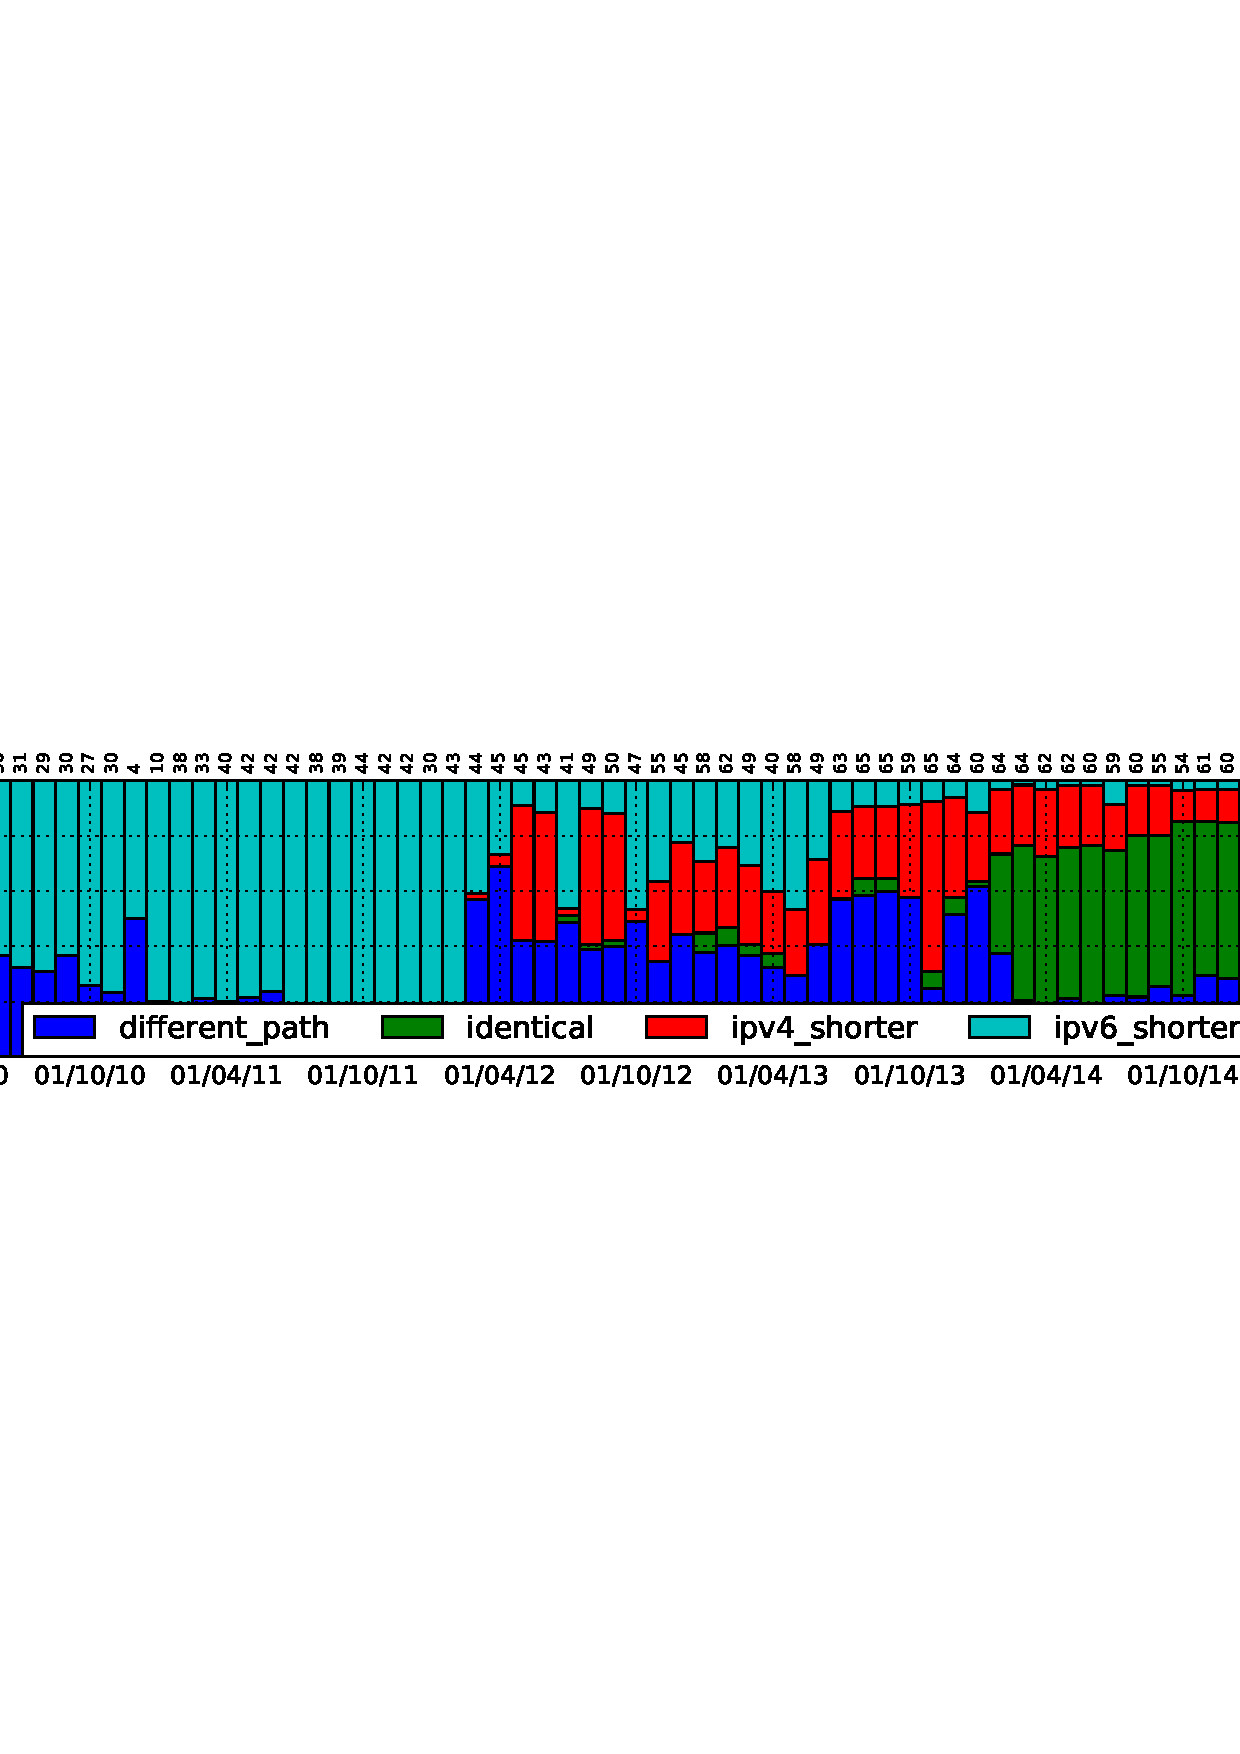
\includegraphics[width=6in]{img/peer_composition_a.png}
		\caption{Composition of A-Root's VPs}
		\label{fig:ch04:composition_a}
	\end{subfigure}
	\begin{subfigure}{1\textwidth}
		\centering
		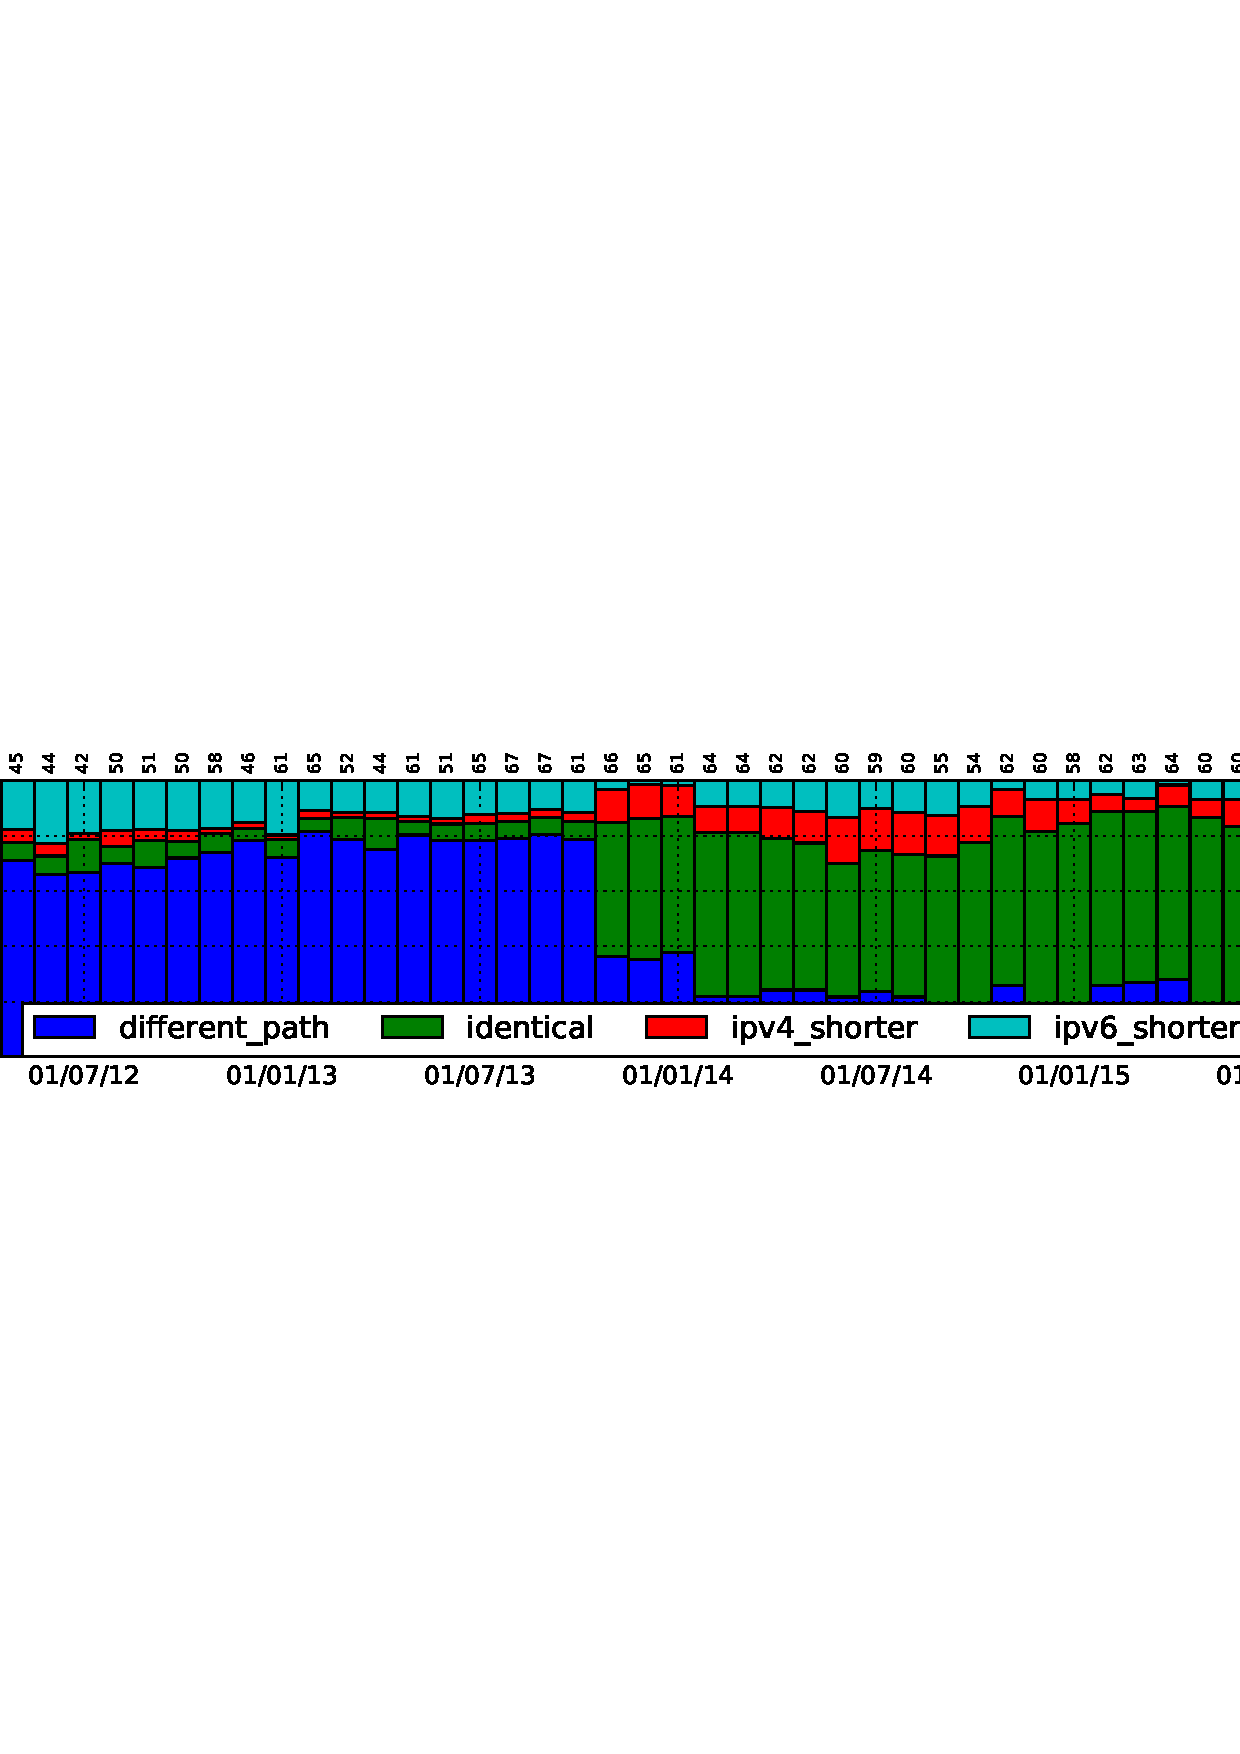
\includegraphics[width=6in]{img/peer_composition_d.png}
		\caption{Composition of D-Root's VPs}
		\label{fig:ch04:composition_d}
	\end{subfigure}	
	{\scriptsize The bins represent the fraction of VPs for each category. The number on top of the bin shows the total number of VPs at a time}
	\caption{Composition of A and D-Root's VPs}
	\label{fig:ch04:composition}
\end{figure}


Diverging paths with equal lengths is largely due to coincidence. However, there are some special cases, for example in D-Root (Figure \ref{fig:ch04:composition_d}). It has large fraction of VPs with diverging path and equal length prior to November 2013. We have discussed in Section \ref{ch04:evolution:convergence} that prior to November 2013, the dominant upstream was AS 22945. AS 22945 itself is identified to have all connectivities by transiting via AS 6939.
The similar case also happens in IPv6, now with AS 10886 as the upstream. In D-Root case, VPs with diverging paths and equal length prior to November 2013 mostly happened because the VPs reached D-Root through AS 22945 for IPv4 and through AS 10886 for IPv6, with AS 6939 as the intermediate transit AS. VPs path via AS 6939 were always the same (regardless IPv4/IPv6), the only difference is the penultimate AS before reaching D-Root's origin AS. After the introduction of AS 42, the catchment topology changed, since most VPs switched to reach D-Root via AS 42.

Prior to February 2012, A-Root (Figure \ref{fig:ch04:composition_a}) was dominated by VPs with shorter IPv6 paths. It is because A-Root directly peered with AS 6939 and all IPv6 connectivities were through them. This is also one of the reasons why A-Root had such low convergence level during that period, as AS 6939 is the dominant IPv6 transit provider thus A-Root's VPs experienced shorter IPv6. Starting in March 2012, they started to use other IPv6 transit providers as well, resulting in the VPs no longer got shorter IPv6. We believe that this event lead to higher A-Root IPv6 path lengths starting from march 2012 in Figure \ref{fig:path-avg-all-a}.

\subsection{Average Path Length}
\label{ch04:diff:avg-path-length}

We have discussed the trends of AS path lengths for all VPs in Section \ref{ch04:evolution:as-path-length}. Here, we focus only on average path length of diverging VPs. The complete result is presented in Appendix \ref{app:path-avg:diff-paths}, and summarized in Table \ref{table:ch04:path-length-average-diff}. To get the knowledge of the quantity of VPs for each AS path lengths, we break down the data to get the VPs degree (relative to the Root Server) in Appendix \ref{app:peer-degree-dist}. 

Intuitively, the longer the path the higher the probability of having diverging paths is. In general, the results in Appendix \ref{app:path-avg:diff-paths} exhibit similar patterns with the ones in Appendix \ref{app:path-avg:all-peers}. This is because of two factors: \textit{(i)} the number of diverging VPs are not significant to influence the overall path length distribution, \textit{(ii)} diverging VPs are generally have longer paths, but not that much, as we see later. Comparing results in Table \ref{table:ch04:path-length-average-diff} and Table \ref{table:ch04:path-length-average}, we see that Root Servers with high convergence level, especially C-, I-, and K-Root, have the largest differences. This is especially noticeable for C-Root, the one with the highest differences (0.53 hop for IPv4 and 0.76 hop for IPv6) by comparing Figure \ref{fig:path-avg-all-c} and Figure \ref{fig:path-avg-diff-c}. The contrast of C-Root's average path lengths between all dual-stacked VPs and diverging VPs only are depicted in Figure \ref{fig:ch04:peer_degree_c}.
Root Servers with low convergence level, J- and M-Root, only slightly differ because the diverging VPs dominate the statistics in Table \ref{table:ch04:path-length-average}. It means that the diverging VPs mostly have longer AS path lengths than the average, thus confirming the hypothesis.

\begin{figure}[!ht]
	\centering
	\begin{subfigure}{1\textwidth}
		\centering
		\includegraphics[width=6.5in]{img/peer_degree_all_c.png}
		\caption{All dual-stacked VPs}
		\label{fig:ch04:peer_degree_all_c}
	\end{subfigure}
	\begin{subfigure}{1\textwidth}
	\includegraphics[width=6.5in]{img/peer_degree_diff_c.png}
	\caption{Diverging VPs only}
	\label{fig:ch04:peer_degree_diff_c}
	\end{subfigure}	
	{\scriptsize The bins represent the fraction of VPs for each category. The number on top of the bin shows the total number of VPs at a time}
	\caption{C-Root's VP degree}
	\label{fig:ch04:peer_degree_c}
\end{figure}
 

\begin{table}[!ht]
	\centering
	\begin{tabular}{c c c c c}
		\hline
		%\textbf{Root Server} & \textbf{IPv4}	& \textbf{IPv6} \\ \hline\hline
		\multirow{2}{*}{\textbf{Root Server}} & \multicolumn{2}{c}{\textbf{Median}} & \multicolumn{2}{c}{\textbf{Mean}} \\
		& \textbf{IPv4} & \textbf{IPv6} & \textbf{IPv4} & \textbf{IPv6} \\
		%\textbf{Root Server} & \textbf{IPv4}	& \textbf{IPv6} \\ 
		\hline\hline
		A			& 4 & 4 & 4.03	& 3.82 \\ \hline
		C			& 4 & 4 & 4.21	& 4.53 \\ \hline
		D			& 4 & 4 & 4.09	& 4.04 \\ \hline
		F			& 4 & 4 & 3.83	& 3.88 \\ \hline
		I			& 4 & 4 & 4.29	& 4.37 \\ \hline
		J			& 3 & 4 & 3.20	& 3.70 \\ \hline
		K			& 3 & 3 & 2.86	& 3.13 \\ \hline
		L			& 3 & 3 & 3.09	& 3.24 \\ \hline
		M			& 4 & 3 & 4.00	& 3.22 \\ \hline
	\end{tabular}
	\caption{AS path lengths for diverging VPs}
	\label{table:ch04:path-length-average-diff}
\end{table}

\subsection{How Different Is It?}
\label{ch04:diff:diff-how-diff}
For VPs with either shorter IPv4 or IPv6 paths, it is interesting to find out to what extent the path length difference is. The average differences for shorter IPv4 and IPv6 paths are calculated for each Root Server and presented in Appendix \ref{app:shorter-ipv4} and Appendix \ref{app:shorter-ipv6}, respectively. 

\begin{table}
	\centering
	\begin{tabular}{C{3cm}  C{3cm} C{3cm} }
		\hline
		\textbf{Root Server} & \textbf{Shorter IPv4}	& \textbf{Shorter IPv6}  \\ \hline\hline
		A	& 1.07	& 1.23 \\ \hline
		C	& 1.49	& 1.21 \\ \hline
		D	& 1.12	& 1.09	\\ \hline
		F	& 1.32	& 1.21  \\ \hline
		I	& 1.32	& 1.41 \\ \hline
		J	& 1.41	& 1.16	\\ \hline
		K	& 1.1	& 1.17 \\ \hline
		L	& 1.24	& 1.66	\\ \hline
		M	& 1.03	& 1.43	\\ \hline
	\end{tabular}
	\caption{Average AS path length differences}
	\label{table:ch04:avg_path_diff}
\end{table}

Table \ref{table:ch04:avg_path_diff} summaries the results in Appendix \ref{app:shorter-ipv4} and Appendix \ref{app:shorter-ipv6}. In general, the average AS path difference for both shorter IPv4 and IPv6 is \textasciitilde1 hop. For shorter IPv4 path, C- and J-Root have the largest differences. C-Root (Figure \ref{fig:shorter-ipv4-c}) has consistent number of VPs with 1 and 2 hops of path differences, while J-Root (Figure \ref{fig:shorter-ipv4-j}) used to have varying AS path differences (up to 3 hops) until February 2014. Interestingly, this coincides with the notable increase of its convergence level (Figure \ref{fig:convergence-j}). For shorter IPv6 path, L- and M-Root have the largest differences. Varying path differences (\textgreater1 hop) in L-Root (Figure \ref{fig:app:shorter-ipv6-l}) take place sporadically. However, once it happens, it consists of large differences (3 to 4 hops). For M-Root, the varying path differences started to happen regularly from July 2012.


There is trend among large content providers to conduct direct peerings with networks hosting large number of end-user prefixes, in order to bring their services closer to their clients \cite{Chiu:2015:WOH:2815675.2815719}. This results in one AS hop connection between user and the provider. The similar approach is also indicated to be used by some Root Servers, especially those that implement open peering policy.

One major contributing factor of diverging paths is the practice of direct peering on either IPv4 or IPv6, while the other protocol still need to reach Root Server via transit ASes. Take VP in AS 286 for example. It had diverging paths to reach M-Root between September 1\textsuperscript{st} 2009 to February 1\textsuperscript{st} 2012. AS 286 was directly peered to M-Root for IPv4 connectivity, while for IPv6 it transited via AS 3257. 

Table \ref{table:ch04:direct-peering} presents the fraction of direct peering from VPs with shorter IPv4/IPv6 paths. It should be noted that C- and I-Root origin ASes are run behind their own operators' ASes (Cogent and Netnod, respectively) , hence in their case the direct peering is defined by peering connection between VPs and their upstream ASes. D-Root do not have direct peering because it uses two upstream providers (PCH and MAXGigaPOP) to reach the Internet. For other Root Servers operated by non-profit organizations (F, I, K, L, M), direct peerings between the Root Server's AS and VPs become the major factor of shorter IPv4 path. For shorter IPv6, only K-Root that dominated by direct peering ( 78.4 \%). This shows that IPv6 direct peering is not as common as in IPv4, possibly due to lack of IPv6-enabled ASes to be peered with.

\begin{table}
	\centering
	\begin{tabular}{C{1.5cm}  C{2cm} C{2.5cm} |C{2.5cm} C{2.5cm} }
		\hline
		\textbf{Root Server} & \textbf{Shorter IPv4 (\%)}	& \textbf{Direct peering (\%)} & \textbf{Shorter IPv6 (\%)} & \textbf{Direct peering (\%)} \\ \hline\hline
		A	& 16.86	& 0.98	& 27.3 	& 8.47  \\ \hline
		C	& 8.44	& 38.78 & 2.7 	& 31.91 \\ \hline
		D	& 7.4	& 0 	& 10.46 & 0 	\\ \hline
		F	& 13.08	& 53.65 & 12.42 & 33.78 \\ \hline
		I	& 22.05	& 65.14 & 17.7  & 15.68 \\ \hline
		J	& 42.62	& 34.1 	& 13.66	& 16.78	\\ \hline
		K	& 13.53	& 69.42 & 4.87	& 78.4  \\ \hline
		L	& 12.23	& 51.44 & 4.69	& 27.23	\\ \hline
		M	& 5.95	& 47.48 & 44.84	& 4.12	\\ \hline
	\end{tabular}
	\caption{Fraction of direct peerings from VPs with shorter IPv4 and IPv6}
	\label{table:ch04:direct-peering}
\end{table}

 


%% is there correlation between 

%\subsection{Location of Collectors seeing peers in this category}
%\label{ch04:diff:loc}
%It is interesting to find which RIS collectors that connected to peers with different IPv4/IPv6 paths. While it is true that BGP does not necessarily correlated to physical location \textbf{[citation needed]}, by using this approach we may get a rough understanding about the geographical location of those peers. Appendix \ref{app:physical-loc} presents the result per RIS collector. 

%For Root Servers with low convergence level (Appendix \ref{app:convergence}), namely J and M-Root, their peers with different IPv4/IPv6 paths are frequently detected at all collectors.

%Collector in Sao Paulo has relatively small number of peers detected. However, those peers are frequently detected to have shorter IPv4 path.

%Collector in Frankfurt, RIPE NCC, and Palo Alto have been consistently detecting the most of peers that have IPv4/IPv6 routes to Root Servers. Thus, it is unsurprising to see them frequently detect peers with different IPv4/IPv6 paths (Figure \ref{fig:coll-frankfurt}, \ref{fig:coll-palo-alto}, and \ref{fig:coll-ripe-ncc}). 



%\subsection{Are differences persistent?}
%Sort of small conclusions from previous subsections

\section{Visualizing Anycast Catchment Areas}
\label{ch04:visualizing}
Figure \ref{fig:ch04:vis} represents the result of our tool visualizing J-Root catchment areas as seen by RIS at June 1\textsuperscript{st} 2016. J-Root is selected because it has the lowest convergence level, thus it provides good example for the visualization. Figure \ref{fig:ch04:j-root-6-16} represents the J-Root catchment areas for IPv4 (left) and IPv6 (right) on June 1\textsuperscript{st} 2016. The origin ASes of J-Root prefixes are represented by red star icon. AS level relative to origin ASes is represented by colors: in this example dark blue represents level 1, light blue level 2, orange level 3, and so on. 

From Figure \ref{fig:ch04:j-root-6-16}, it can be immediately seen that J-Root has distinct catchment areas. AS 7342 (marked with yellow circle) was one of the upstream providers used by J-Root. In IPv4 catchment, its role is not significant. Only few VPs reached J-Root through it, possibly due to localization policy. In contrast, AS 7342 becomes the dominant upstream provider in IPv6 catchment, where most of VP paths toward J-Root traversed through it. We may also see that in IPv6 catchment, many VPs has AS 6939 (Hurricane Electric) as their transit AS. This is in contrast with IPv4 catchment where there is no dominant provider as the transit. Thus, this visualization will help operator to get an idea which upstream they use is more dominant than the other. Furthermore, it can be also extended to provide visualization whether their local instance configuration is leaking or not.


\begin{figure}[!ht]
	\begin{subfigure}{1\textwidth}
		\centering
		\includegraphics[width=6.5in]{img/j-root-vis}
		\caption{IPv4 (left) and IPv6 (right) catchment areas}
		\label{fig:ch04:j-root-6-16}
	\end{subfigure}
	
	\begin{subfigure}{.5\textwidth}
		\centering
		\includegraphics[width=1\linewidth]{img/j-root-as34781-IPv4}
		\caption{IPv4 path for AS 34781}
		\label{fig:ch04:j-root-as34781-4}
	\end{subfigure}	
	\begin{subfigure}{.5\textwidth}
		\centering
		\includegraphics[width=1\linewidth]{img/j-root-as34781-IPv6}
		\caption{IPv6 path for AS 34781}
		\label{fig:ch04:j-root-as34781-6}
	\end{subfigure}	
	\begin{subfigure}{1\textwidth}
		\centering
		\includegraphics[width=0.8\linewidth]{img/j-root-hover}
		\caption{Hovering to get information about AS information and IPv4/IPv6 paths}
		\label{fig:ch04:j-root-hover}
	\end{subfigure}		
	\caption{Visualization of J-Root catchment areas at June I\textsuperscript{st} 2016}
	\label{fig:ch04:vis}
\end{figure}

\begin{figure}[!ht]
	\centering
	\begin{subfigure}{0.7\textwidth}
		\centering
		\includegraphics[width=1\linewidth]{img/catchment_c}
		\caption{C-Root}
		\label{fig:ch04:catchment_c}
	\end{subfigure}
	
	\begin{subfigure}{0.7\textwidth}
		\centering
		\includegraphics[width=1\linewidth]{img/catchment_m}
		\caption{M-Root}
		\label{fig:ch04:catchment_m}
	\end{subfigure}	
	\caption{C- and M-Root IPv4 catchment areas (January 1\textsuperscript{st} 2016)}
	\label{fig:ch04:catchment}
\end{figure}

On the bottom of Figure \ref{fig:ch04:j-root-6-16}, mutual VPs in both IPv4 and IPv6 catchments are listed. They have different color scheme to represent whether they have identical paths (grey), shorter IPv4 (blue), shorter IPv6 (orange), or diverging path with equal length (red). Hovering one of these mutual VPs will highlight both IPv4 and IPv6 paths, the AS information retrieved from Cymru via \texttt{WHOIS} service, and at which location the VP peers with RIS collector at. Figure \ref{fig:ch04:j-root-hover} shows that AS 34781 is owned by Sil Citycable, a Switzerland-based ISP, and its router is peered with collector at Zurich. The hovering action also results in Figure \ref{fig:ch04:j-root-as34781-4} and \ref{fig:ch04:j-root-as34781-6}. It can be seen that not only it has diverging path, but it also reaches different origin ASes of J-Root (IPv4 uses AS 26415, IPv6 uses AS 36623), which indicates that Sil Citycable customers are served by different J-Root instances for IPv4 and IPv6 queries. 

Recall from Section \ref{ch04:evolution:as-path-length} that an ideal anycast catchment area should be in the form of tree where the origin AS (or its upstream provider's AS) or ASes becomes the center of the tree(s), and the AS path lengths of the end users' ASes should be relatively similar and as short as possible. Poor catchment area would be in the form of a tree where notable number of VPs suffer long AS paths (>4 AS hops\footnote{we base this on the result in \cite{update} which stated that the average AS path length is around 4 AS hops}) and the topology is unbalanced. The presence of notable number of VPs that possess long AS path indicates that the Root Server should provide better connectivity to them. It could be possibly by expanding the direct peering connections or using transit service from ISP with larger footprint in the Internet. If the VPs are identified to be physically far from its closest instance, then it serves as good indicator to add another new instance. 

C-Root is an example of anycasted service of what we believe to have good catchment area (Figure \ref{fig:ch04:catchment_c}), where it has relatively short paths of which enjoyed by all VPs (confirmed in Figure \ref{fig:path-avg-all-c}). On the other hand, IPv4 M-Root (Figure \ref{fig:ch04:catchment_m}) is an example of poor catchment, since there are many VPs suffering from long AS path. This is reflected as well in its average IPv4 path length graph (Figure \ref{fig:path-avg-all-m}) as discussed in Section \ref{ch04:diff:avg-path-length}.

\section{Discussion}
\label{ch04:discussion}
The previous section showed in details about how different IPv4 and IPv6 catchment areas of each Root Servers. Some questions may arise: what does this mean for operator? Does low convergence level automatically mean bad configuration? Above it all, the fundamental question is: \textit{Why assessing the differences is important}? 

As it is already known, IPv6 adoption is still low albeit the accelerating rate \cite{Czyz:2014:MIA:2619239.2626295}. On the other hand, we are now in the phase where IPv6 is already maturing and the major difference between IPv4 and IPv6 is in control-plane \cite{7182788}. This difference itself is expected to get lower, since the IPv6 network deployments are converging to the existing IPv4 networks \cite{Dhamdhere:2012:MDI:2398776.2398832}. While it is true that both networks are in the process of converging, it should be noted however, during the transition period services running on IPv6 should be ensured that they have comparable--if not better--quality as if it is run on IPv4, so that people are encouraged to migrate. It can only be accomplished by understanding the performance of the service on IPv4 and IPv6, and this study--measurement at control-plane level--is one of the necessary efforts. Revealing the differences at control-plane level also means that potential performance problems are revealed as well. As \cite{Dhamdhere:2012:MDI:2398776.2398832} shows, different IPv4 and IPv6 AS paths could lead to much worse performance. This is especially important in anycast, since different routing decision may result in the use of different anycast instances. 

Thus, having good convergence level is preferable for an anycast service, since it more likely provides comparable service quality in both IPv4 and IPv6. However, there is also cases where different path between IPv4 and IPv6 might be useful. For example, if one of the transit AS have congestion that slows down the connection for IPv4 (which cannot detected by BGP), then the IPv6 connection can be used to provide better connectivity.

%People argue that the major factor of slow adoption of IPv6 is due to lack of IPv6 content.

%With the advent of IoT, where devices are connected to the Internet and each of them required its own address, the need to switch to IPv6 becomes eminent.

%C-Root can be considered as a good example. It has quite stable path length (?).


%\section{Concluding Remarks}
%\label{ch04:conclusion}
%Some preliminary conclusion


%%%%%%%%%%%%%%%%%%%%%%%%%%%%%%%%%%%%% % Conclusion and Future work
\chapter{Conclusions and Future Work}
\label{ch05}
Conclusions drawn from the results of this work is presented  Section \ref{ch05:conclusions}. It serves as the answers to research questions of this thesis as well. Finally, suggestions for future works are provided in Section \ref{ch05:future-works}.
\section{Conclusions}
\label{ch05:conclusions}

%th the recent exhaustion of IPv4, the deployment of IPv6 networks becomes imminent. As the applications of IPv6 is increasing, the service quality running on both protocols should be comparable. As IPv6 is maturing protocol-wise, study of IPv4 and IPv6 catchment areas is important because now the performances are mostly influenced by control-plane decision. Operators may implement different policies for IPv4 and IPv6. By performing IPv4 and IPv6 catchment analysis, operators may get information whether their routing policies have correctly implemented or not.
In Chapter \ref{ch02}, we see that control plane measurement of anycast service can be done by monitoring the address prefixes using BGP routing information provided by BGP speakers.  Among other alternatives, the use of BGP data provided by monitoring projects such as RIS or RouteViews is the preferred approach for this thesis. Then, in the beginning of Chapter \ref{ch03}, we make justification to only use data from RIS due to time and resource constraints, since it provides access to the BGP resources using REST API, instead of directly working with the dump files which requires large resources.

In Section \ref{ch04:evolution}, we show the evolution of Root Servers' IPv4 and IPv6 catchment areas  as the following. Most Root Servers have tendency of increasing convergence level over the time. In general, the convergence level of Root Servers is relatively high, between 50\% to 80\%, with the exception J- and M-Root (below 40\%). Some Root Servers experience sharp increase (A and D-Root),  and some are relatively stagnated (I, C, and L-Root). Particular exception is for F and M-Root which have temporary moment of decreasing. The changes in convergence level is mostly due to the switch of upstream providers for either IPv4 or IPv6. In terms of Root Servers' visibility as seen by VPs, it is the peering policies which determines it, not the amount of instances deployed. The overall average path length itself is close to 4 hops, which in line with result of similar studies in the past. Furthermore, with the exception of A and D-Root, Root Servers seem not to experience major change on their path lengths over the time.

As for the catchment differences itself, as discussed in Section \ref{ch04:differences}, diverging VPs are mostly dominated with VPs with equal path lengths, with J and M-Root (which are the ones with low convergence level) as the notable exception. J-Root is dominated with shorter IPv4, while M-Root is dominated with shorter IPv6 paths. In terms of average path length, the diverging VPs is slightly longer than the ones of dual-stacked VPs. Furthermore, Root Servers with high convergence level (C, I, and K-Root) have the largest differences. For diverging VPs with different path lengths, the average length difference is only ~1 hop. Finally, one factor largely contributing diverging paths is the practice of direct peering for either IPv4 or IPv6, while the other protocol is still using transit ASes. The practice of direct peering itself is much more commonly used in IPv4 than in IPv6, except for K-Root that have large fraction of it for both protocols.

Finally, the features of our visualization tool described in Section \ref{ch04:visualizing} can be used by operator to quickly perform comparison between IPv4 and IPv6 catchment areas. In case of Root Servers with multiple origin ASes or unique penultimate ASes, it can be used as well to detect route leakage and different serving  instances for IPv4 and IPv6. It also provide depiction of the symmetry of catchment areas. Good catchment area is indicated by more or less equal AS path length for all VPs. Catchments with unbalanced tree is determined by noticeable number of VPs suffering long AS path, This indicates that the Root Server should provide better service to them.

%Root Servers experience varying degree of convergence level over the time. IPv4 and IPv6 networks are still expanding. Hence, this is expected. There are some routing events related to the dynamics of convergence level. Convergence level is primarily influenced by the routing policy and upstream provider, not the quantity of the instances itself.

%It is a common knowledge that IPv6 infrastructure is lacking, compared to IPv4. However, as the result of this study shows, some of those that have both IPv4 and IPv6 are surprisingly have better IPv6 connectivity.

%The visualization can be used to investigate BGP misconfiguration. For example, if operator wants to see whether its local instances are not leaked. Since the visualization works at control-plane level, it can be easily modified for any kind of IP anycast service, simply by replacing the Root Server's prefix with the service prefix.

%\textbf{(high-level conclusion, not only applied for DNS, but all anycasted services)}

\iffalse
\textbf{Revisiting the RQ.}
\begin{description}
	\setlength{\itemsep}{1pt}
	\setlength{\parskip}{0pt}
	\item [\textbf{RQ.1}] \textit{How can we measure the control plane of anycast DNS system?}
	\item [\textbf{RQ.2}] \textit{How do IPv4 and IPv6 catchment areas evolve over time?}
	\item [\textbf{RQ.3}] \textit{How different is IPv4 and IPv6 catchment areas?}
	\item [\textbf{RQ.4}] \textit{How to represent the knowledge to the operator?}
\end{description}
\fi

%To answer the main RQ:

%\textbf{RQ: How different is IPv4 and IPv6 catchment areas of DNS Root Servers?}

\section{Future Work}
\label{ch05:future-works}
As discussed in Section \ref{ch02:control-plane}, there are several limitations with the use of public BGP data from measurement projects such as RIS. The biggest concern is that they do not represent the Internet at all with very limited view over the networks, since the collectors are deployed only at few IXPs. Nevertheless, this is the best option available during our work. Immediate improvement to enrich the datasets can be done by using BGP data from RouteViews, as they put collectors at some different locations as RIS. It will provide more complete view of the networks over Root Servers' catchment areas. BMP is the promising alternative, as it allows us to gather all BGP routing data from a BGP speaker (including routes from peers of a peer). However, it requires the router to implement BMP as well, which might require some time to upgrade the routers in IXPs to include such capability. Nevertheless, it seems to be the go-to direction for measurement projects in the future, as already initiated by RouteViews and Caida.

In this thesis, we analyzed BGP data from VPs during the observation time. We take the snapshot of route information for Root Servers' prefixes. In this way, we can draw conclusion about the evolution of the route. However, we only take snapshot once per month. BGP RIB only provides the result of BGP routing calculation, not what triggers the calculation (\textit{i.e.}, the routing events such as prefix withdrawal, announcement, or changes). To study the dynamics of an anycast service from control plane perspective in a finer resolution (\textit{e.g.},route stability), a further study on BGP update messages of the respective prefixes is necessary. It should be noted, however, that this might requires much more resources since we have to analyze \textit{all} BGP updates during the period, instead of picking up periodic samples.

In our analysis, we use the variable AS path length extensively. However, the length of AS path does not automatically correlate to the performance level experienced by end user. For example, in A-Root case, there are situations where VPs have different IPv4/IPv6 origin ASes, while the paths are identical up to the penultimate AS hop (equal lengths). This strongly indicates that end users reside within those VP networks are directed towards different IPv4 and IPv6 instances, which is very likely to be located in different locations. Thus, the performance of both protocols would be different, even though the path length is the same. Another case is for Root Servers with single origin AS that use only few upstream providers for all of its instances. Even if the IPv4 and IPv6 paths of a certain VP is identical, there is a possibility that IPv4 and IPv6 traffic are still routed towards different instances. AS path length also does not provide us information about cold-potato routing\footnote{the tendency to keeps traffic inside a single AS as long as possible, usually implemented by providers for their customers' traffic} in transiting ASes, which could lead to longer delay. The only way to measure the real performance is by conducting data-plane measurement such as \texttt{traceroute} or special DNS queries. 

In this thesis, the visualization tool is served as proof-of-concept. Currently, it only uses historical data retrieved from RIS. It can be easily extended to dynamically retrieve data directly from RIS to provide near-real-time visualization. It can also be modified to retrieve data from other sources, such as live streaming from RouteViews or from OpenBMP in the future, to provide more comprehensive data. The visualization can also be combined with data-plane measurement and server monitoring to provide complete view of the system. Furthermore, an autonomous monitoring system based on MAPE-K \cite{computing2003architectural} can be developed, so that a change detected in the routing system or server load that exceeds certain threshold may automatically trigger some follow-up action \textit{e.g.}, to boot up new instances in some underserved areas.

%%%%%%%%%%%%%%%%%%%%%%%%%%%%%%%%%%%%% % Appendix
\begin{appendices}
	\chapter{Convergence}
	\label{app:convergence}
	\begin{figure}[!htb]
		\centering
		\begin{subfigure}{.32\textwidth}
			\centering
			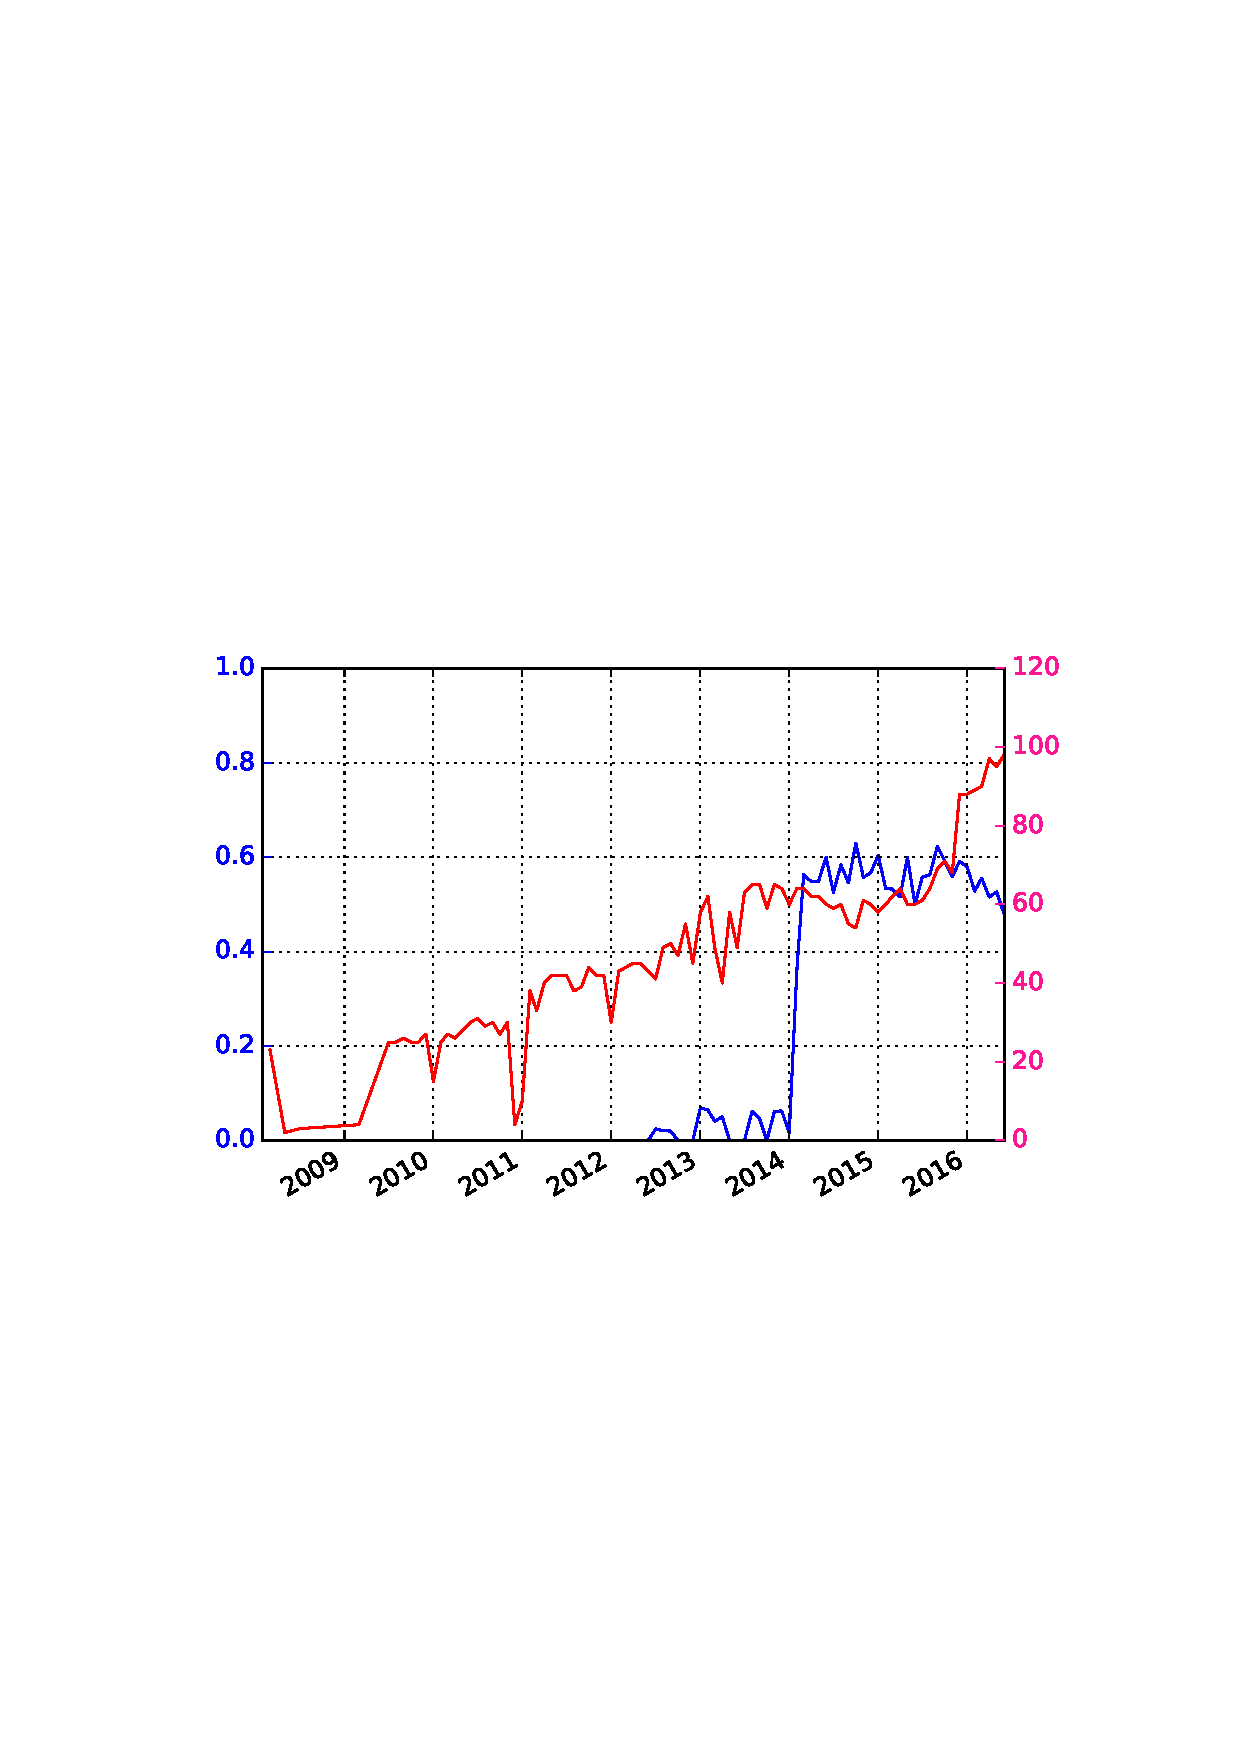
\includegraphics[width=\linewidth]{img/convergence_over_time_a.png}
			\caption{A-Root}
			\label{fig:convergence-a}			
		\end{subfigure}
		\begin{subfigure}{.32\textwidth}
			\centering
			\includegraphics[width=\linewidth]{img/convergence_over_time_c.png}
			\caption{C-Root}
			\label{fig:convergence-c}
		\end{subfigure}		
		\begin{subfigure}{.32\textwidth}
			\centering
			\includegraphics[width=\linewidth]{img/convergence_over_time_d.png}
			\caption{D-Root}
			\label{fig:convergence-d}
		\end{subfigure}		
		\begin{subfigure}{.32\textwidth}
			\centering
			\includegraphics[width=\linewidth]{img/convergence_over_time_f.png}
			\caption{F-Root}
			\label{fig:app:convergence-f}
		\end{subfigure}				
		\begin{subfigure}{.32\textwidth}
			\centering
			\includegraphics[width=\linewidth]{img/convergence_over_time_i.png}
			\caption{I-Root}
			\label{fig:convergence-i}
		\end{subfigure}								
		\begin{subfigure}{.32\textwidth}
			\centering
			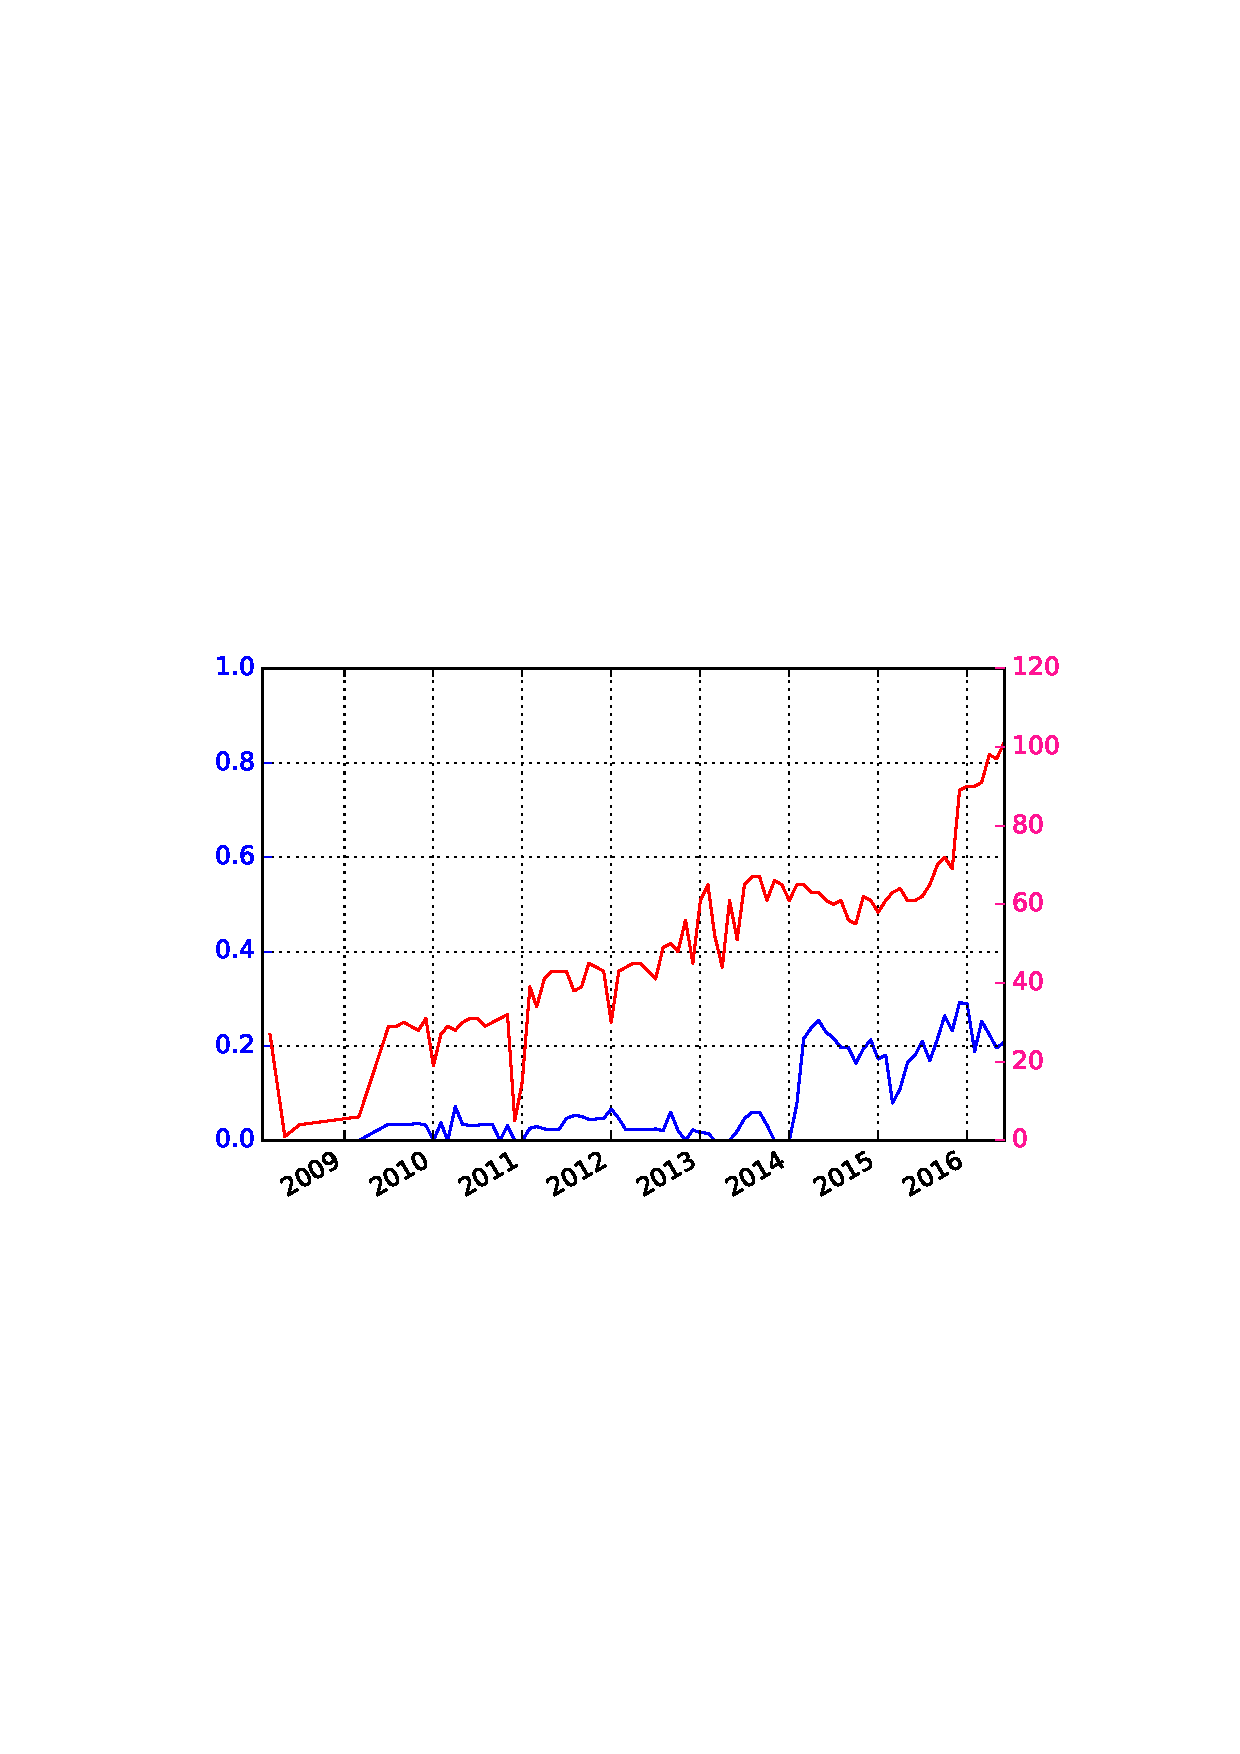
\includegraphics[width=\linewidth]{img/convergence_over_time_j.png}
			\caption{J-Root}
			\label{fig:convergence-j}
		\end{subfigure}										
		\begin{subfigure}{.32\textwidth}
			\centering
			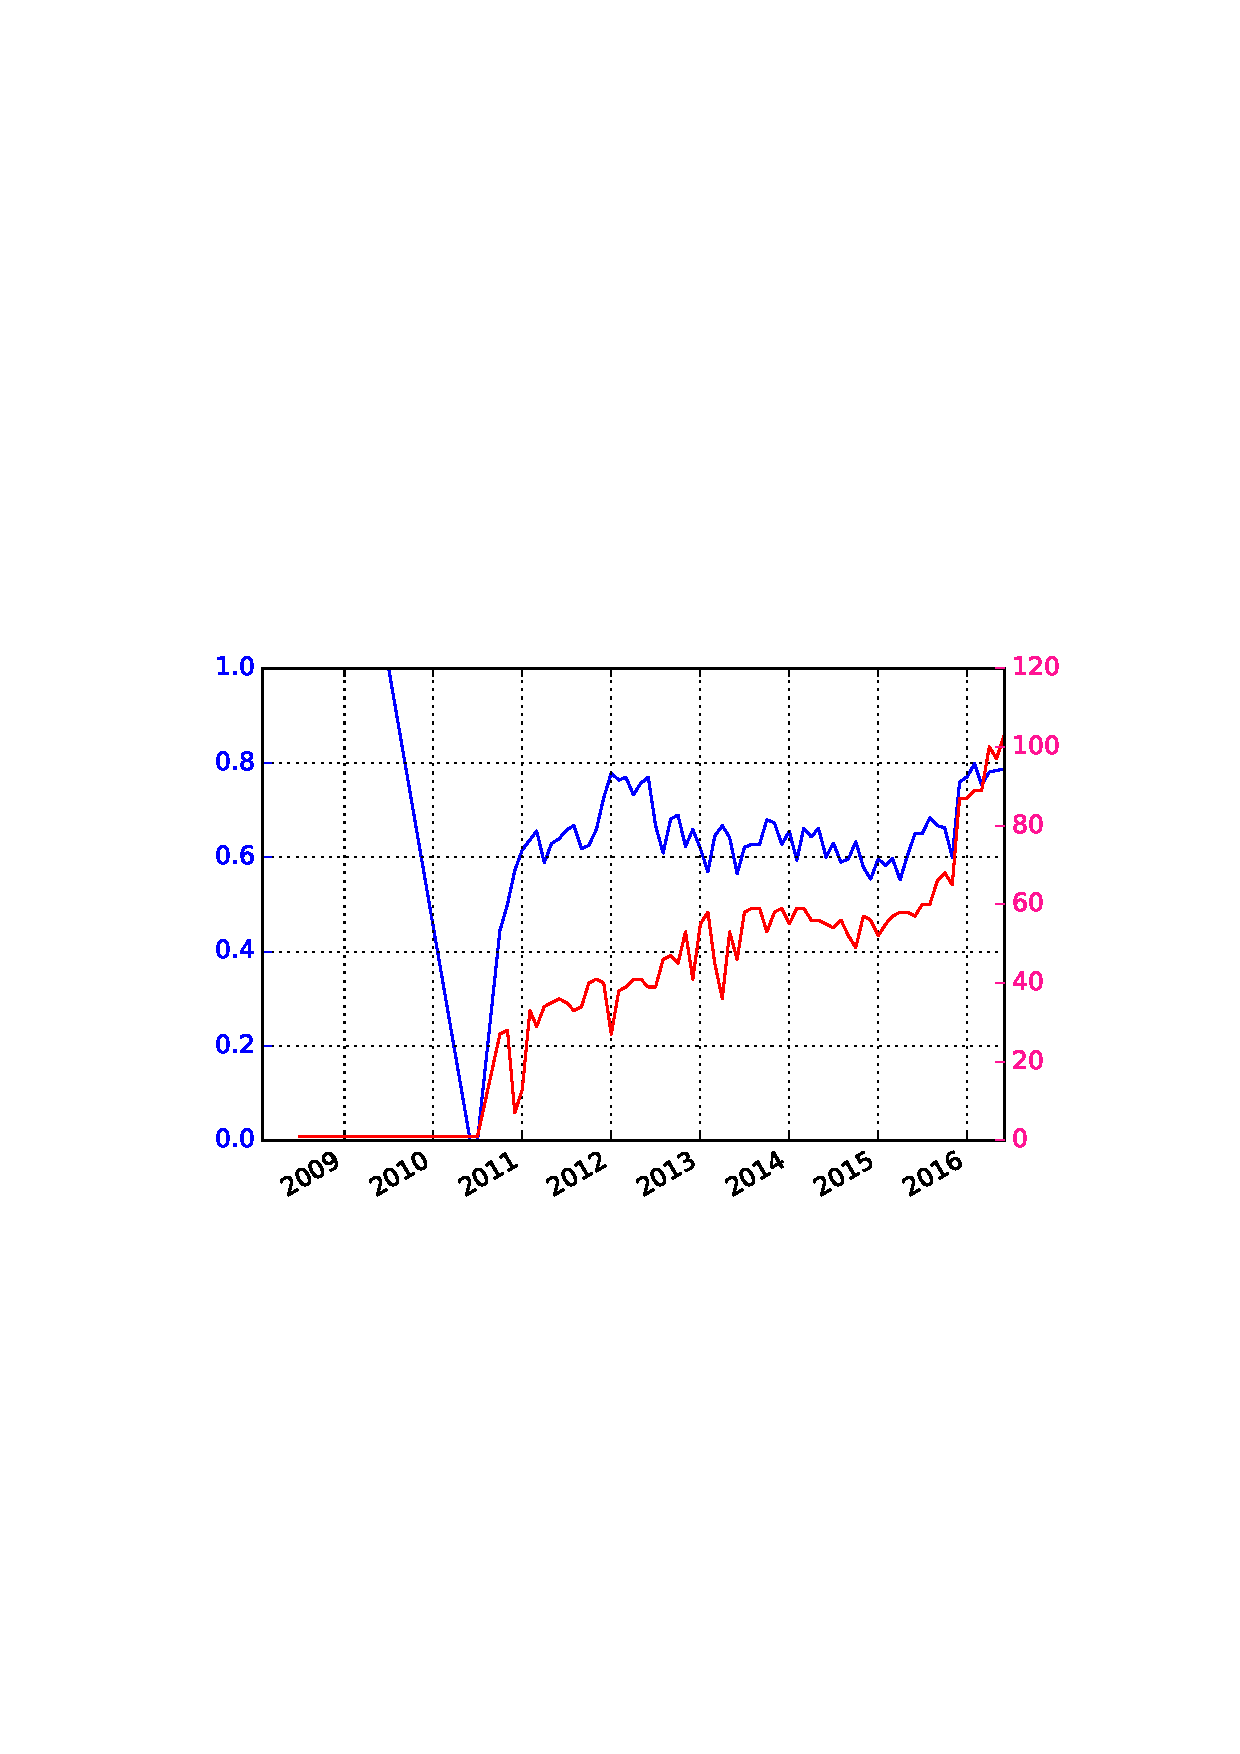
\includegraphics[width=\linewidth]{img/convergence_over_time_k.png}
			\caption{K-Root}
			\label{fig:convergence-k}
		\end{subfigure}											
		\begin{subfigure}{.32\textwidth}
			\centering
			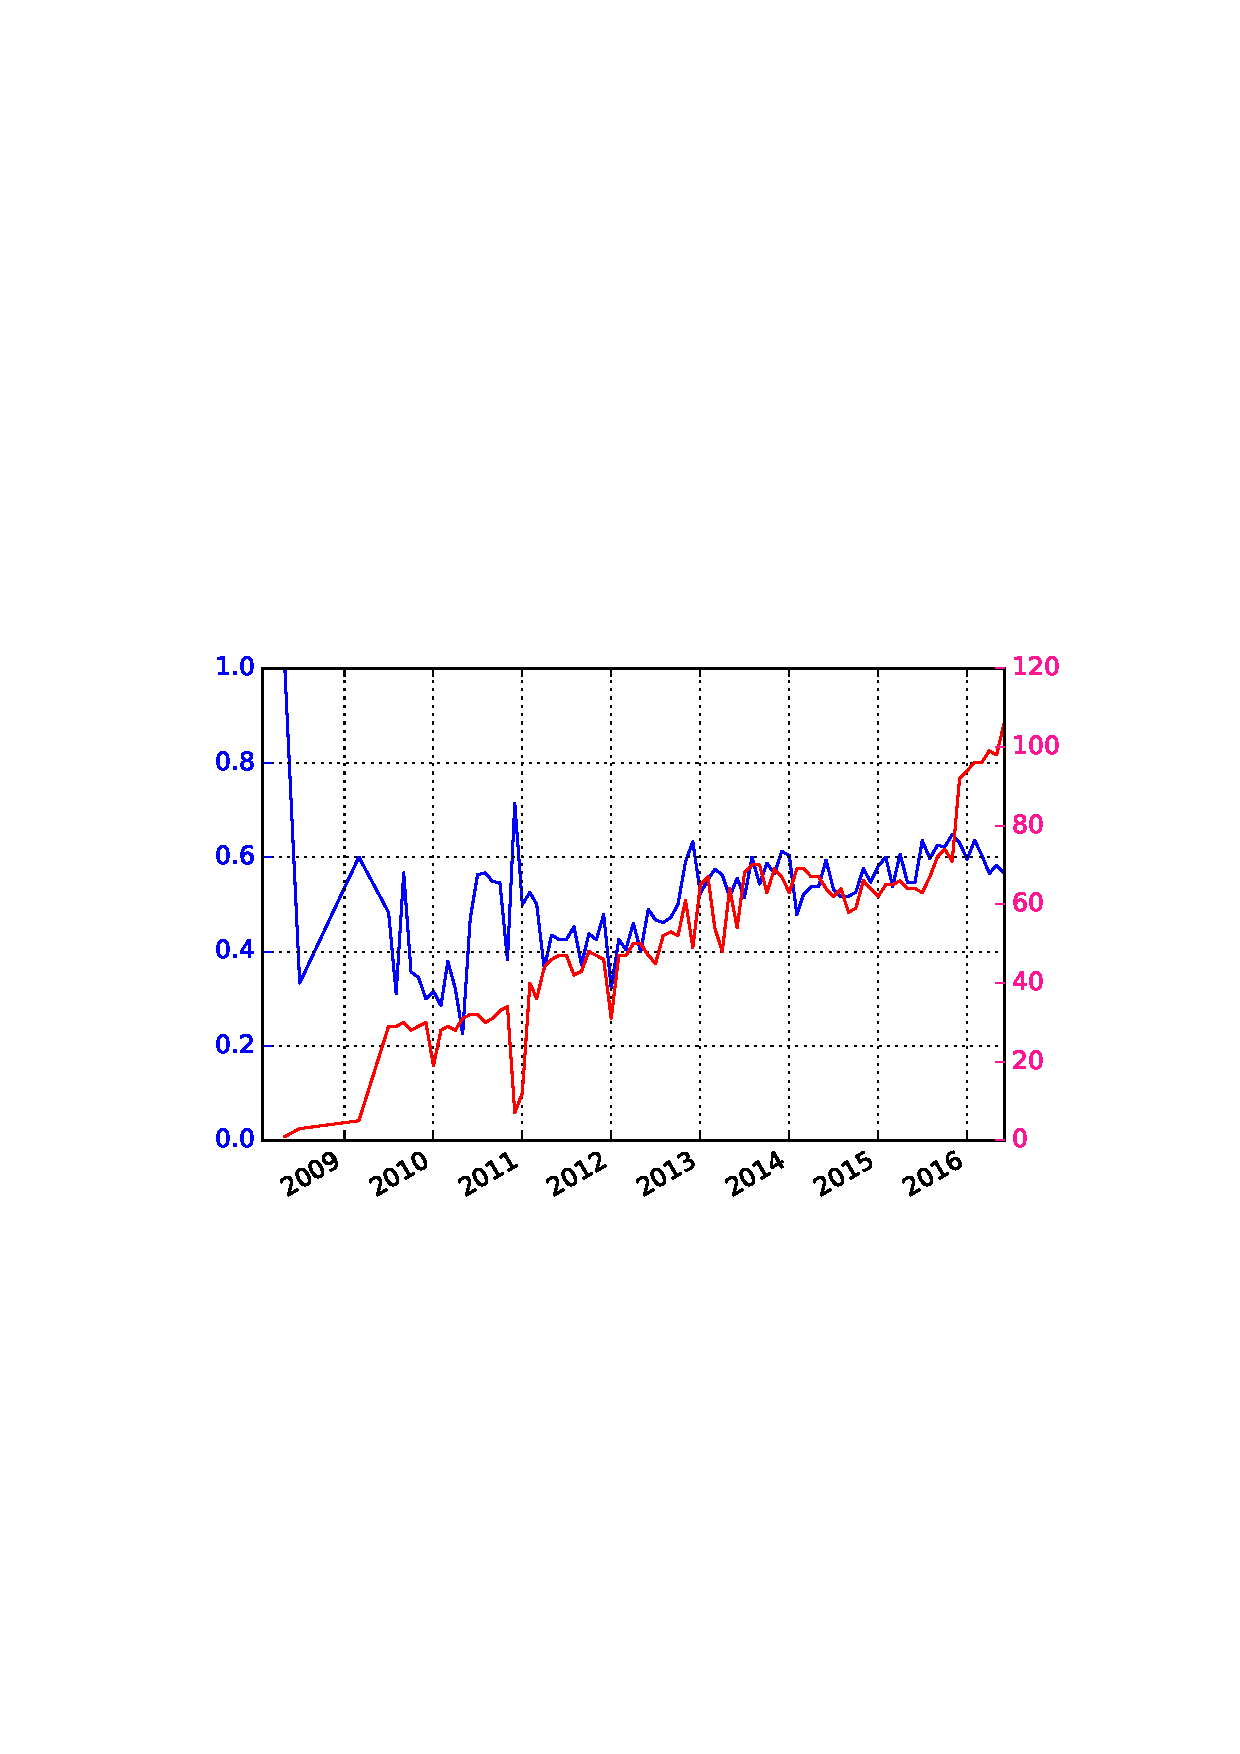
\includegraphics[width=\linewidth]{img/convergence_over_time_l.png}
			\caption{L-Root}
			\label{fig:convergence-l}
		\end{subfigure}											
		\begin{subfigure}{.32\textwidth}
			\centering
			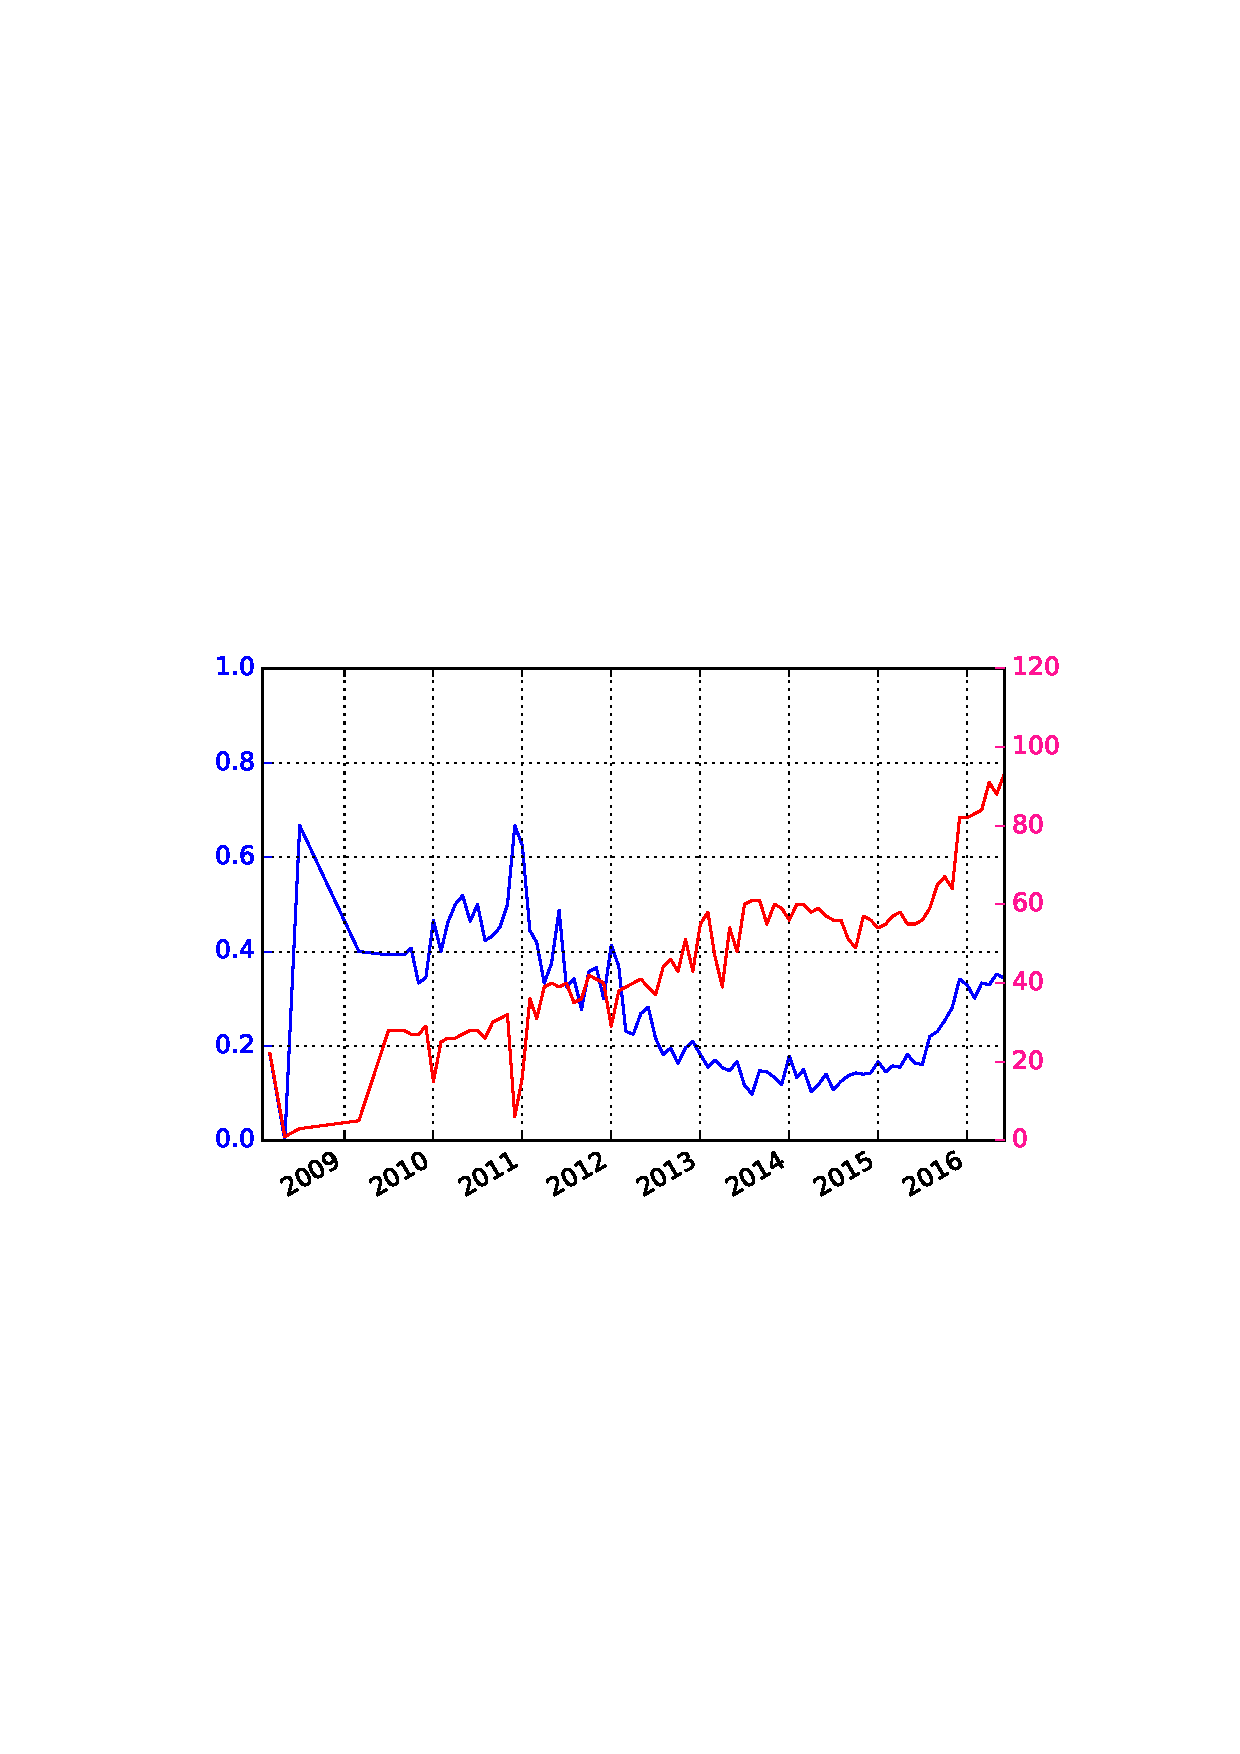
\includegraphics[width=\linewidth]{img/convergence_over_time_m.png}
			\caption{M-Root}
			\label{fig:app:convergence-m}
		\end{subfigure}
		\caption{Convergence level}
		\label{fig:app:convergence}	
	\end{figure}
	

	
	\chapter{VPs Composition}
	\label{app:peer-composition}
	A mutual VP can have either diverging or converging IPv4/IPv6 paths. For diverging paths, it can be: \textit{(i)} have shorter IPv4 path, \textit{(ii)} have shorter IPv6 path, or \textit{(iii)} have equal path length. The following graphs represent the VPs composition in terms of the aforementioned categorization for each Root Server. To provide better readability, the height of each stacked bar is normalized and the total number of VPs per time is displayed at the top of the graph.
	
	\begin{figure}[!htb]
		\centering
		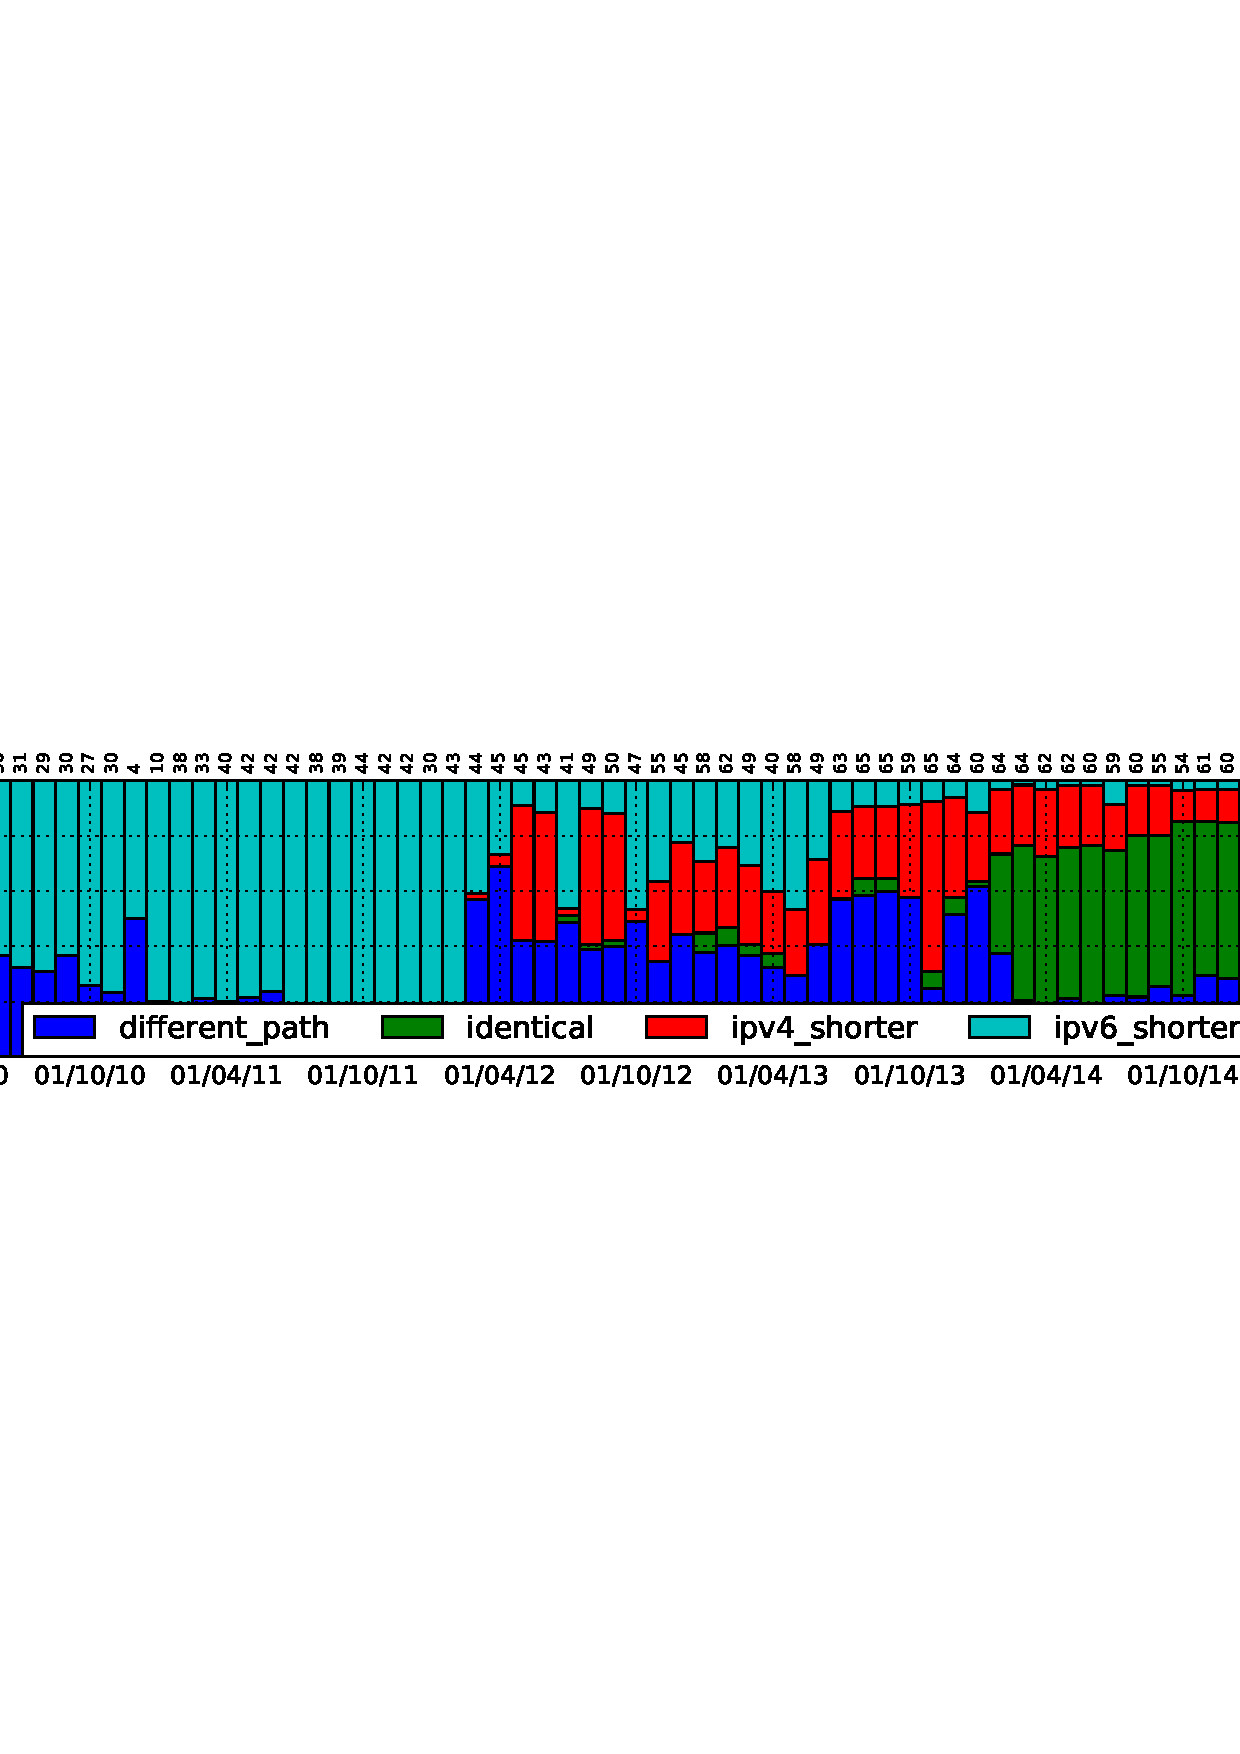
\includegraphics[width=6.0in]{img/peer_composition_a.png}
		\caption{A-Root peers composition}
		\label{fig:peer-comp-a}
	\end{figure}
	\begin{figure}[!htb]
		\centering
		\includegraphics[width=6.0in]{img/peer_composition_c.png}
		\caption{C-Root VPs composition}
		\label{fig:peer-comp-c}
	\end{figure}
	\begin{figure}[!htb]
		\centering
		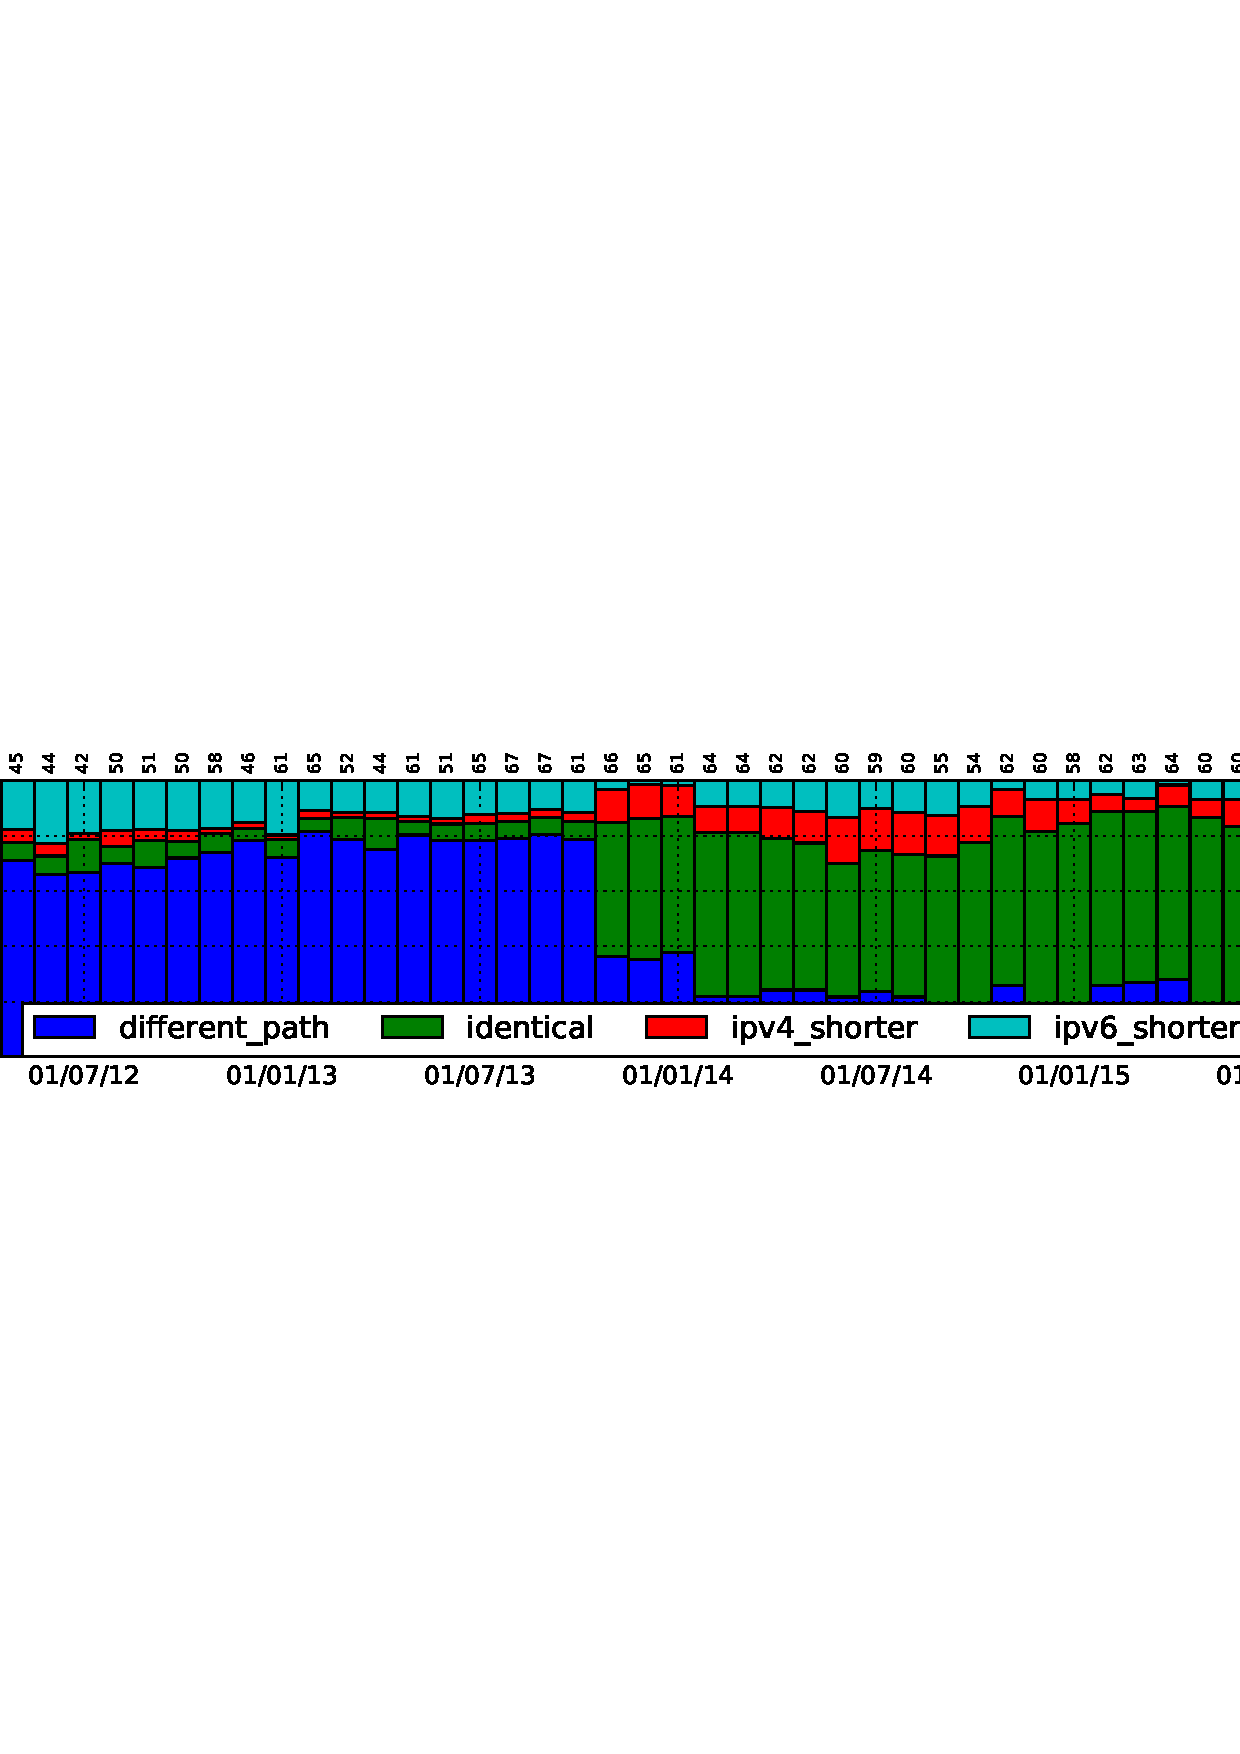
\includegraphics[width=6.0in]{img/peer_composition_d.png}
		\caption{D-Root VPs composition}
		\label{fig:peer-comp-d}
	\end{figure}
	\begin{figure}[!htb]
		\centering
		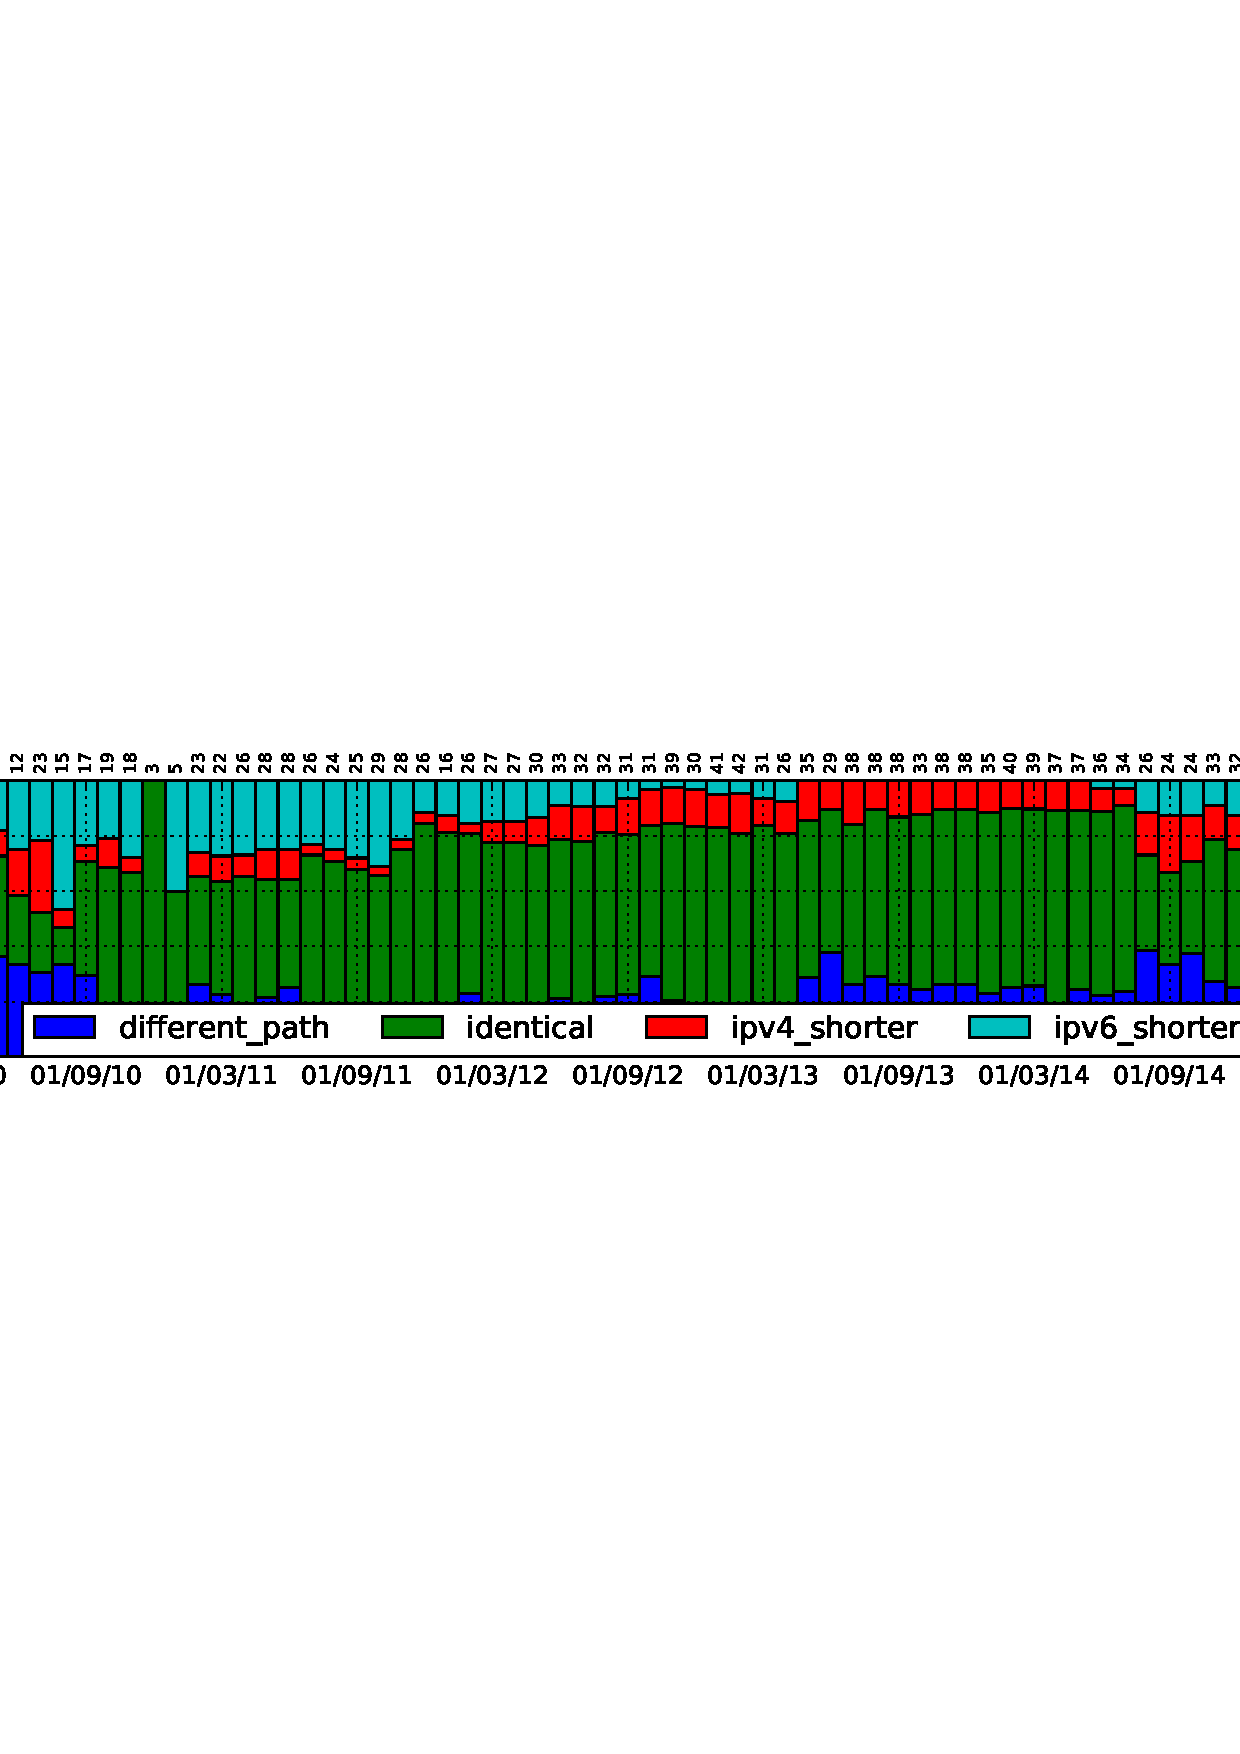
\includegraphics[width=6.0in]{img/peer_composition_f.png}
		\caption{F-Root VPs composition}
		\label{fig:peer-comp-f}
	\end{figure}
	\begin{figure}[!htb]
		\centering
		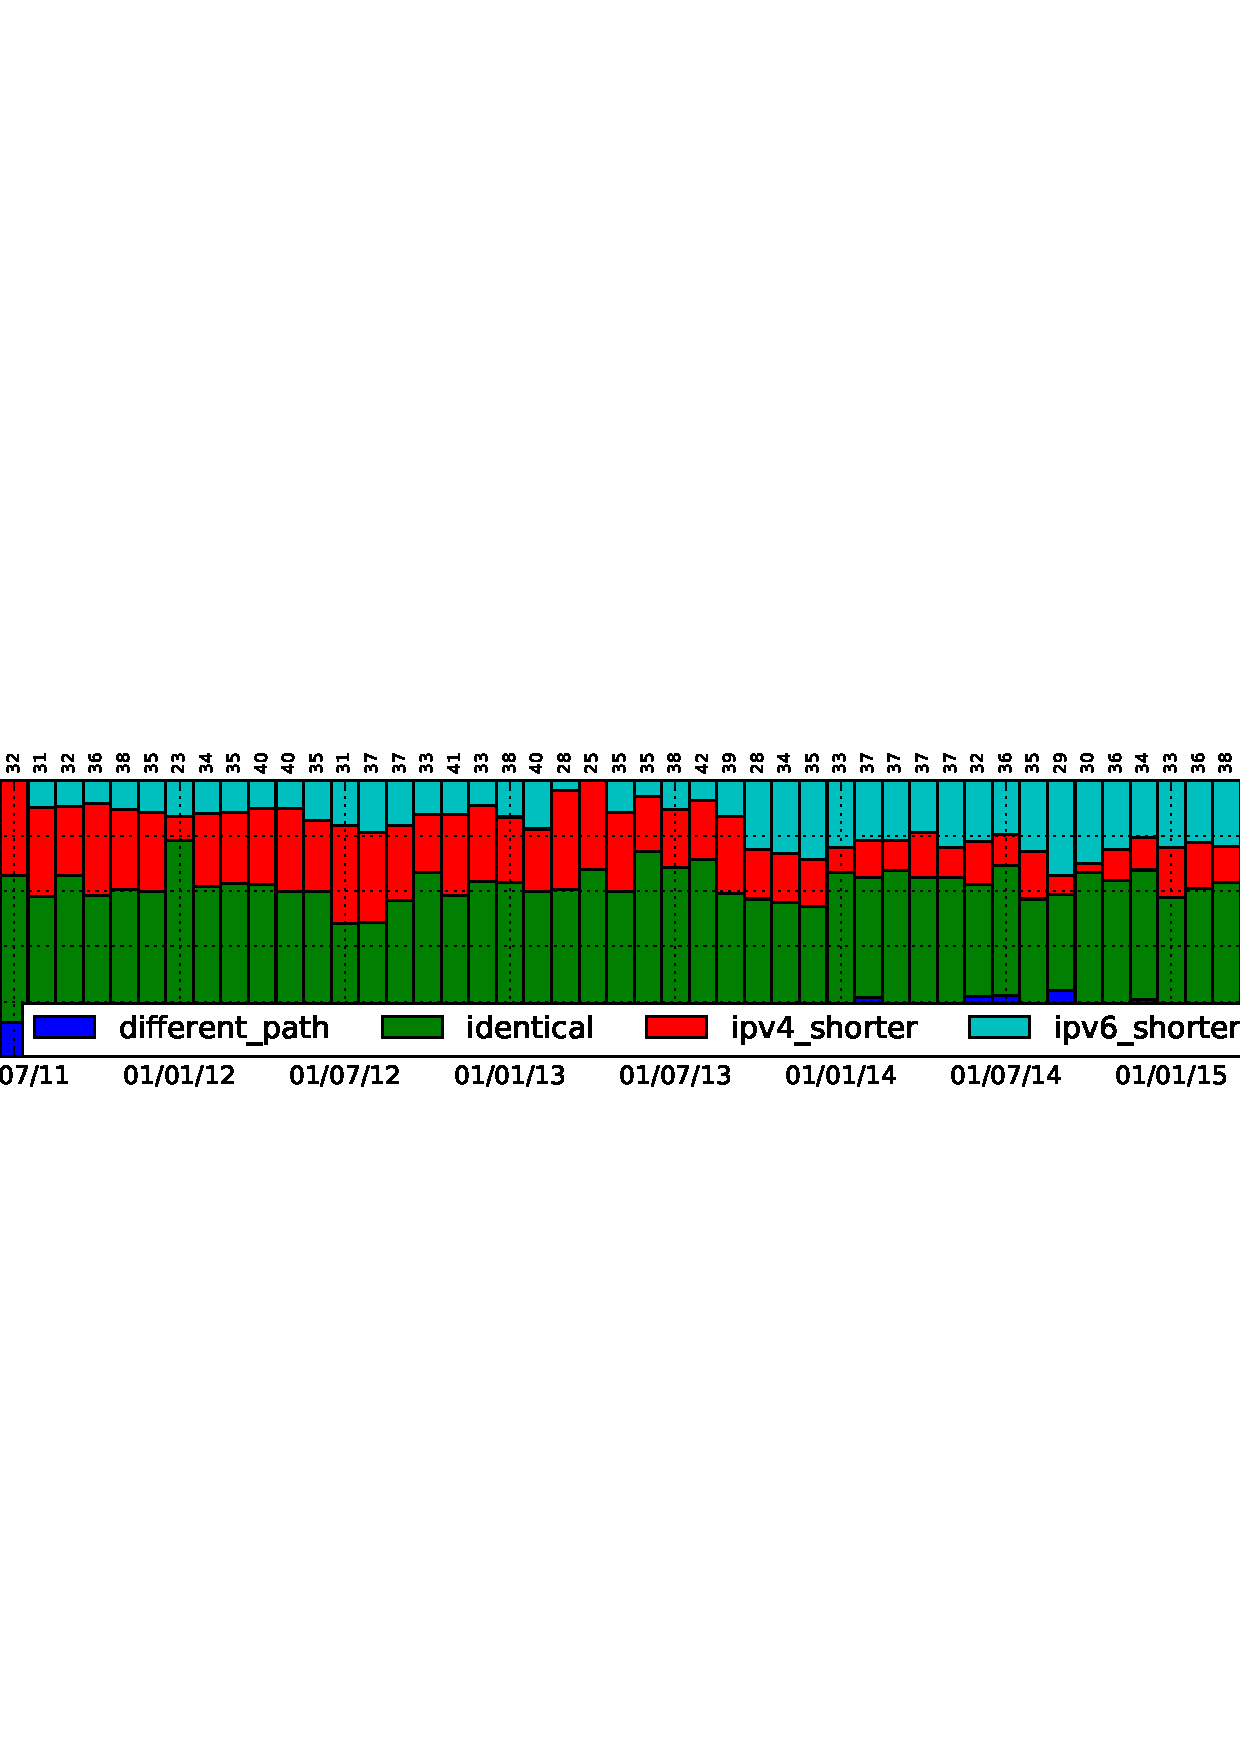
\includegraphics[width=6.0in]{img/peer_composition_i.png}
		\caption{I-Root VPs composition}
		\label{fig:peer-comp-i}
	\end{figure}
	\begin{figure}[!htb]
		\centering
		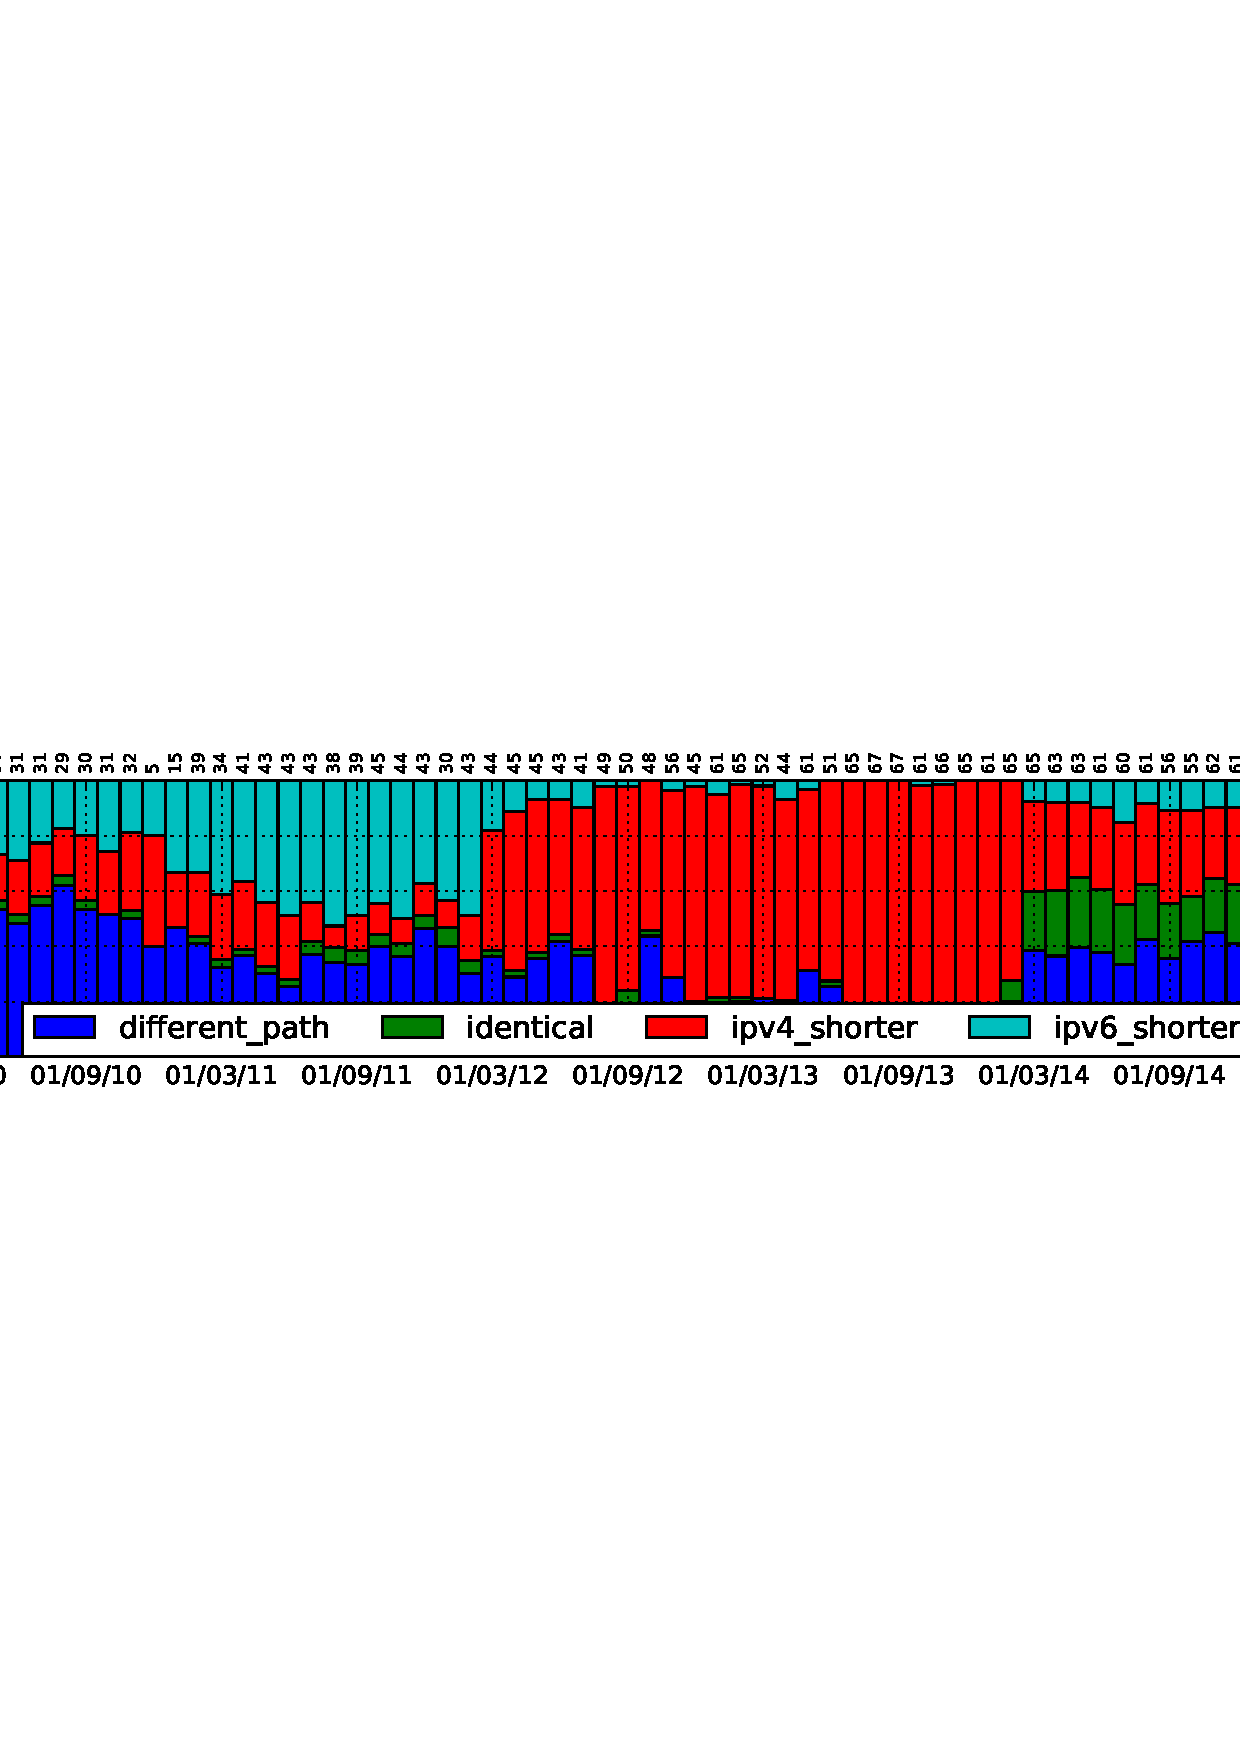
\includegraphics[width=6.0in]{img/peer_composition_j.png}
		\caption{J-Root VPs composition}
		\label{fig:peer-comp-j}
	\end{figure}
	\begin{figure}[!htb]
		\centering
		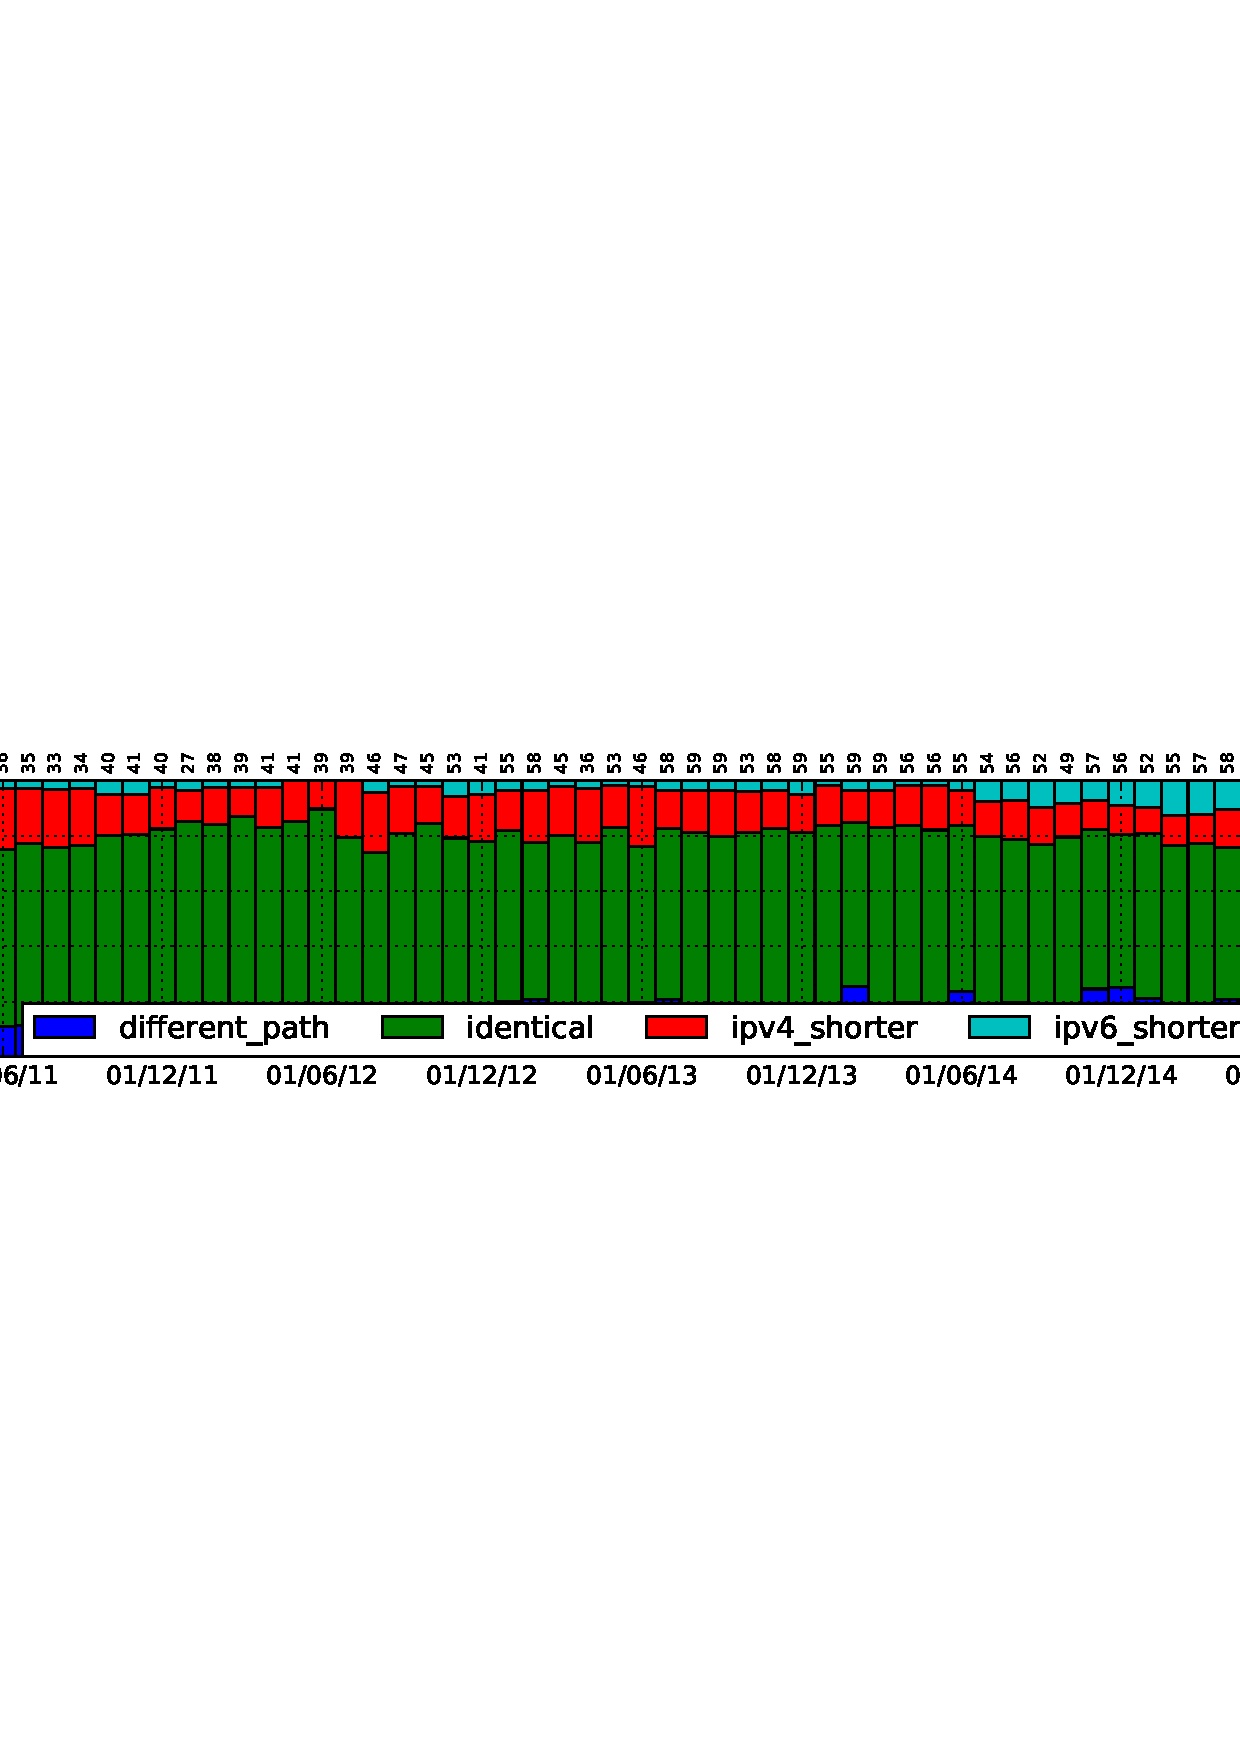
\includegraphics[width=6.0in]{img/peer_composition_k.png}
		\caption{K-Root VPs composition}
		\label{fig:peer-comp-k}
	\end{figure}
	\begin{figure}[!htb]
		\centering
		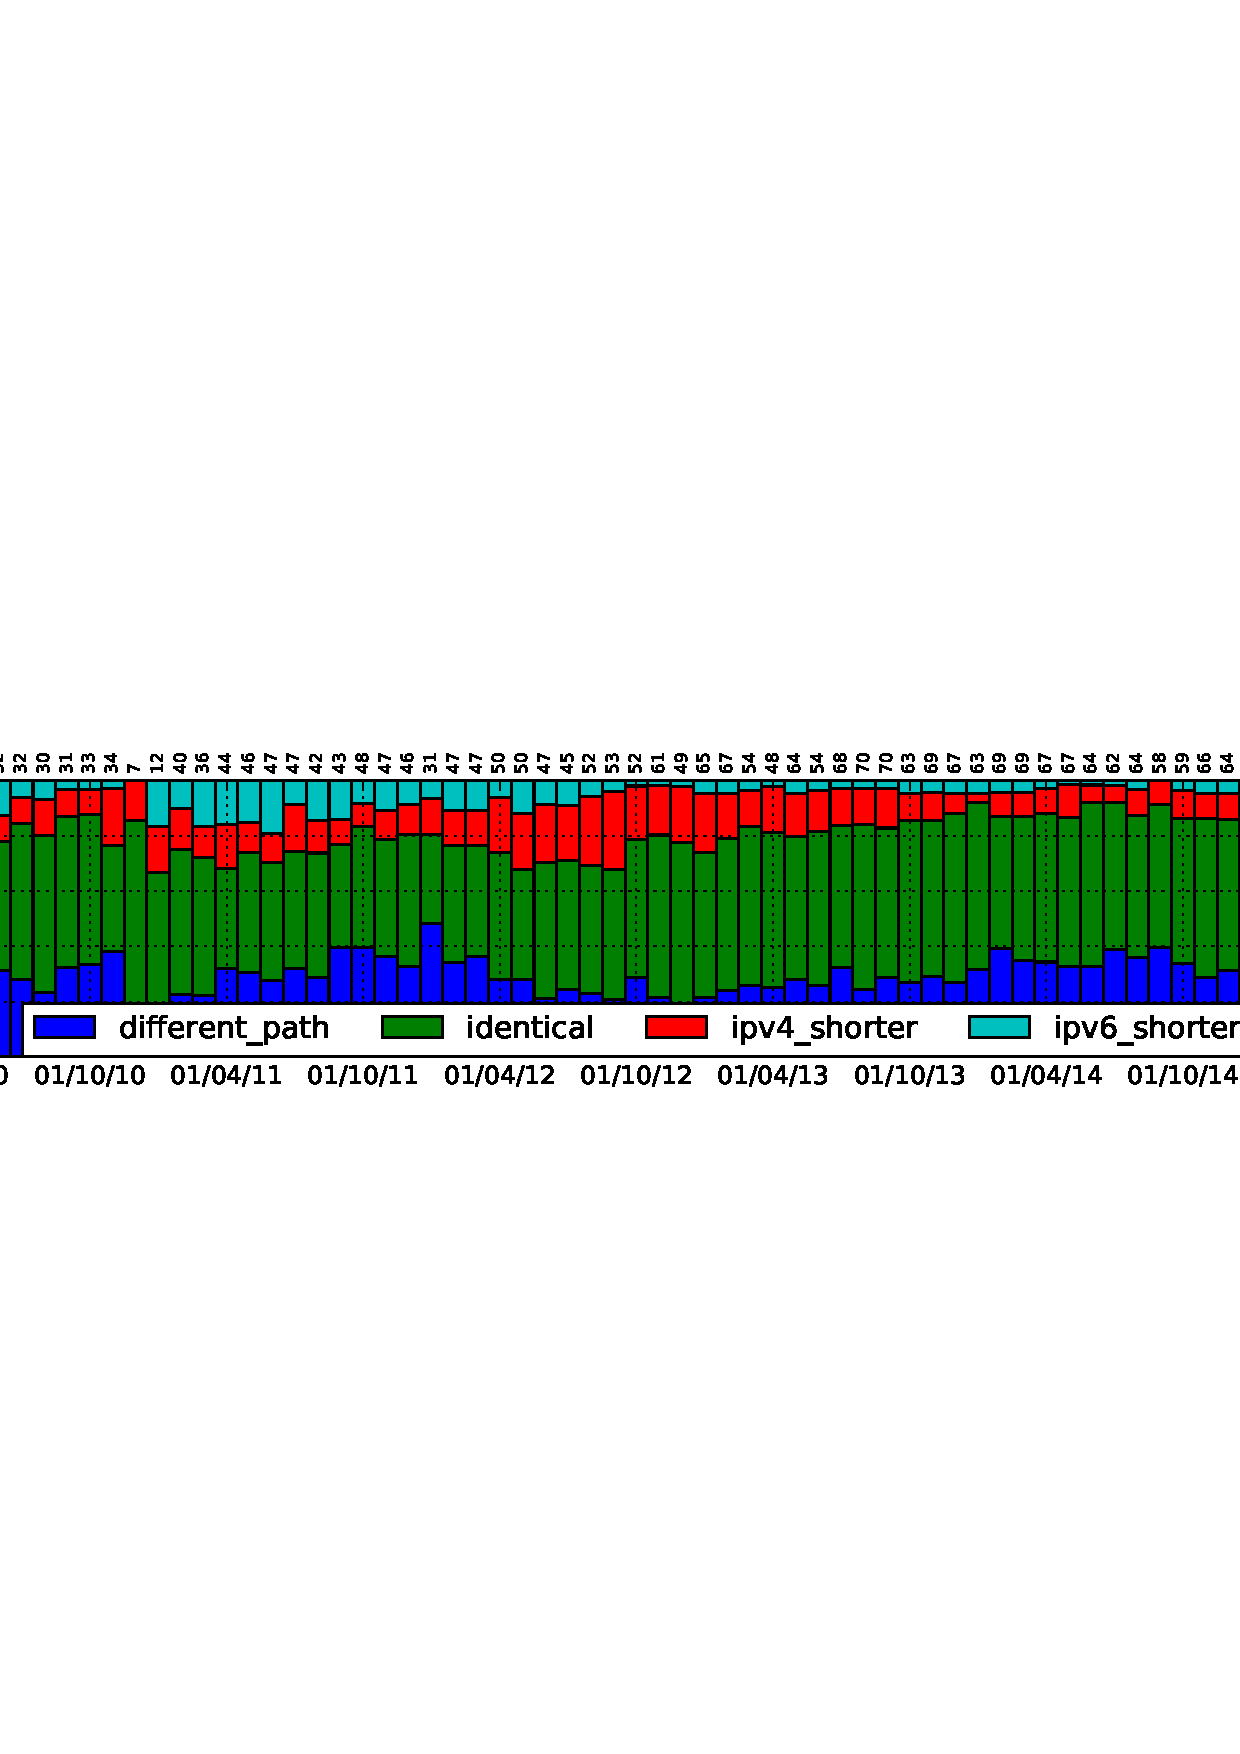
\includegraphics[width=6.0in]{img/peer_composition_l.png}
		\caption{L-Root VPs composition}
		\label{fig:peer-comp-l}
	\end{figure}
	\begin{figure}[!htb]
		\centering
		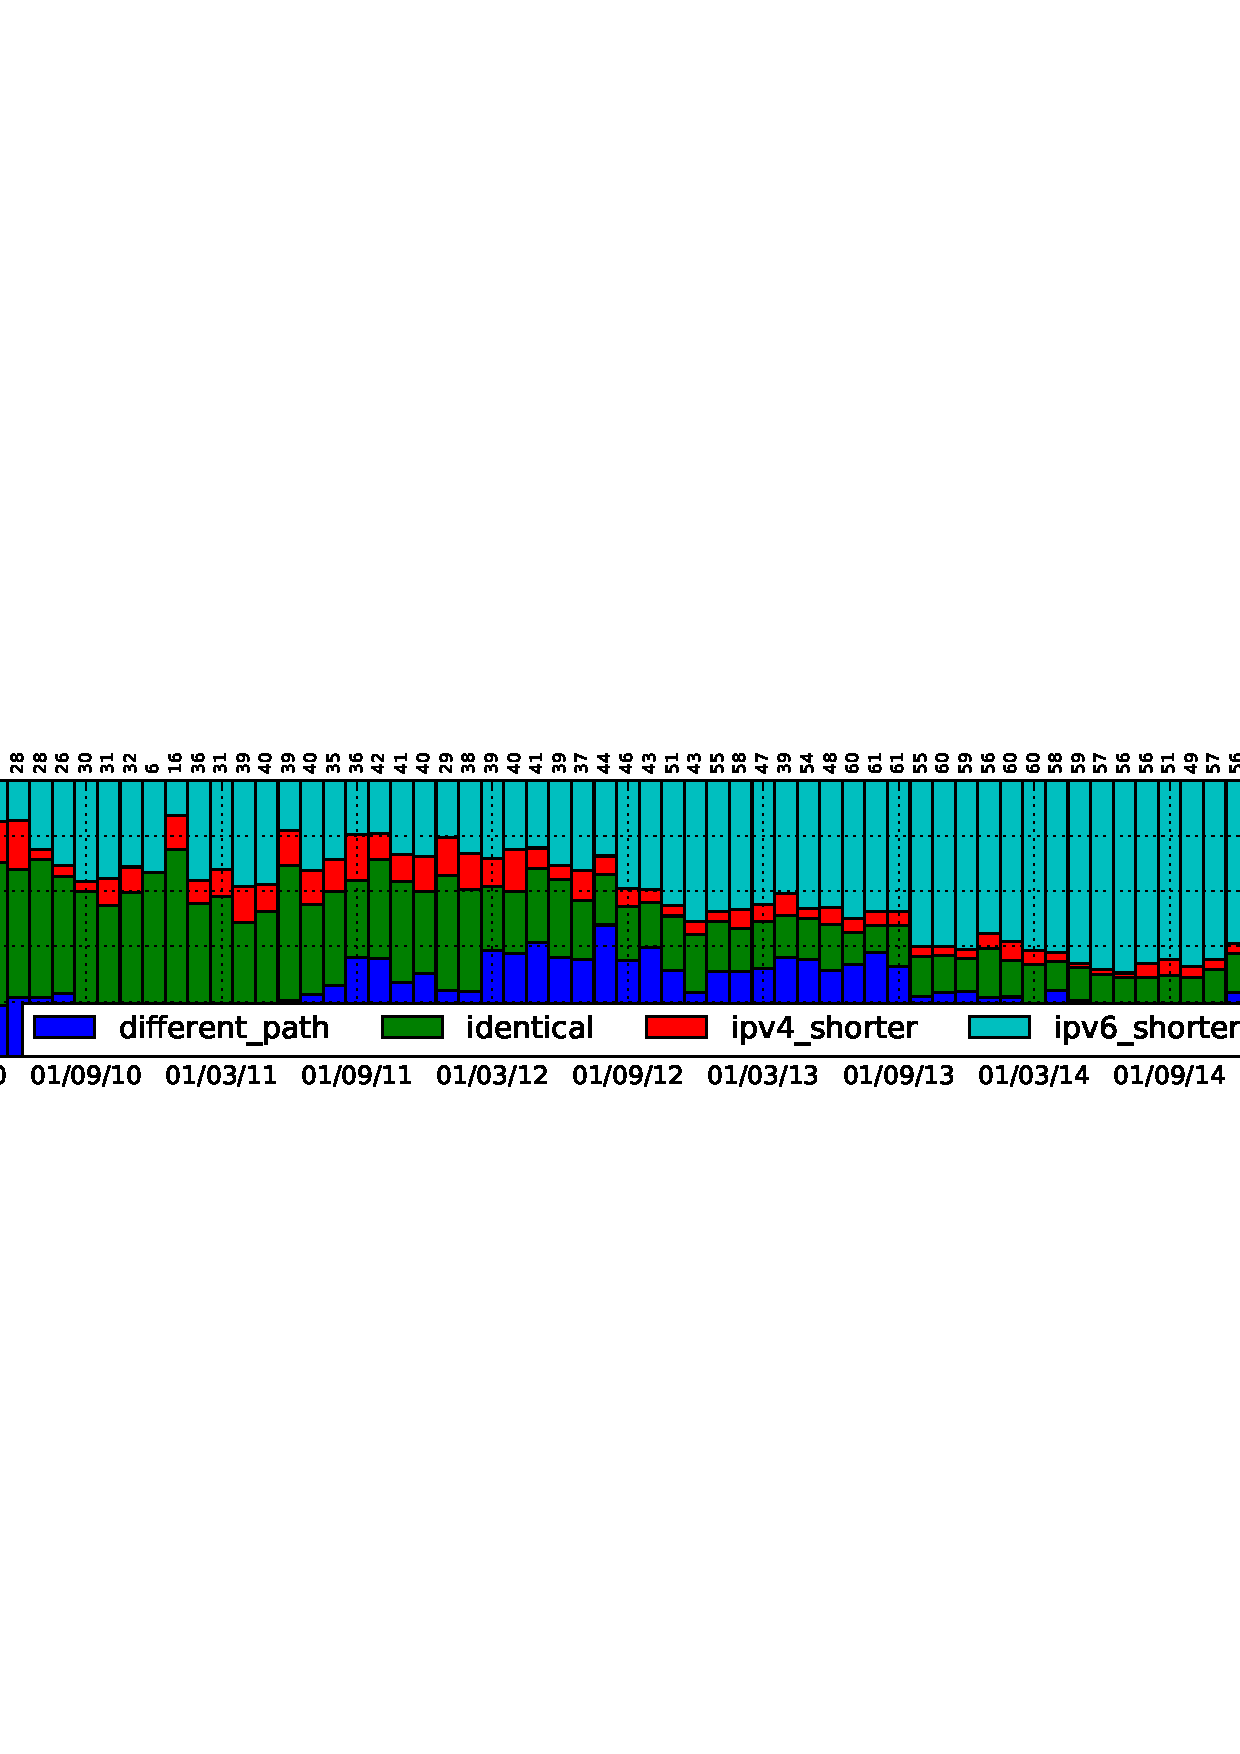
\includegraphics[width=6.0in]{img/peer_composition_m.png}
		\caption{M-Root VPs composition}
		\label{fig:peer-comp-m}
	\end{figure}
	
	\chapter{AS Path Length Distribution}
	\label{app:path-avg}
	
	The box plot is generated using Matplotlib with default configuration. The closed box comprising of three horizontally parallel lines represents the 1\textsuperscript{st} quartile, the median, and the 3\textsuperscript{rd} quartile (bottom to top). Interquartile range (IQR) is defined as the range between 1\textsuperscript{st} quartile and 3\textsuperscript{rd} quartile. The top whisker represents the maximum value below 75\% + 1.5 IQR, while the bottom one represents the minimum value above 25\% - 1.5 IQR. Any value falls outside those boundaries are regarded as outlier (plotted as '+'). The green line represents the median of all path length values over the time.
	
	Appendix \ref{app:path-avg:all-peers} represents AS path length distribution for all mutual VPs, regardless diverging or converging. Appendix \ref{app:path-avg:diff-paths} represents the distribution only for diverging VPs.
	\section{All VPs}
	\label{app:path-avg:all-peers}
		\begin{figure}[!htb]
			\centering
			\includegraphics[width=6.0in]{img/path_avg_all_a.png}
			\caption{Path average length of all peers of A-Root}
			\label{fig:path-avg-all-a}
		\end{figure}
		\begin{figure}[!htb]
			\centering
			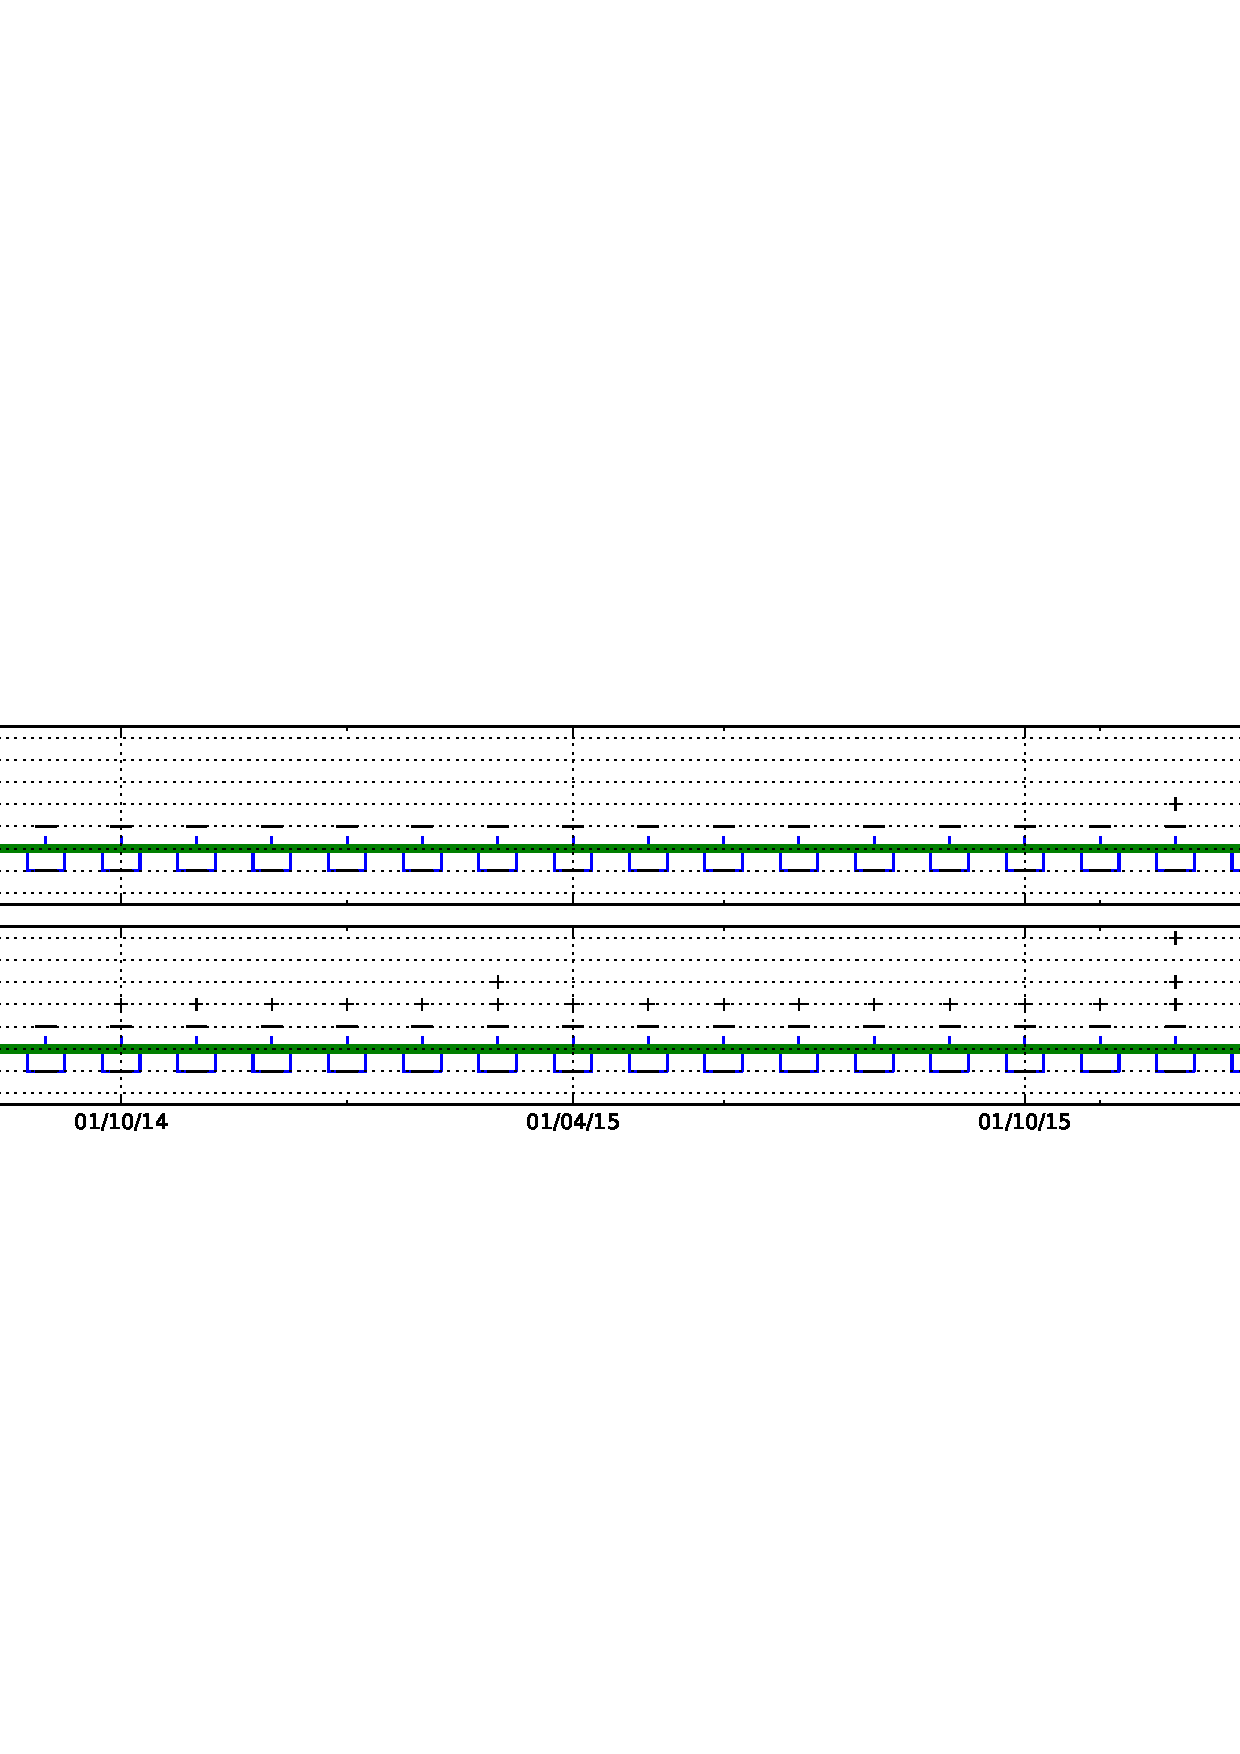
\includegraphics[width=6.0in]{img/path_avg_all_c.png}
			\caption{Path length distribution of all C-Root's VPs}
			\label{fig:path-avg-all-c}
		\end{figure}
		\begin{figure}[!htb]
			\centering
			\includegraphics[width=6.0in]{img/path_avg_all_d.png}
			\caption{Path length distribution of all D-Root's VPs}
			\label{fig:path-avg-all-d}
		\end{figure}
		\begin{figure}[!htb]
			\centering
			\includegraphics[width=6.0in]{img/path_avg_all_f.png}
			\caption{Path length distribution of all F-Root's VPs}
			\label{fig:path-avg-all-f}
		\end{figure}
		
		\begin{figure}[!htb]
			\centering
			\includegraphics[width=6.0in]{img/path_avg_all_i.png}
			\caption{Path length distribution of all I-Root's VPs}
			\label{fig:path-avg-all-i}
		\end{figure}
		
		\begin{figure}[!htb]
			\centering
			\includegraphics[width=6.0in]{img/path_avg_all_j.png}
			\caption{Path length distribution of all J-Root's VPs}
			\label{fig:path-avg-all-j}
		\end{figure}
		\begin{figure}[!htb]
			\centering
			\includegraphics[width=6.0in]{img/path_avg_all_k.png}
			\caption{Path length distribution of all K-Root's VPs}
			\label{fig:path-avg-all-k}
		\end{figure}
		\begin{figure}[!htb]
			\centering
			\includegraphics[width=6.0in]{img/path_avg_all_l.png}
			\caption{Path length distribution of all L-Root's VPs}
			\label{fig:path-avg-all-l}
		\end{figure}
		\begin{figure}[htbp]
			\centering
			\includegraphics[width=6.0in]{img/path_avg_all_m.png}
			\caption{Path length distribution of all M-Root's VPs}
			\label{fig:path-avg-all-m}
		\end{figure}

	\clearpage		
	\section{Only for VPs with Diverging IPv4/IPv6 Paths}
	\label{app:path-avg:diff-paths}
		\begin{figure}[!htb]
			\centering
			\includegraphics[width=6.0in]{img/path_avg_diff_a.png}
			\caption{Average path length of A-Root peers that have different IPv4/IPv6 paths}
			\label{fig:path-avg-diff-a}
		\end{figure}
		\begin{figure}[!htb]
			\centering
			\includegraphics[width=6.0in]{img/path_avg_diff_c.png}
			\caption{Average path length of C-Root peers that have different IPv4/IPv6 paths}
			\label{fig:path-avg-diff-c}
		\end{figure}
		\begin{figure}[!htb]
			\centering
			\includegraphics[width=6.0in]{img/path_avg_diff_d.png}
			\caption{Average path length of D-Root peers that have different IPv4/IPv6 paths}
			\label{fig:path-avg-diff-d}
		\end{figure}
		\begin{figure}[!htb]
			\centering
			\includegraphics[width=6.0in]{img/path_avg_diff_f.png}
			\caption{Average path length of F-Root peers that have different IPv4/IPv6 paths}
			\label{fig:path-avg-diff-f}
		\end{figure}
		\begin{figure}[!htb]
			\centering
			\includegraphics[width=6.0in]{img/path_avg_diff_i.png}
			\caption{Average path length of I-Root peers that have different IPv4/IPv6 paths}
			\label{fig:path-avg-diff-i}
		\end{figure}
		\begin{figure}[!htb]
			\centering
			\includegraphics[width=6.0in]{img/path_avg_diff_j.png}
			\caption{Average path length of J-Root peers that have different IPv4/IPv6 paths}
			\label{fig:path-avg-diff-j}
		\end{figure}
		\begin{figure}[!htb]
			\centering
			\includegraphics[width=6.0in]{img/path_avg_diff_k.png}
			\caption{Average path length of K-Root peers that have different IPv4/IPv6 paths}
			\label{fig:path-avg-diff-k}
		\end{figure}
		\begin{figure}[!htb]
			\centering
			\includegraphics[width=6.0in]{img/path_avg_diff_l.png}
			\caption{Average path length of L-Root peers that have different IPv4/IPv6 paths}
			\label{fig:path-avg-diff-l}
		\end{figure}
		\begin{figure}[!htb]
			\centering
			\includegraphics[width=6.0in]{img/path_avg_diff_m.png}
			\caption{Average path length of M-Root peers that have different IPv4/IPv6 paths}
			\label{fig:path-avg-diff-m}
		\end{figure}	
	
	\chapter{VP Length Degree}
	\label{app:peer-degree-dist}
	The Root Server's diverging VPs 
	
	\begin{figure}[!htb]
		\centering
		\includegraphics[width=6.5in]{img/peer_degree_diff_a.png}
		\caption{VP degree distribution of A-Root}
		\label{fig:app:peer-deg-dist-diff-a}
	\end{figure}
	\begin{figure}[!htb]
		\centering
		\includegraphics[width=6.5in]{img/peer_degree_diff_c.png}
		\caption{VP degree distribution of C-Root}
		\label{fig:app:peer-deg-dist-diff-c}
	\end{figure}
	\begin{figure}[!htb]
		\centering
		\includegraphics[width=6.5in]{img/peer_degree_diff_d.png}
		\caption{VP degree distribution of D-Root}
		\label{fig:app:peer-deg-dist-diff-d}
	\end{figure}
	\begin{figure}
		\centering
		\includegraphics[width=6.5in]{img/peer_degree_diff_f.png}
		\caption{VP degree distribution of F-Root}
		\label{fig:app:peer-deg-dist-diff-f}
	\end{figure}
	\begin{figure}
		\centering
		\includegraphics[width=6.5in]{img/peer_degree_diff_i.png}
		\caption{VP degree distribution of I-Root}
		\label{fig:app:peer-deg-dist-diff-i}
	\end{figure}
	\begin{figure}
		\centering
		\includegraphics[width=6.5in]{img/peer_degree_diff_j.png}
		\caption{VP degree distribution of J-Root}
		\label{fig:app:peer-deg-dist-diff-j}
	\end{figure}
	\begin{figure}
		\centering
		\includegraphics[width=6.5in]{img/peer_degree_diff_k.png}
		\caption{VP degree distribution of K-Root}
		\label{fig:app:peer-deg-dist-diff-k}
	\end{figure}
	\begin{figure}
		\centering
		\includegraphics[width=6.5in]{img/peer_degree_diff_l.png}
		\caption{VP degree distribution of L-Root}
		\label{fig:app:peer-deg-dist-diff-l}
	\end{figure}
	\begin{figure}[!htb]
		\centering
		\includegraphics[width=6.5in]{img/peer_degree_diff_m.png}
		\caption{VP degree distribution of M-Root}
		\label{fig:app:peer-deg-dist-diff-m}
	\end{figure}
	
	
	\chapter{Average Path Length Differences for VPs with Shorter IPv4 Path}
	\label{app:shorter-ipv4}
	\begin{figure}[!htb]
		\centering
		\includegraphics[width=6.0in]{img/shorter-ipv4-a.png}
		\caption{Path length differences for A-Root's VPs with shorter IPv4 path}
		\label{fig:shorter-ipv4-a}
	\end{figure}
	\begin{figure}[!htb]
		\centering
		\includegraphics[width=6.0in]{img/shorter-ipv4-c.png}
		\caption{Path length differences for C-Root's VPs with shorter IPv4 path}
		\label{fig:shorter-ipv4-c}
	\end{figure}
	\begin{figure}[!htb]
		\centering
		\includegraphics[width=6.0in]{img/shorter-ipv4-d.png}
		\caption{Path length differences for D-Root's VPs with shorter IPv4 path}
		\label{fig:shorter-ipv4-d}
	\end{figure}
	\begin{figure}[!htb]
		\centering
		\includegraphics[width=6.0in]{img/shorter-ipv4-f.png}
		\caption{Path length differences for F-Root's VPs with shorter IPv4 path}
		\label{fig:shorter-ipv4-f}
	\end{figure}
	\begin{figure}[!htb]
		\centering
		\includegraphics[width=6.0in]{img/shorter-ipv4-i.png}
		\caption{Path length differences for I-Root's VPs with shorter IPv4 path}
		\label{fig:shorter-ipv4-i}
	\end{figure}
	\begin{figure}[!htb]
		\centering
		\includegraphics[width=6.0in]{img/shorter-ipv4-j.png}
		\caption{Path length differences for J-Root's VPs with shorter IPv4 path}
		\label{fig:shorter-ipv4-j}
	\end{figure}
	\begin{figure}[!htb]
		\centering
		\includegraphics[width=6.0in]{img/shorter-ipv4-k.png}
		\caption{Path length differences for K-Root's VPs with shorter IPv4 path}
		\label{fig:shorter-ipv4-k}
	\end{figure}
	\begin{figure}[!htb]
		\centering
		\includegraphics[width=6.0in]{img/shorter-ipv4-l.png}
		\caption{Path length differences for L-Root's VPs with shorter IPv4 path}
		\label{fig:shorter-ipv4-l}
	\end{figure}
	\begin{figure}[!htb]
		\centering
		\includegraphics[width=6.0in]{img/shorter-ipv4-m.png}
		\caption{Path length differences for M-Root's VPs with shorter IPv4 path}
		\label{fig:shorter-ipv4-m}
	\end{figure}
	
	\chapter{Average Path Length Differences for VPs with Shorter IPv6 Path}
	\label{app:shorter-ipv6}
	\begin{figure}[!htb]
		\centering
		\includegraphics[width=6.0in]{img/shorter-ipv6-a.png}
		\caption{Path length differences for A-Root's VPs with shorter IPv6 path}
		\label{fig:app:shorter-ipv6-a}
	\end{figure}
	\begin{figure}[!htb]
		\centering
		\includegraphics[width=6.0in]{img/shorter-ipv6-c.png}
		\caption{Path length differences for C-Root's VPs with shorter IPv6 path}
		\label{fig:app:shorter-ipv6-c}
	\end{figure}
	\begin{figure}[!htb]
		\centering
		\includegraphics[width=6.0in]{img/shorter-ipv6-d.png}
		\caption{Path length differences for D-Root's VPs with shorter IPv6 path}
		\label{fig:app:shorter-ipv6-d}
	\end{figure}
	\begin{figure}[!htb]
		\centering
		\includegraphics[width=6.0in]{img/shorter-ipv6-f.png}
		\caption{Path length differences for F-Root's VPs with shorter IPv6 path}
		\label{fig:app:shorter-ipv6-f}
	\end{figure}
	\begin{figure}[!htb]
		\centering
		\includegraphics[width=6.0in]{img/shorter-ipv6-i.png}
		\caption{Path length differences for I-Root's VPs with shorter IPv6 path}
		\label{fig:app:shorter-ipv6-i}
	\end{figure}
	\begin{figure}[!htb]
		\centering
		\includegraphics[width=6.0in]{img/shorter-ipv6-j.png}
		\caption{Path length differences for J-Root's VPs with shorter IPv6 path}
		\label{fig:app:shorter-ipv6-j}
	\end{figure}
	\begin{figure}[!htb]
		\centering
		\includegraphics[width=6.0in]{img/shorter-ipv6-k.png}
		\caption{Path length differences for K-Root's VPs with shorter IPv6 path}
		\label{fig:app:shorter-ipv6-k}
	\end{figure}
	\begin{figure}[!htb]
		\centering
		\includegraphics[width=6.0in]{img/shorter-ipv6-l.png}
		\caption{Path length differences for L-Root's VPs with shorter IPv6 path}
		\label{fig:app:shorter-ipv6-l}
	\end{figure}
	\begin{figure}[!htb]
		\centering
		\includegraphics[width=6.0in]{img/shorter-ipv6-m.png}
		\caption{Path length differences for M-Root's VPs with shorter IPv6 path}
		\label{fig:app:shorter-ipv6-m}
	\end{figure}

\iffalse	
	\chapter{Physical Location}
	\label{app:physical-loc}
	\begin{figure}[!htb]
		\centering
		\includegraphics[width=6.0in]{img/coll-ams-ix.png}
		\caption{Peers with different IPv4/IPv6 paths detected by RIS Collector in AMS-IX and NL-IX, Amsterdam}
		\label{fig:coll-ams-ix}
	\end{figure}
	\begin{figure}[!htb]
		\centering
		\includegraphics[width=6.0in]{img/coll-barcelona.png}
		\caption{Peers with different IPv4/IPv6 paths detected by RIS Collector in CATNIX, Barcelona}
		\label{fig:coll-barcelona}
	\end{figure}	
	\begin{figure}[!htb]
		\centering
		\includegraphics[width=6.0in]{img/coll-frankfurt.png}
		\caption{Peers with different IPv4/IPv6 paths detected by RIS Collector in Frankfurt, Germany}
		\label{fig:coll-frankfurt}
	\end{figure}
	\begin{figure}[!htb]
		\centering
		\includegraphics[width=6.0in]{img/coll-geneva.png}
		\caption{Peers with different IPv4/IPv6 paths detected by RIS Collector in CIXP, Geneva}
		\label{fig:coll-geneva}
	\end{figure}	
	\begin{figure}
		\centering
		\includegraphics[width=6.0in]{img/coll-johannesburg.png}
		\caption{Peers with different IPv4/IPv6 paths detected by RIS Collector in NAP Africa JB, Johannesburg}
		\label{fig:coll-johannesburg}
	\end{figure}	
	\begin{figure}[!htb]
		\centering
		\includegraphics[width=6.0in]{img/coll-london.png}
		\caption{Peers with different IPv4/IPv6 paths detected by RIS Collector in LINX, London}
		\label{fig:coll-london}
	\end{figure}
	\begin{figure}[!htb]
		\centering
		\includegraphics[width=6.0in]{img/coll-miami.png}
		\caption{Peers with different IPv4/IPv6 paths detected by RIS Collector in Miami}
		\label{fig:coll-miami}
	\end{figure}	
	\begin{figure}[!htb]
		\centering
		\includegraphics[width=6.0in]{img/coll-milan.png}
		\caption{Peers with different IPv4/IPv6 paths detected by RIS Collector in Milan}
		\label{fig:coll-milan}
	\end{figure}
	\begin{figure}[!htb]
		\centering
		\includegraphics[width=6.0in]{img/coll-moscow.png}
		\caption{Peers with different IPv4/IPv6 paths detected by RIS Collector in Moscow}
		\label{fig:coll-moscow}
	\end{figure}	
	\begin{figure}[!htb]
		\centering
		\includegraphics[width=6.0in]{img/coll-NY.png}
		\caption{Peers with different IPv4/IPv6 paths detected by RIS Collector in New York}
		\label{fig:coll-ny}
	\end{figure}	
	\begin{figure}[!htb]
		\centering
		\includegraphics[width=6.0in]{img/coll-otemachi.png}
		\caption{Peers with different IPv4/IPv6 paths detected by RIS Collector in Otemachi, Tokyo}
		\label{fig:coll-otemachi}
	\end{figure}	
	\begin{figure}[!htb]
		\centering
		\includegraphics[width=6.0in]{img/coll-palo-alto.png}
		\caption{Peers with different IPv4/IPv6 paths detected by RIS Collector in Palo Alto}
		\label{fig:coll-palo-alto}
	\end{figure}	
	\begin{figure}[!htb]
		\centering
		\includegraphics[width=6.0in]{img/coll-paris.png}
		\caption{Peers with different IPv4/IPv6 paths detected by RIS Collector in France IX, Paris}
		\label{fig:coll-paris}
	\end{figure}	
	\begin{figure}[!htb]
		\centering
		\includegraphics[width=6.0in]{img/coll-ripe-ncc.png}
		\caption{Peers with different IPv4/IPv6 paths detected by RIS Collector in RIPE NCC, Amsterdam}
		\label{fig:coll-ripe-ncc}
	\end{figure}	
	\begin{figure}[!htb]
		\centering
		\includegraphics[width=6.0in]{img/coll-sao-paulo.png}
		\caption{Peers with different IPv4/IPv6 paths detected by RIS Collector in Sao Paulo}
		\label{fig:coll-sao-paulo}
	\end{figure}	
	\begin{figure}[!htb]
		\centering
		\includegraphics[width=6.0in]{img/coll-stockholm.png}
		\caption{Peers with different IPv4/IPv6 paths detected by RIS Collector in Stockholm}
		\label{fig:coll-stockholm}
	\end{figure}	
	\begin{figure}[!htb]
		\centering
		\includegraphics[width=6.0in]{img/coll-vienna.png}
		\caption{Peers with different IPv4/IPv6 paths detected by RIS Collector in VIX, Vienna}
		\label{fig:coll-vienna}
	\end{figure}	
	\begin{figure}[!htb]
		\centering
		\includegraphics[width=6.0in]{img/coll-zurich.png}
		\caption{Peers with different IPv4/IPv6 paths detected by RIS Collector in SwissIX, Zurich}
		\label{fig:coll-zurich}
	\end{figure}	
\fi
\end{appendices}


%%%%%%%%%%%%%%%%%%%%%%%%%%%%%%%%%%%%% % Bibliography
%\bibliographystyle{acm}
%\bibliography{bibliography}
\medskip
\printbibliography
\end{document}

%%% deleted references

%@inproceedings{gill2008flattening,
%	title={The flattening internet topology: Natural evolution, unsightly barnacles or contrived collapse?},
%	author={Gill, Phillipa and Arlitt, Martin and Li, Zongpeng and Mahanti, Anirban},
%	booktitle={International Conference on Passive and Active Network Measurement},
%	pages={1--10},
%	year={2008},
%	organization={Springer}
%}